\documentclass[11pt]{article}

% Change "review" to "final" to generate the final (sometimes called camera-ready) version.
% Change to "preprint" to generate a non-anonymous version with page numbers.
\usepackage[review]{acl}

% Standard package includes
\usepackage{times}
\usepackage{latexsym}
\usepackage{comment}
\usepackage{amsmath}
\usepackage{stfloats}


% For proper rendering and hyphenation of words containing Latin characters (including in bib files)
\usepackage[T1]{fontenc}
% For Vietnamese characters
% \usepackage[T5]{fontenc}
% See https://www.latex-project.org/help/documentation/encguide.pdf for other character sets

% This assumes your files are encoded as UTF8
\usepackage[utf8]{inputenc}

% This is not strictly necessary, and may be commented out,
% but it will improve the layout of the manuscript,
% and will typically save some space.
\usepackage{microtype}

% This is also not strictly necessary, and may be commented out.
% However, it will improve the aesthetics of text in
% the typewriter font.
\usepackage{inconsolata}

%Including images in your LaTeX document requires adding
%additional package(s)
\usepackage{graphicx}
\usepackage{subcaption}
\usepackage{booktabs}
\graphicspath{{images_2/}}

% If the title and author information does not fit in the area allocated, uncomment the following
%
%\setlength\titlebox{<dim>}
%
% and set <dim> to something 5cm or larger.

\title{How Does IRT Generalize Across Languages? \\Evidence from Translation-Based LLM Benchmarks}

% Author information can be set in various styles:
% For several authors from the same institution:
% \author{Author 1 \and ... \and Author n \\
%         Address line \\ ... \\ Address line}
% if the names do not fit well on one line use
%         Author 1 \\ {\bf Author 2} \\ ... \\ {\bf Author n} \\
% For authors from different institutions:
% \author{Author 1 \\ Address line \\  ... \\ Address line
%         \And  ... \And
%         Author n \\ Address line \\ ... \\ Address line}
% To start a separate ``row'' of authors use \AND, as in
% \author{Author 1 \\ Address line \\  ... \\ Address line
%         \AND
%         Author 2 \\ Address line \\ ... \\ Address line \And
%         Author 3 \\ Address line \\ ... \\ Address line}

\author{First Author \\
  Affiliation / Address line 1 \\
  Affiliation / Address line 2 \\
  Affiliation / Address line 3 \\
  \texttt{email@domain} \\\And
  Second Author \\
  Affiliation / Address line 1 \\
  Affiliation / Address line 2 \\
  Affiliation / Address line 3 \\
  \texttt{email@domain} \\}

%\author{
%  \textbf{First Author\textsuperscript{1}},
%  \textbf{Second Author\textsuperscript{1,2}},
%  \textbf{Third T. Author\textsuperscript{1}},
%  \textbf{Fourth Author\textsuperscript{1}},
%\\
%  \textbf{Fifth Author\textsuperscript{1,2}},
%  \textbf{Sixth Author\textsuperscript{1}},
%  \textbf{Seventh Author\textsuperscript{1}},
%  \textbf{Eighth Author \textsuperscript{1,2,3,4}},
%\\
%  \textbf{Ninth Author\textsuperscript{1}},
%  \textbf{Tenth Author\textsuperscript{1}},
%  \textbf{Eleventh E. Author\textsuperscript{1,2,3,4,5}},
%  \textbf{Twelfth Author\textsuperscript{1}},
%\\
%  \textbf{Thirteenth Author\textsuperscript{3}},
%  \textbf{Fourteenth F. Author\textsuperscript{2,4}},
%  \textbf{Fifteenth Author\textsuperscript{1}},
%  \textbf{Sixteenth Author\textsuperscript{1}},
%\\
%  \textbf{Seventeenth S. Author\textsuperscript{4,5}},
%  \textbf{Eighteenth Author\textsuperscript{3,4}},
%  \textbf{Nineteenth N. Author\textsuperscript{2,5}},
%  \textbf{Twentieth Author\textsuperscript{1}}
%\\
%\\
%  \textsuperscript{1}Affiliation 1,
%  \textsuperscript{2}Affiliation 2,
%  \textsuperscript{3}Affiliation 3,
%  \textsuperscript{4}Affiliation 4,
%  \textsuperscript{5}Affiliation 5
%\\
%  \small{
%    \textbf{Correspondence:} \href{mailto:email@domain}{email@domain}
%  }
%}

\begin{document}
\maketitle

\begin{abstract}

%Most multilingual benchmarks are built by translating English source items, implicitly assuming that an item's psychometric properties i.e.,how hard it is, how well it separates strong from weak models, are preserved under translation. We apply Item Response Theory (IRT) to two translation-based benchmarks, MGSM and Global MMLU, evaluating up to 103 language models across 11 languages. Fitting 1PL, 2PL, and 3PL IRT models per language, we assess cross-lingual consistency of item parameters and whether IRT-filtered subsets preserve model rankings within and across languages. We find that cross-lingual consistency is moderate, domain-dependent, and sensitive to IRT model choice with 1PL models emerging as the most cross-lingually stable variant and offering a path toward language-invariant benchmark subsets, though practitioners must carefully consider domain and model choice in applying IRT-based filtering to multilingual settings.

The application of Item Response Theory (IRT) for benchmark filtering has been mostly limited to monolingual settings. In this work, we ask: how does IRT generalize when the same benchmark is translated across languages? We conduct experiments on Multilingual GSM and Global MMLU, covering up to 103 language models and 11 languages.  Fitting 1PL, 2PL, and 3PL IRT models per language, we assess cross-lingual consistency of parameters and whether IRT-filtered subsets preserve model rankings across languages. The central finding is a divergence between IRT parameter types: item \emph{difficulty} is most stable across languages for all IRT models followed by \emph{guessing} while \emph{discrimination} is least cross-lingually consistent, making 1PL the only reliable cross-lingual variant for subset validity.  These findings suggest that IRT-based benchmark filtering in multilingual settings should be parameter-aware, with domain composition and model choice carefully validated before assuming cross-lingual generalization.


\end{abstract}

\section{Introduction}

%Translation is a dominant strategy for constructing multilingual benchmarks: datasets like MGSM \cite{shi2023language} and Global MMLU \cite{singh2025global} extend English source items into dozens of languages to enable cross-lingual LLM evaluation \cite{hu2020xtreme, ruder2021xtreme, ahuja2023mega, lai2023chatgpt, zhang2024mela}. This approach implicitly assumes that an item's psychometric properties — how hard it is, how well it separates strong from weak models — are preserved under translation. This assumption has not been directly tested. Item Response Theory (IRT), a psychometric framework with a long history in educational testing \cite{yen2006item, lord2012applications, cai2016item} and clinical psychology \cite{harvey1999item, reise2009item, reise2014item}, offers a principled way to do so: if item properties are translation-invariant, IRT parameter estimates should be consistent across languages. In NLP, IRT has been used to understand and filter evaluation benchmarks \cite{lalor2016building, natesan2016bayesian, lalor2019learning, rodriguez2021evaluation, rodriguez2022clustering}, and recently to compress LLM benchmarks while preserving evaluation validity \cite{hofmann2025fluid, zhou2026lost}  but almost entirely in monolingual English settings, leaving its cross-lingual behavior untested. To test this assumption, we evaluate approximately 100 open-source LLMs on two translation-based benchmarks: MGSM (11 languages) and Global MMLU (7 languages, 6 domains). We fit three IRT variants ( 1PL, 2PL, and 3PL) to each language. Our experiments address two questions. First, are IRT item parameter estimates consistent across translations of the same benchmark? We examine this via concordance across languages, and language clustering based on IRT profiles. Second, do IRT-filtered subsets remain valid across languages i.e.,do subsets selected using one language's IRT estimates preserve model rankings when applied to others? We evaluate this through cross-model agreement on item selection and subset ranking fidelity, both within and across languages.Our findings suggest that the translation-invariance assumption does not hold uniformly: cross-lingual concordance of IRT parameters is moderate, varies substantially by domain, and is sensitive to model complexity — with 1PL models proving more stable across languages than 2PL or 3PL variants. IRT-filtered subsets reliably preserve rankings within a language, but again, cross-lingual transfer is imperfect and domain-dependent. These results have direct implications for cross-lingual evaluation practice: 1PL models offer the most viable path to language-invariant benchmark subsets, and validity should not be assumed to transfer across translations without verification. More broadly, our work demonstrates that IRT can provide a principled tool for auditing whether translation preserves item psychometrics, and that practitioners must take this into account when applying IRT to translation-based multilingual benchmarks.

Evaluation examples in a given benchmark are not equally informative and previous work has shown that certain items can provide more signal about a model’s true capabilities than others \cite{rodriguez2021evaluation}. Item Response Theory (IRT), which has it's origins in clinical psychology \cite{harvey1999item} and educational testing \cite{yen2006item, lord2012applications}, has been the primary tool used for filtering test-sets for model evaluation \cite{lalor2016building, natesan2016bayesian, lalor2019learning, rodriguez2022clustering}. Fitting IRT models to LLM responses, evaluation costs can be substantially reduced while preserving ranking validity of the full benchmark \cite{hofmann2025fluid, zhou2026lost}. However, the vast majority of this work has been conducted in monolingual settings, primarily English (see \autoref{app:related} for related work). Today a key focus of NLP is cross-lingual evaluation \cite{hu2020xtreme, doddapaneni2025cross, chollampatt2025cross} where translation is a popular strategy for constructing multilingual benchmarks \cite{shi2023language, singh2025global}. This raises a natural but largely untested concern: how does IRT generalize cross-lingually when the same benchmark is translated across languages? To our knowledge, this is the first systematic study to attempt to address this.

We evaluate 102--103 language models on MGSM \cite{shi2023language} (11 languages, 250 items each) and Global MMLU \cite{singh2025global} (7 languages, 6 domains), yielding over 568,000 item-response pairs across 53 benchmark slices. We fit 1PL, 2PL, and 3PL IRT models independently to each benchmark slice, resulting in 159 fitted models covering a range of psychometric model complexity. We ask two questions: first, are IRT item parameters consistent across languages for translations of the same benchmark (analysed with cross-lingual consistency of parameters); and second, do IRT-filtered subsets remain valid across languages (analysed with cross-model agreement on item selection and subset ranking fidelity)? We find that item \emph{difficulty} is moderately concordant across languages under all three model families, and \emph{guessing} performs better than \emph{discrimination}, which is substantially less stable and captures language-specific rather than item-specific signal across all analyses. This parameter hierarchy directly determines subset validity: 1PL emerges as the only reliable cross-lingual variant on knowledge benchmarks, while richer models degrade due to language-specific discrimination signal. For MMLU, scientific domains show consistently higher cross-lingual concordance than non-science domains for all parameters.

Taken together, these results show that IRT does not generalise uniformly across languages: which parameters transfer, and how well, depends on both the IRT model and the benchmark domain. 


\section{Methodology} 
\label{sec:methodology}

%We describe our analysis pipeline here benchmark and model selection for LLM Evaluations, IRT training procedure, and the two evaluation frameworks used to assess the efficacy of IRT in multilingual settings. \footnote{All data and code for evaluation and analysis will be released upon publication.}

\subsection{LLM Evaluations}

We use two multilingual translated benchmarks: Multilingual GSM (MGSM) \cite{shi2023language} across 11 languages (\texttt{bn}, \texttt{de}, \texttt{en}, \texttt{es}, \texttt{fr}, \texttt{ja}, \texttt{ru},
\texttt{sw}, \texttt{te}, \texttt{th}, \texttt{zh}), yielding 2{,}750 items per model and Global MMLU \cite{singh2025global} across 7 languages (\texttt{de}, \texttt{en}, \texttt{es},
\texttt{fr}, \texttt{ja}, \texttt{sw}, \texttt{zh}) and 6 subject domains
(\textit{business}, \textit{humanities}, \textit{medical}, \textit{other},
\textit{social sciences}, \textit{stem}), totaling 400 items per language and 2{,}800 items per model under the standard 7-language configuration. For models, we use the HuggingFace Open LLM Leaderboard to select the top 100 instruction-tuned models under 20 billion parameters that are compatible with the \verb|lm-eval-harness| framework \cite{eval-harness} (implementation details in \autoref{app:techdetails}). In total, across 102 models on MGSM and 103 models on Global MMLU, our corpus comprises \textbf{568{,}900} evaluated item--response pairs, each consisting of the model's generated response to a benchmark question and a binary correctness label. Each model--language--item combination is evaluated under two independent harness runs, and we retain only the deduplicated set of 250 (MGSM) or 400 (Global MMLU) unique items per language for downstream analysis. 


\subsection{IRT Model Training}

The response data i.e., binary correctness indicators for each model--item pair are organised into one response matrix per language (for MGSM) and one per language--domain combination (for Global MMLU), yielding 53 matrices in total (11 MGSM $\times$ 1 + 7 MMLU languages $\times$ 6 domains). We fit three IRT model variants to each matrix independently (implementation details in \autoref{app:techdetails}). For 1PL, we use Stochastic Variational Inference (SVI) as implemented in \texttt{py-irt} \cite{natesan2016bayesian} on top of \texttt{Pyro} \cite{bingham2019pyro}. For 2PL and 3PL, we use our own MAP-based implementation in \texttt{PyTorch} \footnote{We retain \texttt{py-irt}'s SVI for 1PL, where SVI and MAP estimates are highly concordant, confirming inference method does not affect results. For 2PL and 3PL, SVI's prior dominates gradient updates at LLM-scale and MAP avoids this. See \autoref{app:svi_vs_map} the full comparison and justification.}.




We fit the following IRT model variants:

\begin{figure*}[t]
  \centering
  \begin{subfigure}[t]{0.32\linewidth}
    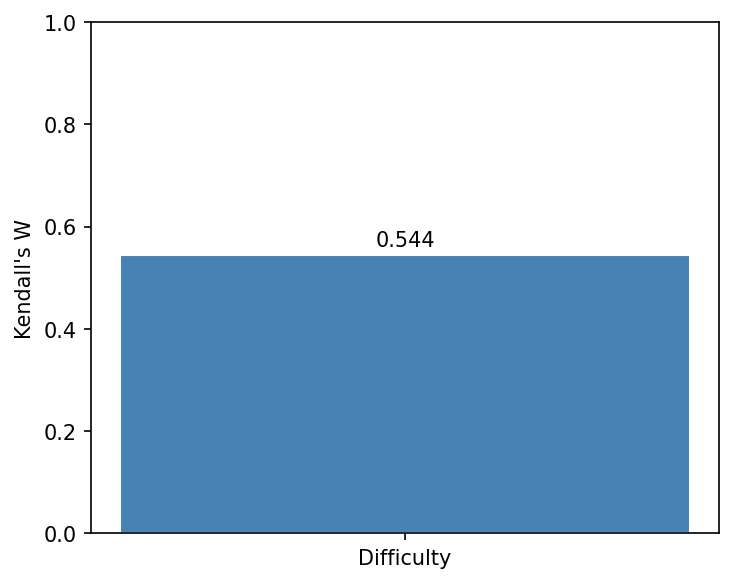
\includegraphics[width=\linewidth]{gsm_1pl_kendalls_w}
    \caption{MGSM 1PL}\label{fig:gsm_1pl_kw}
  \end{subfigure}\hfill
  \begin{subfigure}[t]{0.32\linewidth}
    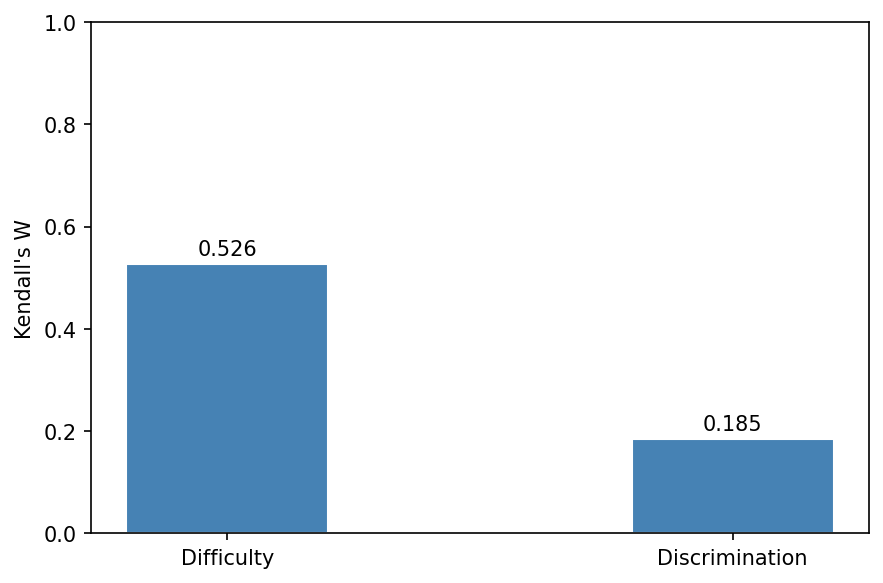
\includegraphics[width=\linewidth]{gsm_2pl_kendalls_w}
    \caption{MGSM 2PL}\label{fig:gsm_2pl_kw}
  \end{subfigure}\hfill
  \begin{subfigure}[t]{0.32\linewidth}
    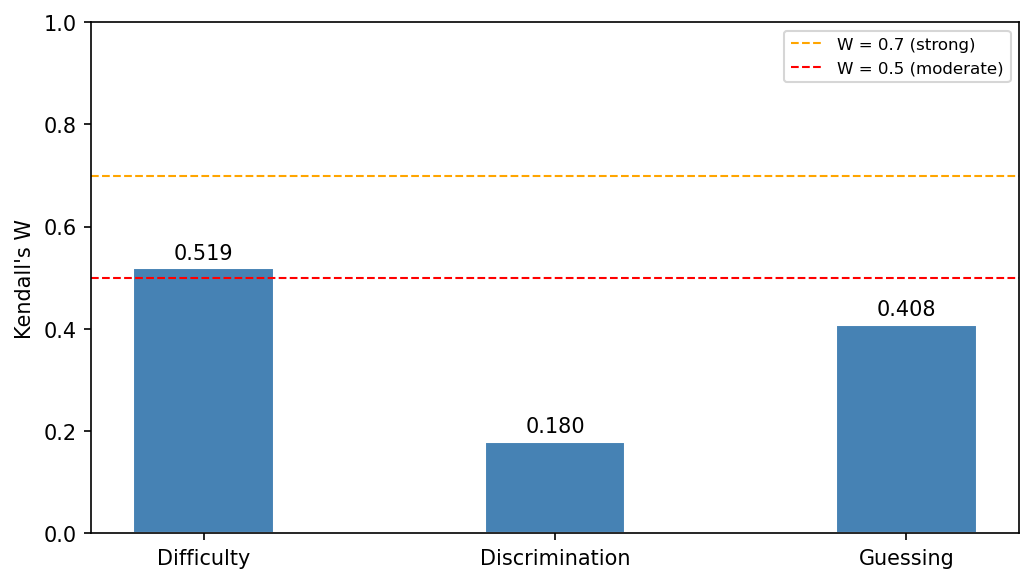
\includegraphics[width=\linewidth]{gsm_3pl_kendalls_w}
    \caption{MGSM 3PL}\label{fig:gsm_3pl_kw}
  \end{subfigure}
  \begin{subfigure}[t]{0.32\linewidth}
    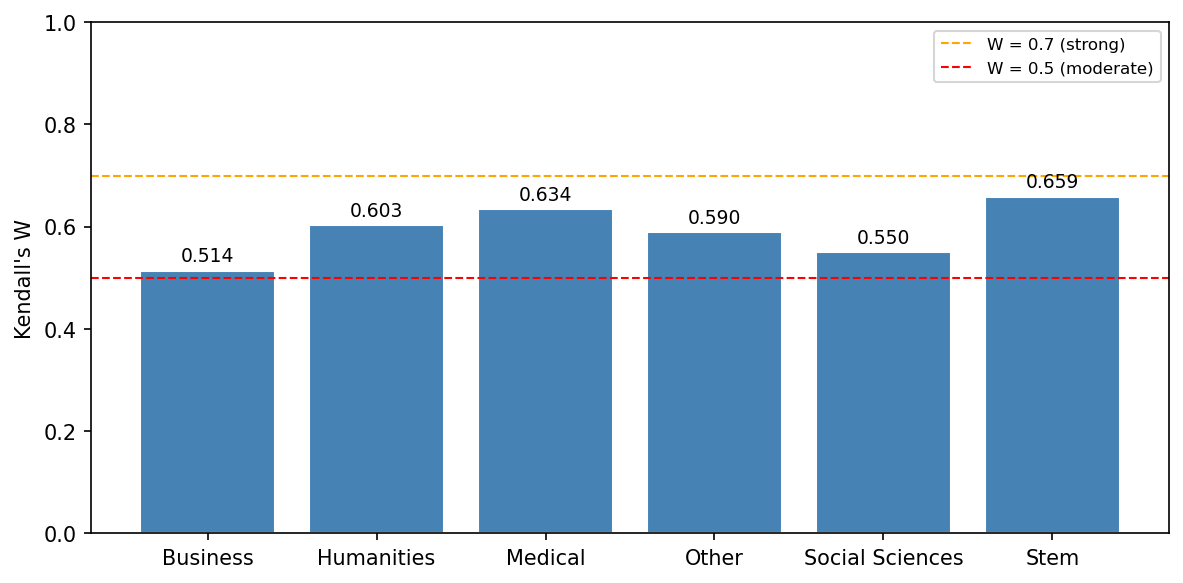
\includegraphics[width=\linewidth]{mmlu_1pl_kendalls_w}
    \caption{MMLU 1PL}\label{fig:mmlu_1pl_kw}
  \end{subfigure}\hfill
  \begin{subfigure}[t]{0.32\linewidth}
    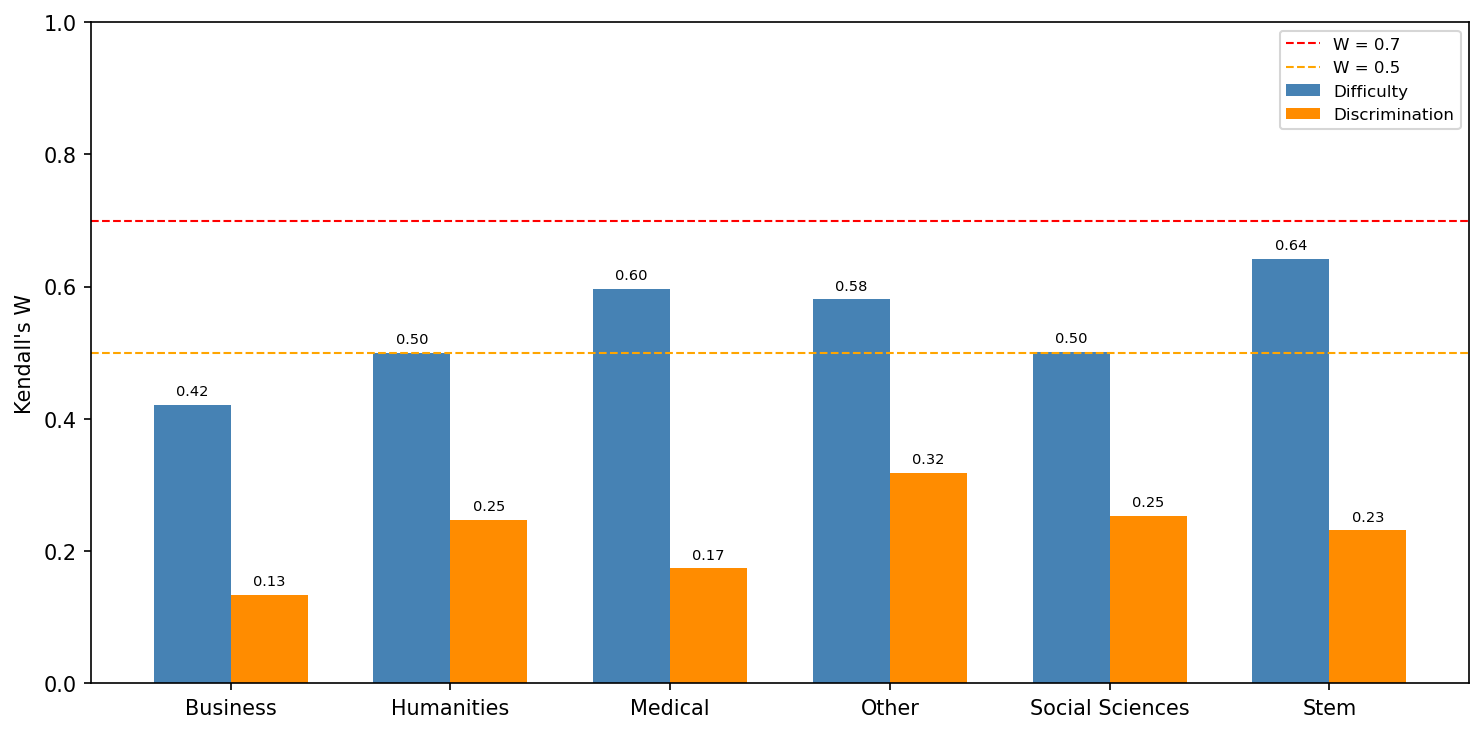
\includegraphics[width=\linewidth]{mmlu_2pl_kendalls_w}
    \caption{MMLU 2PL}\label{fig:mmlu_2pl_kw}
  \end{subfigure}\hfill
  \begin{subfigure}[t]{0.32\linewidth}
    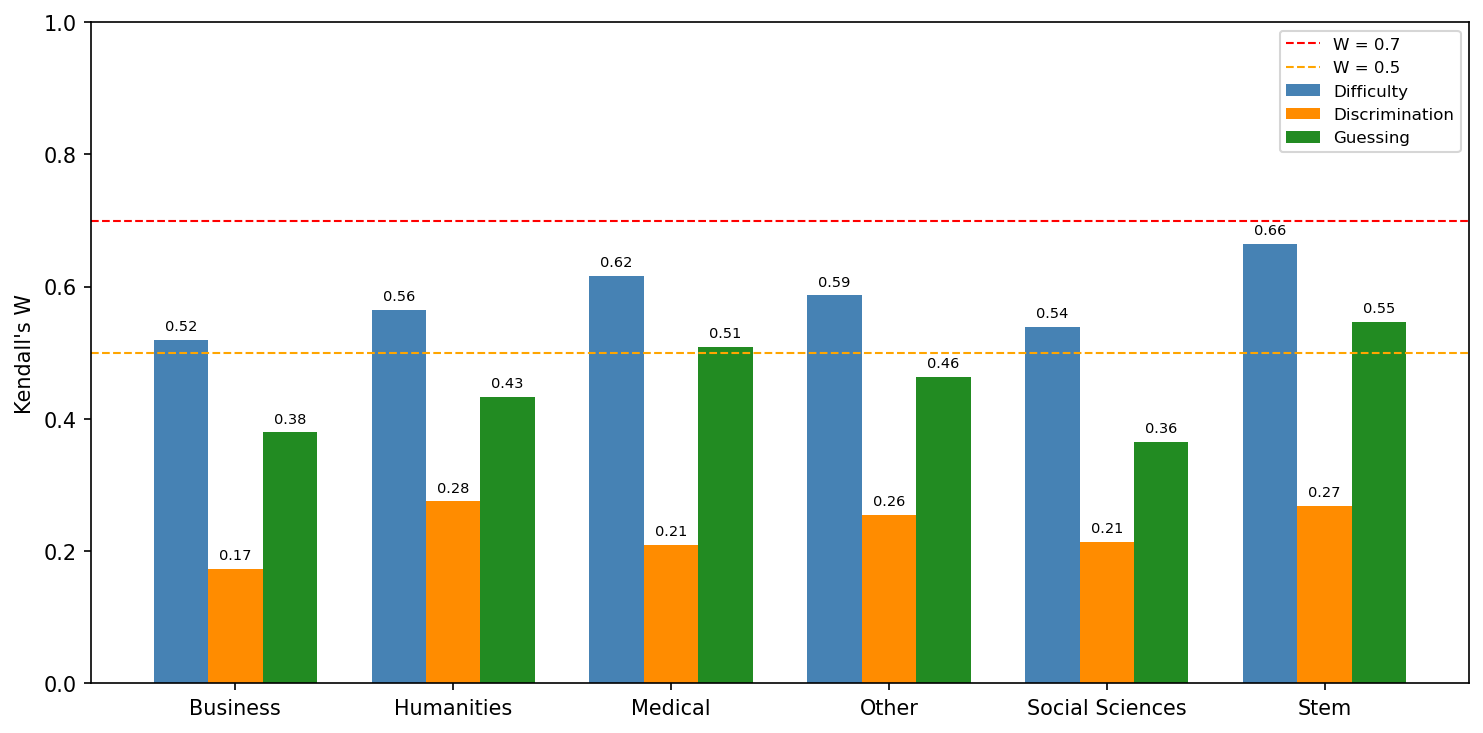
\includegraphics[width=\linewidth]{mmlu_3pl_kendalls_w}
    \caption{MMLU 3PL}\label{fig:mmlu_3pl_kw}
  \end{subfigure}
  \caption{Kendall's $W$ concordance across languages for MGSM (top row) and MMLU
  (bottom row) under 1PL, 2PL, and 3PL models. Dashed lines mark moderate ($W=0.5$)
  and strong ($W=0.7$) concordance thresholds. For MMLU, each bar is one domain;
  for MGSM, each bar is one parameter type.}
  \label{fig:kendalls_w}
\end{figure*}

\begin{itemize}

  \item \textbf{1PL (Rasch model).}
  The response probability is
  $P(X_{ij}=1) = \sigma(\theta_i - b_j)$,
  where $\theta_i$ is the ability of model $i$ and $b_j$ is the difficulty of item $j$. Trained for 2{,}000 epochs with learning rate $\eta = 0.1$.

  \item \textbf{2PL.}
  The response probability is
  $P(X_{ij}=1) = \sigma\!\left(a_j(\theta_i - b_j)\right)$,
  adding a per-item discrimination parameter $a_j > 0$ that scales how sharply the
  item distinguishes between high- and low-ability models.
  Fitted via MAP for 4{,}000 epochs with learning rate $\eta = 0.05$.

  \item \textbf{3PL.}
  The response probability is
  $P(X_{ij}=1) = c_j + (1 - c_j)\,\sigma\!\left(a_j(\theta_i - b_j)\right)$,
  where $c_j \in [0,1]$ is a lower asymptote (pseudo-guessing parameter) that
  models the probability of a correct response by a minimally-capable model, capturing
  chance-level or knowledge-independent success on an item.
  Fitted via MAP for 6{,}000 epochs with learning rate $\eta = 0.05$.

\end{itemize}

\noindent
The 1PL model uses dropout ($p = 0.5$) and vague priors as implemented in \texttt{py-irt}; epoch count was determined empirically by inspecting the per-epoch ELBO loss curve (set to 2{,}000 at the point of visible stabilisation) and parameters at the minimum-ELBO epoch are retained. For 2PL and 3PL, MAP epoch counts (4{,}000 and 6{,}000 respectively) were selected by monitoring the MAP objective; the best parameter state across all epochs and restarts is retained. To ensure that cross-lingual differences in parameter estimates reflect genuine cross-lingual variation rather than poor within-language fit, we verify that all three variants achieve monotonically improving fit across all 53 benchmark slices (3PL $>$ 2PL $>$ 1PL; \autoref{app:withinlangfits})

\subsection{IRT Analysis}

We conduct two sets of experiments to assess whether IRT parameters are consistent across language versions of these benchmarks \footnote{All code and data will be released upon publication.}.

\textbf{Cross-lingual Consistency Analysis} (§\ref{sec:cross_lingual}) examines whether item parameters are stable across languages using four measures:
(i)~Kendall's $W \in [0,1]$, the coefficient of concordance across all $|\mathcal{L}|$ languages simultaneously ($W=1$: identical item rankings; $W\approx 0$: chance);
(ii)~Spearman Correlations $\rho \in [-1,1]$, the monotonic rank correlation between each language pair, displayed as a $|\mathcal{L}|\times|\mathcal{L}|$ heatmap;
(iii)~Per-Item Rank Deviation, the variability of each item's difficulty rank across languages, where high values flag linguistically unstable items;
(iv)~Language Clustering (average linkage on Spearman distance $1-\rho$) grouping languages by similarity of their IRT profiles, and accuracy-based groupings via Mantel Test.

\textbf{Subset Analysis} (§\ref{sec:iif}) evaluates IRT filtering along two dimensions. (i)~ Cross-Model IIF Concordance: items are ranked by their Item Information Function (IIF) at $\theta=0$ under each IRT model variant, and pairwise Jaccard similarity of the top-50\% subsets is measured across benchmark slices to assess whether model choice affects item selection; (ii) Subset Ranking Fidelity: whether accuracy on the IRT-selected subset reproduces model rankings on the full benchmark, evaluated both within-language and cross-lingually, under in-sample and held-out model splits.

\section{Results}
\label{sec:results}

\subsection{Cross-Lingual Consistency Analysis}
\label{sec:cross_lingual}

\paragraph{Kendall's $W$ Concordance}

\begin{table}[t]
  \centering
  \small
  \begin{tabular}{lcccc}
    \toprule
    & \multicolumn{2}{c}{\textbf{Science}} & \multicolumn{2}{c}{\textbf{Non-science}} \\
    \cmidrule(lr){2-3}\cmidrule(lr){4-5}
    \textbf{Model} & $W$ & $\bar{\rho}$ & $W$ & $\bar{\rho}$ \\
    \midrule
    1PL & 0.647 & 0.588 & 0.564 & 0.492 \\
    2PL & 0.620 & 0.559 & 0.501 & 0.420 \\
    3PL & 0.640 & 0.581 & 0.553 & 0.479 \\
    \bottomrule
  \end{tabular}
  \caption{ Kendall's $W$ and Mean Pairwise Spearman $\bar{\rho}$ for item
    \emph{difficulty} across languages, averaged over science (STEM + Medical)
    and non-science (Business + Humanities + Other + Social Sciences) domains
    of MMLU, for each IRT model variant.}
  \label{tab:science_vs_nonsci}
\end{table}

\autoref{fig:kendalls_w} shows that difficulty concordance is maintained across model complexities, while discrimination parameters are substantially less cross-lingually stable. Under 1PL, both benchmarks yield moderate difficulty concordance: MGSM at $W = 0.544$ and MMLU domains ranging from $W \in [0.514, 0.659]$ (all six domains exceeding the moderate-agreement threshold\footnote{We adopt $W=0.5$ and $W=0.7$ as moderate and strong concordance thresholds by analogy with conventional correlation effect-size interpretation; no universally agreed scale exists for Kendall's $W$. Practically, $W=0.5$ implies that the average monotonic agreement in item difficulty ranks substantially exceeds chance. We interpret this as \emph{partial} cross-lingual
generalization rather than strong invariance, and our conclusions are framed
accordingly.}). Under 2PL, difficulty concordance is maintained: MGSM $W_\text{diff} = 0.526$ (barely below 1PL), MMLU $W_\text{diff} \in [0.421, 0.642]$. Under 3PL, difficulty concordance is similarly preserved (MGSM $W_\text{diff} = 0.519$; MMLU $W_\text{diff} \in [0.520, 0.664]$). The discrimination parameter, by contrast, shows substantially lower cross-lingual agreement across both 2PL (MGSM $W_\text{disc} = 0.185$; MMLU $W_\text{disc} \in [0.134, 0.319]$) and 3PL ($W_\text{disc}$ similarly low). The guessing parameter $c$ under 3PL retains moderate concordance on both MGSM ($W = 0.408$) and MMLU ($W \in [0.365, 0.547]$).

A cross-domain analysis (\autoref{tab:science_vs_nonsci}) of item \textit{difficulty} groups MMLU domains into science (STEM + Medical) and non-science (Business + Humanities + Other + Social Sciences), revealing a persistent science advantage that holds across all model variants. %Under 1PL, science domains show higher concordance ($W = 0.647$, $\bar{\rho} = 0.588$) than non-science ($W = 0.564$, $\bar{\rho} = 0.492$). Under 2PL and 3PL, science domains continue to exceed non-science.(2PL: science $W = 0.620$, $\bar{\rho} = 0.559$; non-science $W = 0.501$, $\bar{\rho} = 0.420$; 3PL: science $W = 0.640$, $\bar{\rho} = 0.581$; non-science $W = 0.553$, $\bar{\rho} = 0.479$). 
Scientific domains, where mathematical and factual content is more likely to be language-invariant, yield more consistent IRT parameters across languages.

%In Figure~\ref{fig:kendalls_w}, we report Kendall's $W$ across all three IRT model variants for both benchmarks. For MGSM, 1PL yields moderate difficulty concordance ($W = 0.544$) across 11 languages. Introducing discrimination in 2PL causes a sharp drop ($W_\text{diff} = 0.163$, $W_\text{disc} = 0.125$), and 3PL falls further still ($W_\text{diff} = 0.067$, $W_\text{disc} = 0.079$); the guessing parameter $c$ is a notable exception, retaining moderate concordance ($W = 0.404$). Across all MGSM variants, discrimination is consistently less stable across languages than difficulty. MMLU shows higher absolute concordance but the same downward trend across PL complexity. Under 1PL, all six domains exceed the moderate-agreement threshold ($W \in [0.514, 0.659]$), with STEM domains the most stable and Business the least. Under 2PL, concordance falls but remains higher than MGSM: difficulty ranges from $W = 0.294$ (Social Sciences) to $W = 0.410$ (Medical), and, unlike MGSM, discrimination exceeds difficulty concordance in every domain ($W \in [0.374, 0.538]$). Under 3PL, difficulty and discrimination both drop sharply in most domains, though guessing concordance stays high across all domains ($W \in [0.512, 0.615]$). As seen in Table~\ref{tab:science_vs_nonsci}, domain-level variation is consistent: scientific domains like STEM and Medical show greater cross-lingual stability than Humanities, Business, and Social Sciences.







\begin{figure}[t]
  \centering
  \begin{subfigure}[t]{0.32\linewidth}
    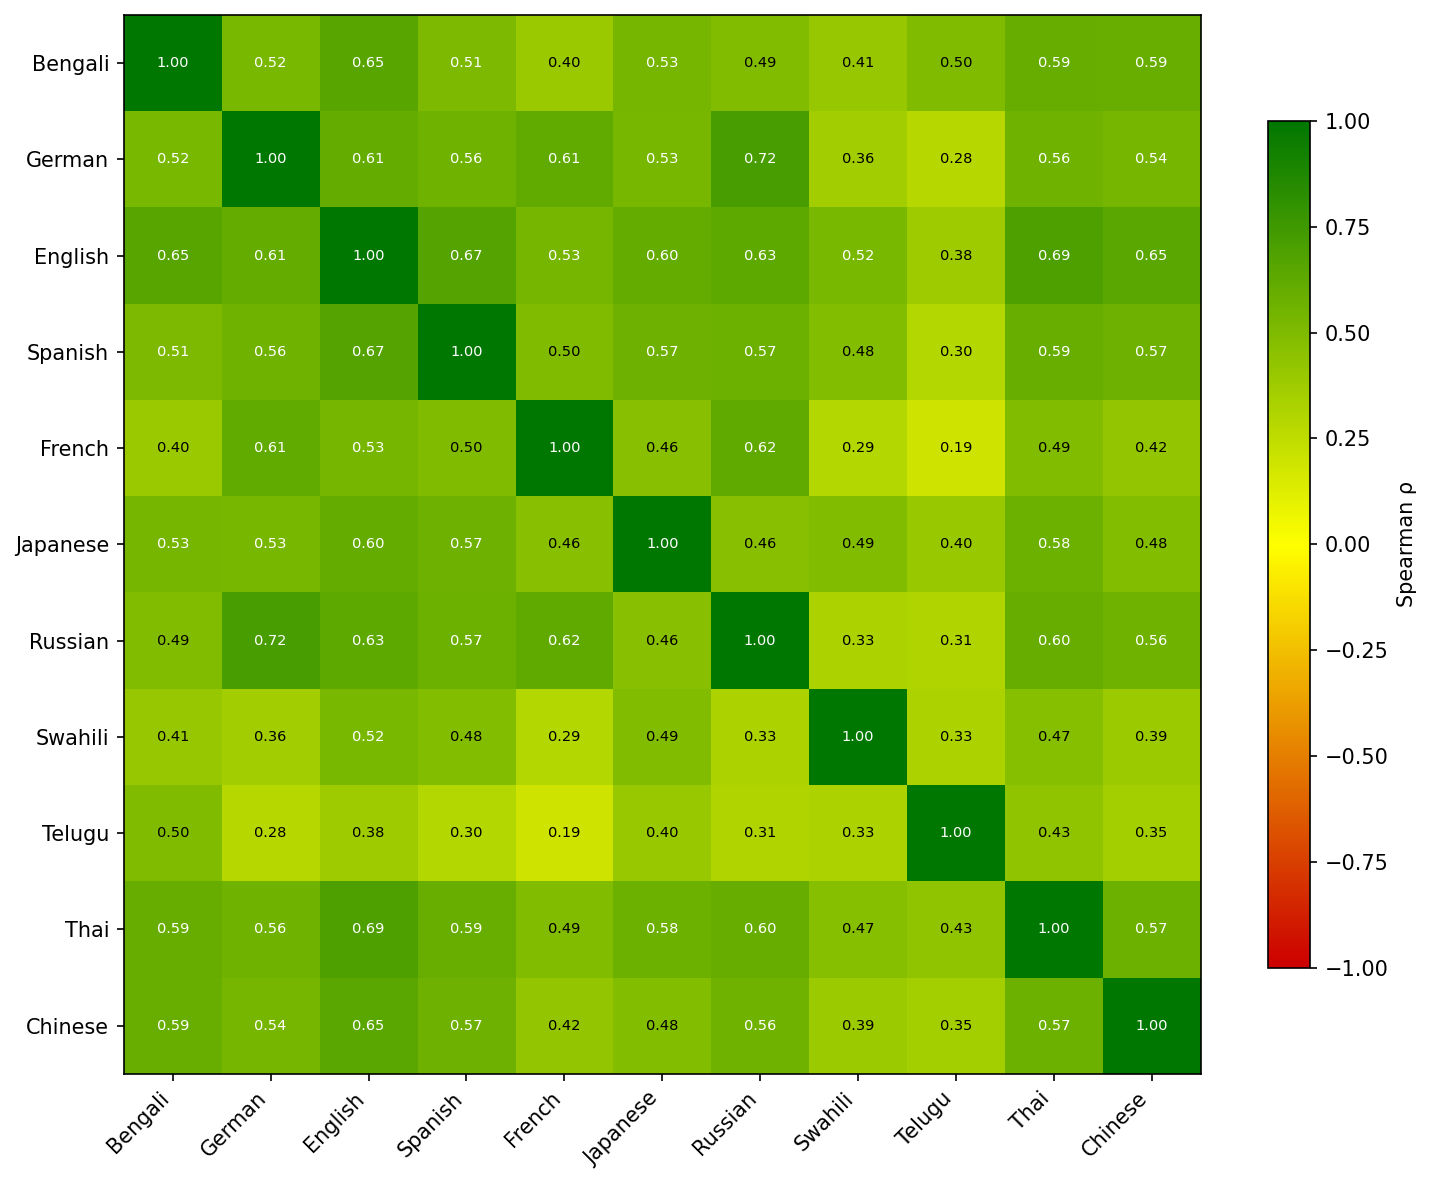
\includegraphics[width=\linewidth]{gsm_1pl_spearman_heatmap}
    \caption{MGSM 1PL}\label{fig:gsm_1pl_sp}
  \end{subfigure}\hfill
  \begin{subfigure}[t]{0.32\linewidth}
    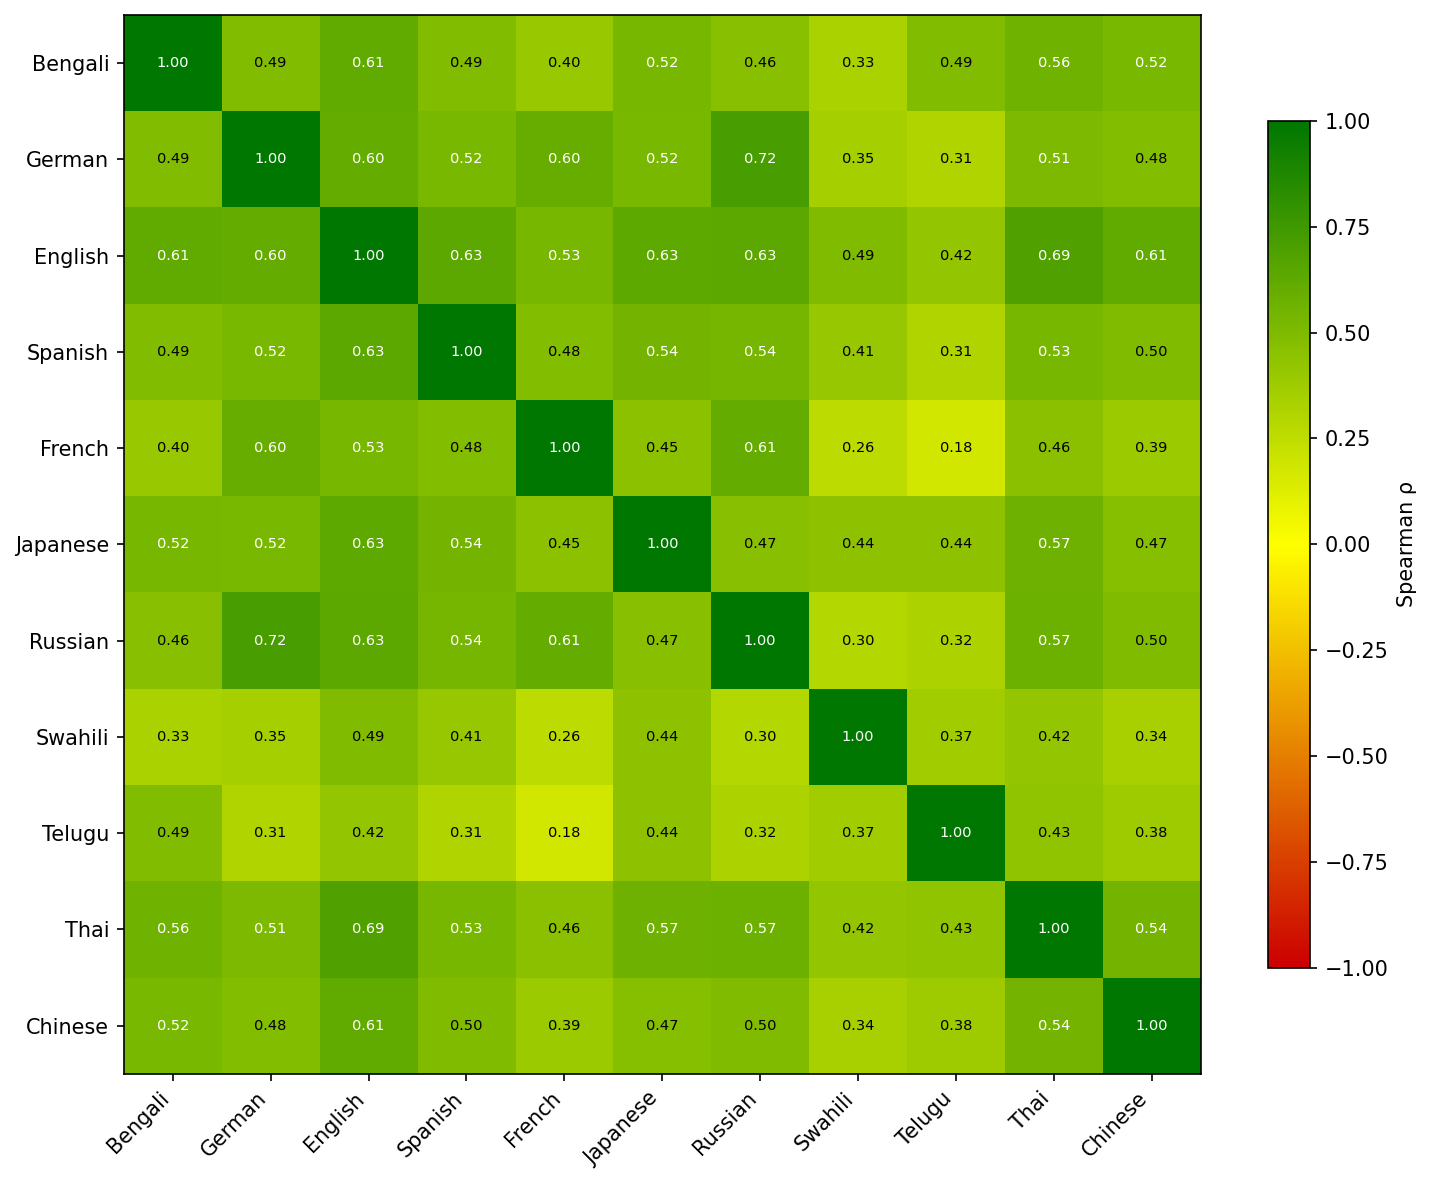
\includegraphics[width=\linewidth]{gsm_2pl_spearman_heatmap_diff}
    \caption{MGSM 2PL}\label{fig:gsm_2pl_sp}
  \end{subfigure}\hfill
  \begin{subfigure}[t]{0.32\linewidth}
    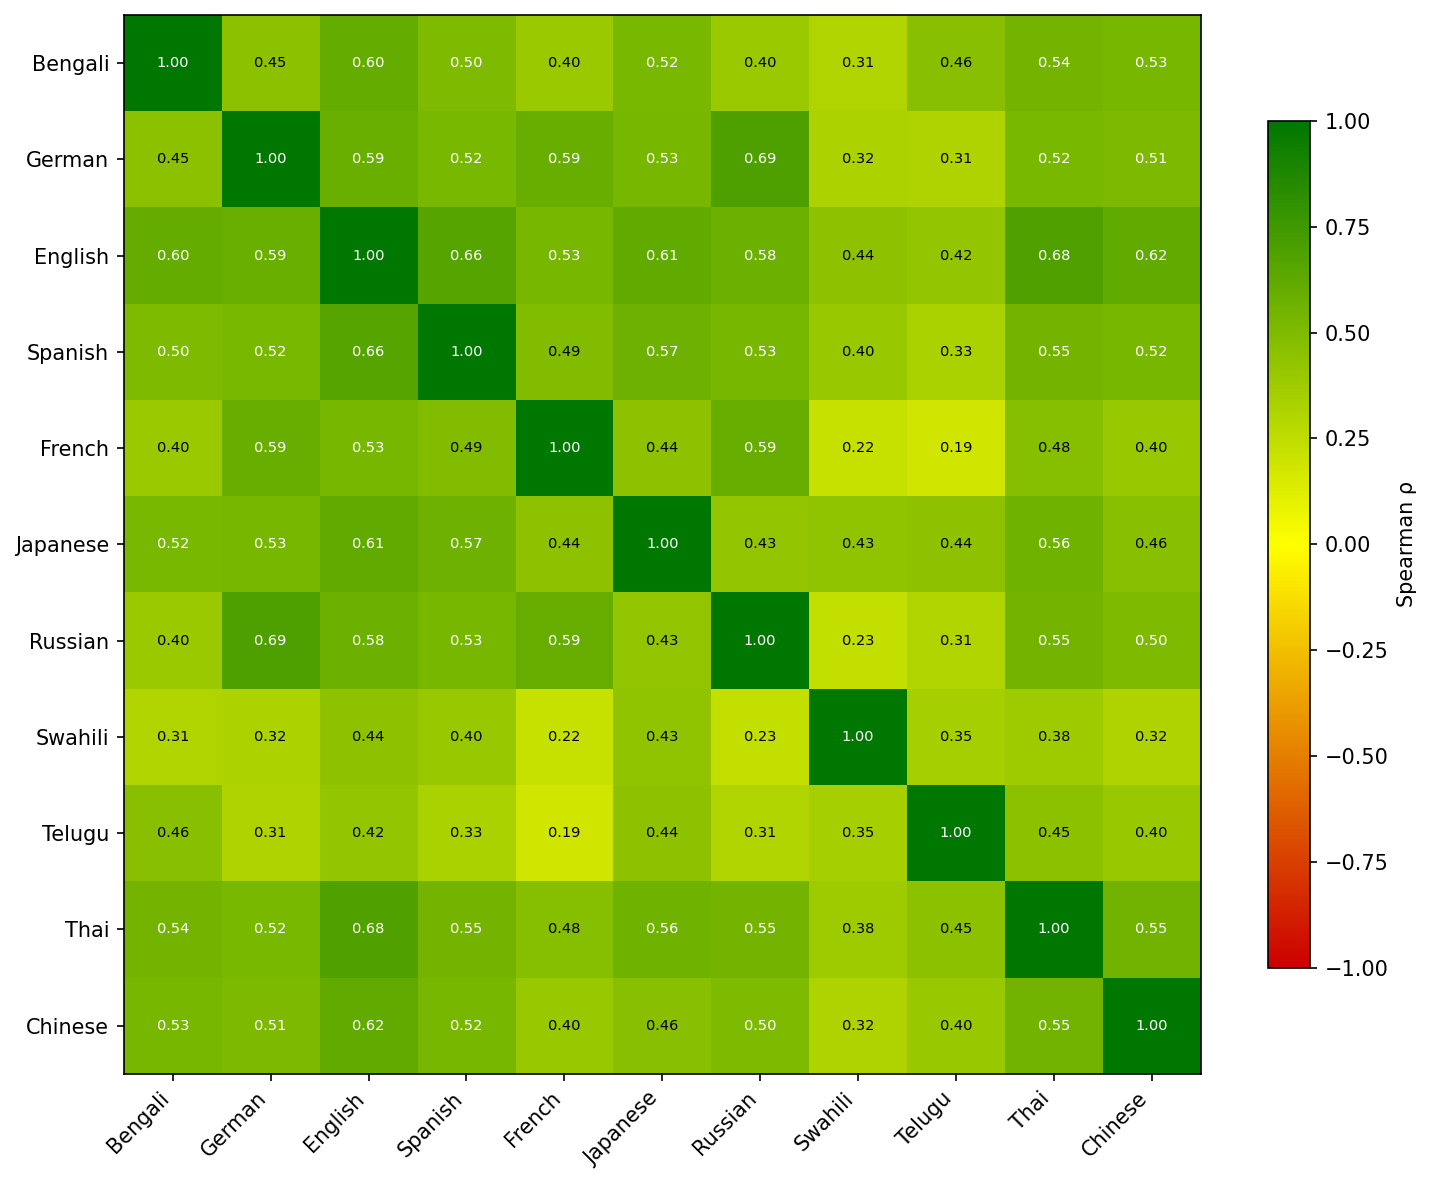
\includegraphics[width=\linewidth]{gsm_3pl_spearman_heatmap_diff}
    \caption{MGSM 3PL}\label{fig:gsm_3pl_sp}
  \end{subfigure}
  \begin{subfigure}[t]{0.32\linewidth}
    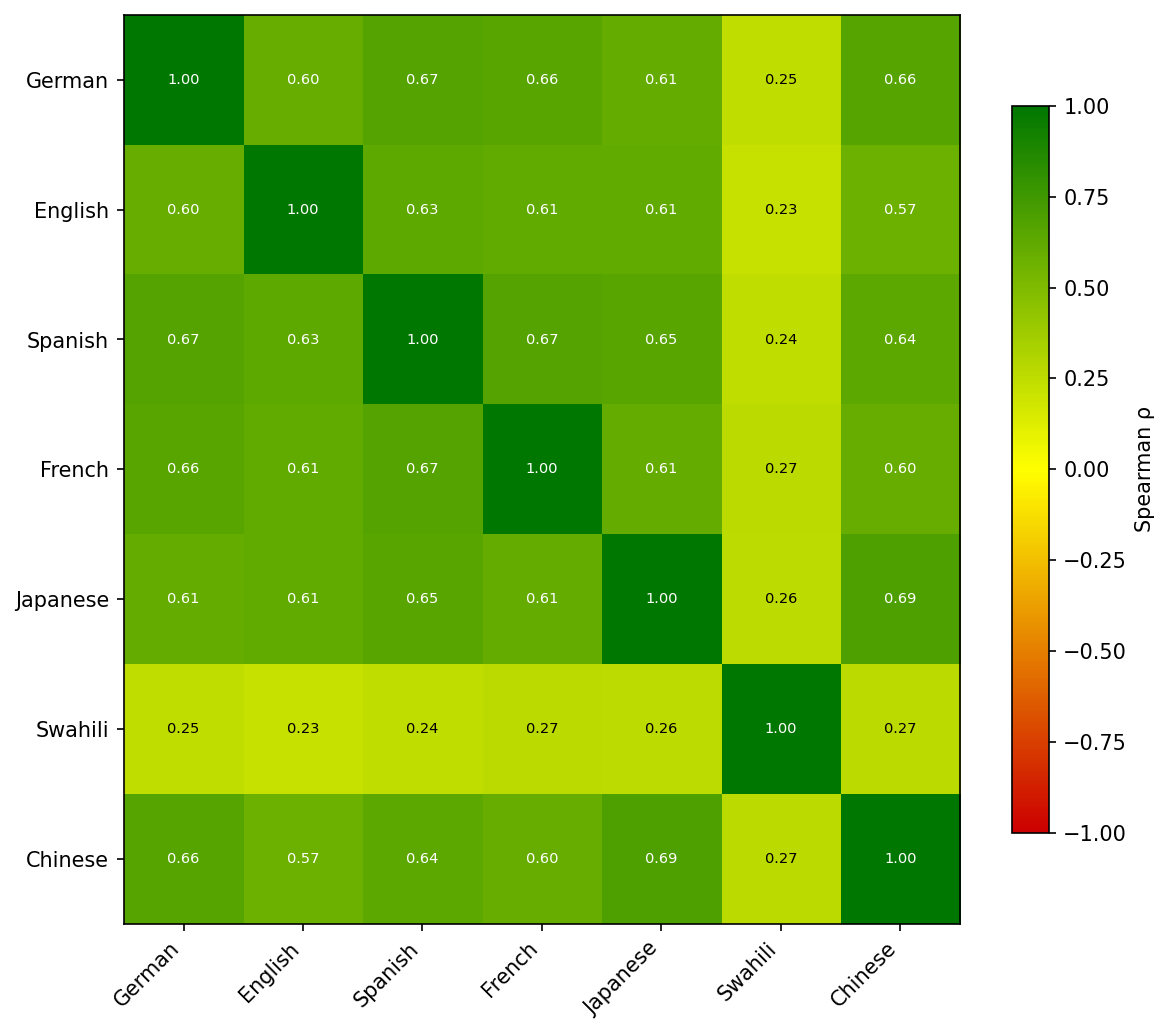
\includegraphics[width=\linewidth]{mmlu_1pl_spearman_heatmap_avg}
    \caption{MMLU 1PL}\label{fig:mmlu_1pl_sp}
  \end{subfigure}\hfill
  \begin{subfigure}[t]{0.32\linewidth}
    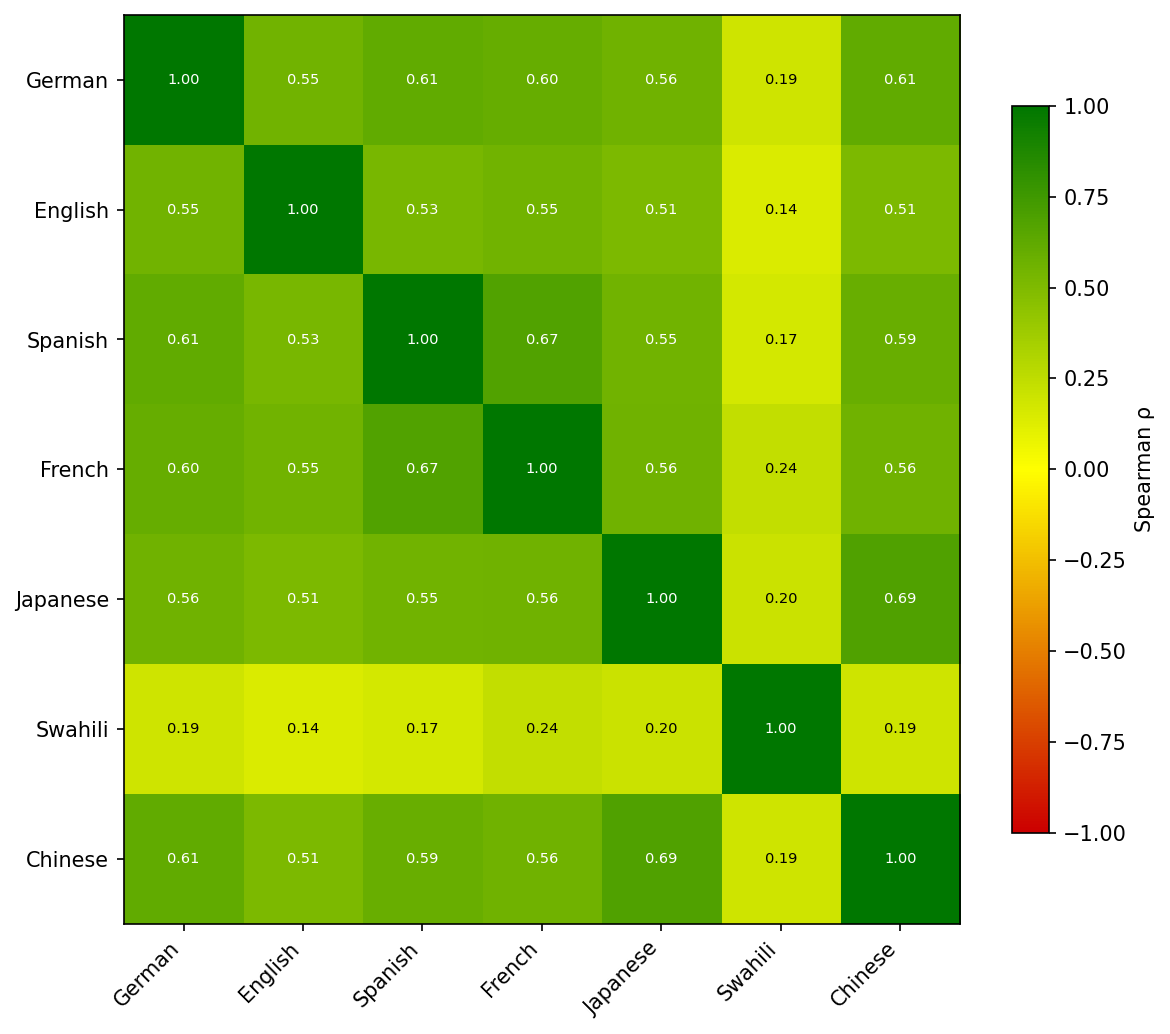
\includegraphics[width=\linewidth]{mmlu_2pl_spearman_heatmap_avg_diff}
    \caption{MMLU 2PL}\label{fig:mmlu_2pl_sp}
  \end{subfigure}\hfill
  \begin{subfigure}[t]{0.32\linewidth}
    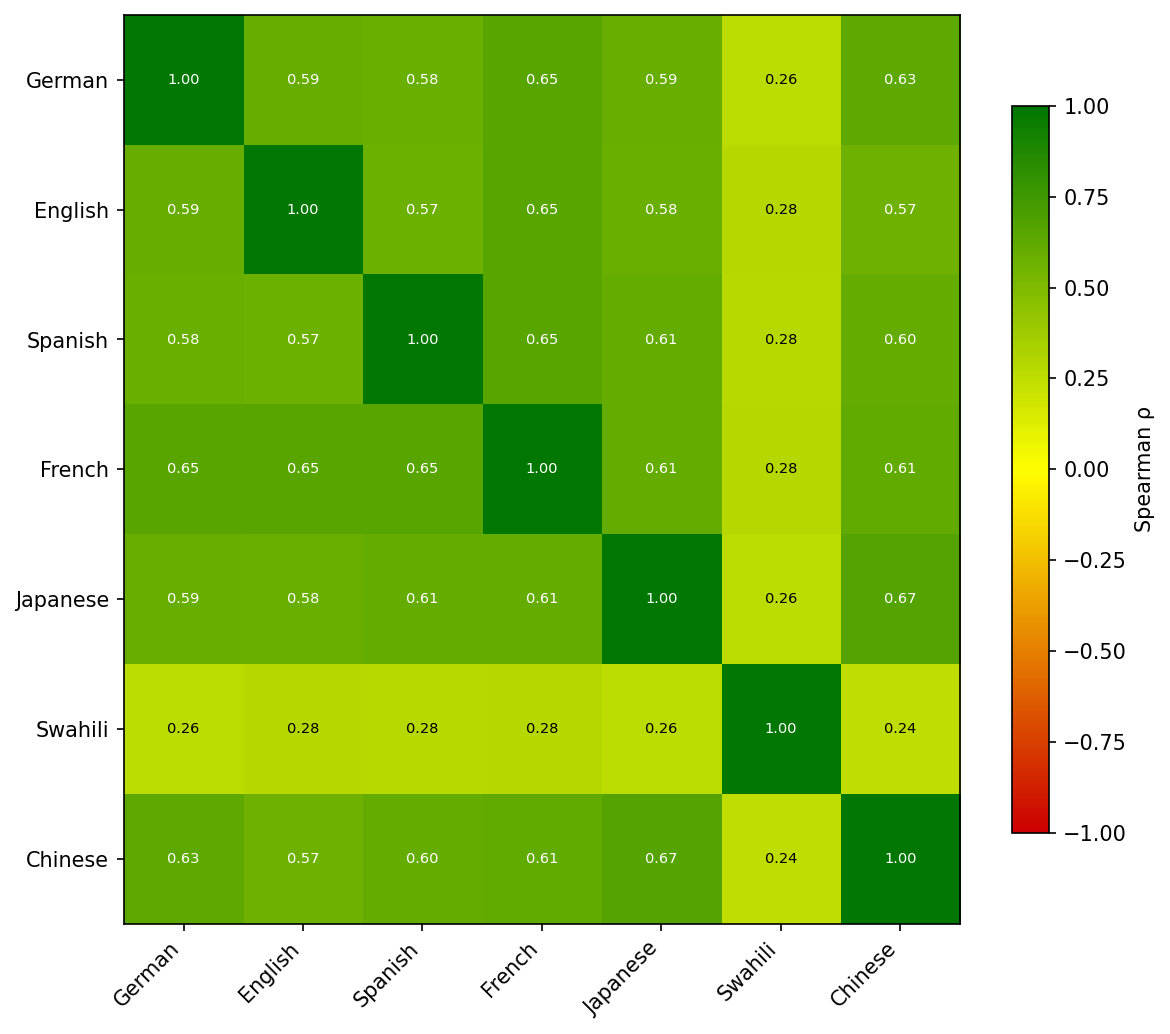
\includegraphics[width=\linewidth]{mmlu_3pl_spearman_heatmap_avg_diff}
    \caption{MMLU 3PL}\label{fig:mmlu_3pl_sp}
  \end{subfigure}
  \caption{Pairwise Spearman rank correlation of item \emph{difficulty} across
    languages for 1PL, 2PL, and 3PL IRT models on MGSM (top row) and MMLU
    (bottom row; each cell is the element-wise average over six domains).
    Colour encodes $\rho \in [-1, +1]$: red $= -1$, yellow $= 0$, green $= +1$.}
  \label{fig:spearman_heatmaps}
\end{figure}

\begin{figure}[t]
  \centering
  % ---- Row 1: MGSM ----
  \begin{subfigure}[t]{0.32\linewidth}
    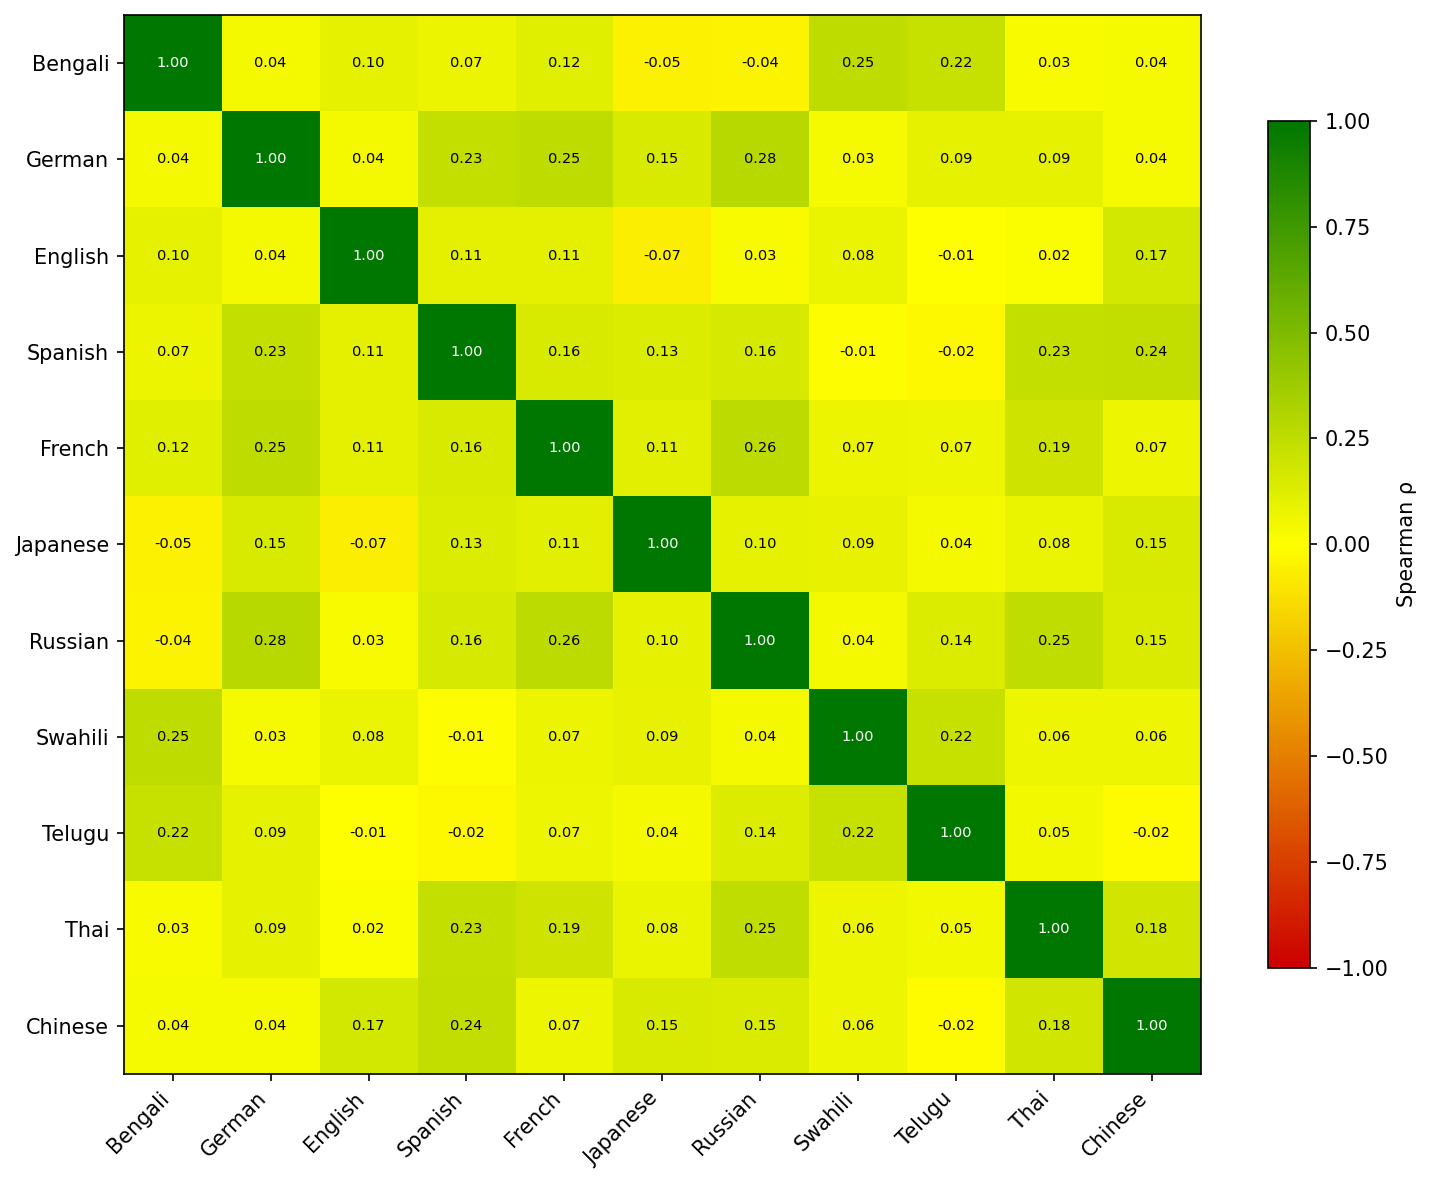
\includegraphics[width=\linewidth]{gsm_2pl_spearman_heatmap_disc}
    \caption{MGSM 2PL}\label{fig:gsm_2pl_disc}
  \end{subfigure}\hfill
  \begin{subfigure}[t]{0.32\linewidth}
    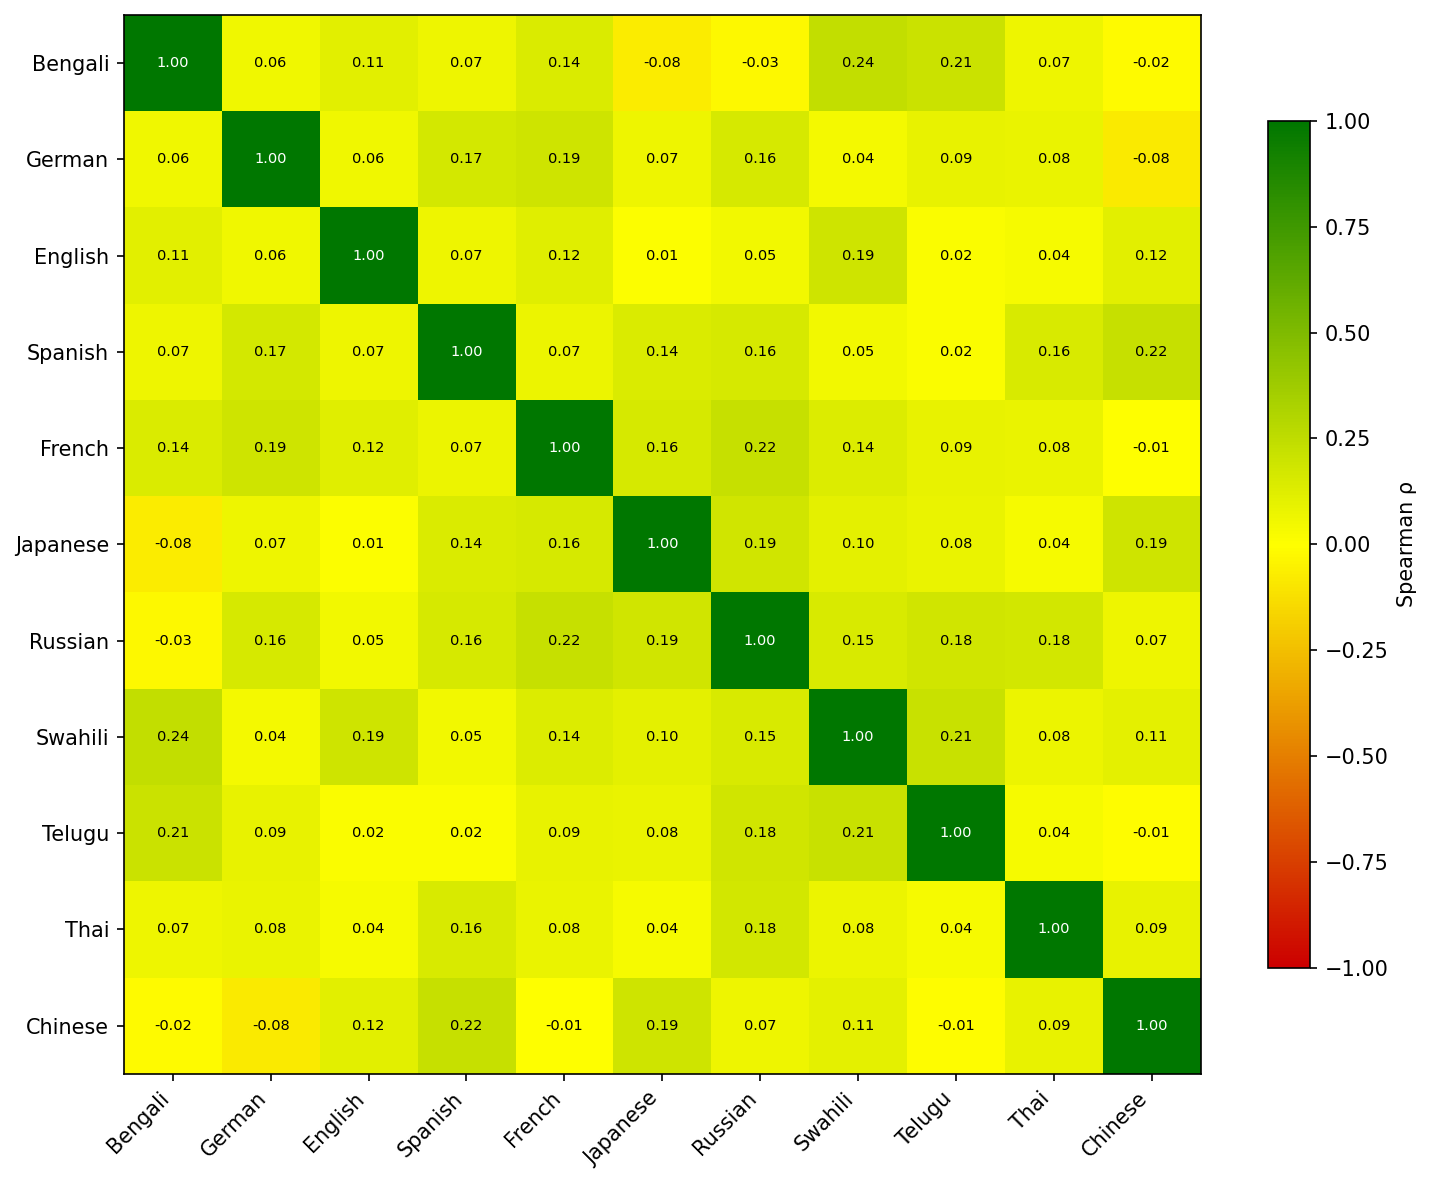
\includegraphics[width=\linewidth]{gsm_3pl_spearman_heatmap_disc}
    \caption{MGSM 3PL}\label{fig:gsm_3pl_disc}
  \end{subfigure}\hfill
  \begin{subfigure}[t]{0.32\linewidth}
    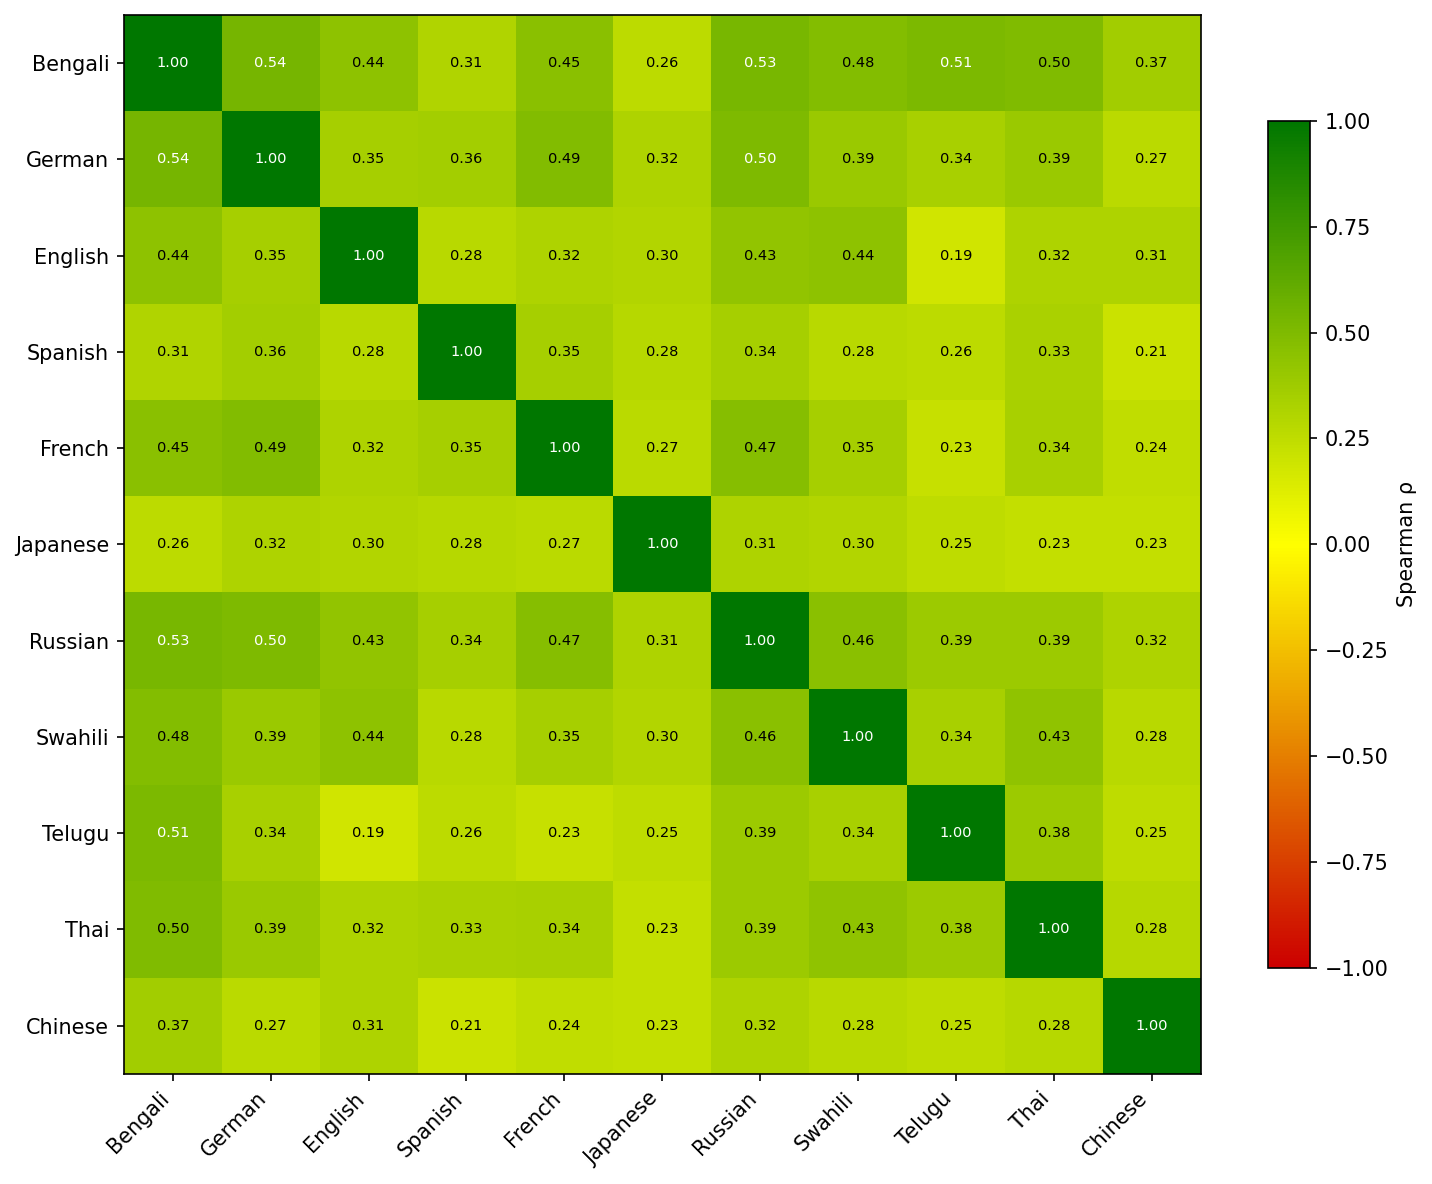
\includegraphics[width=\linewidth]{gsm_3pl_spearman_heatmap_guess}
    \caption{MGSM 3PL}\label{fig:gsm_3pl_guess}
  \end{subfigure}
  % ---- Row 2: MMLU (averaged across domains) ----
  \begin{subfigure}[t]{0.32\linewidth}
    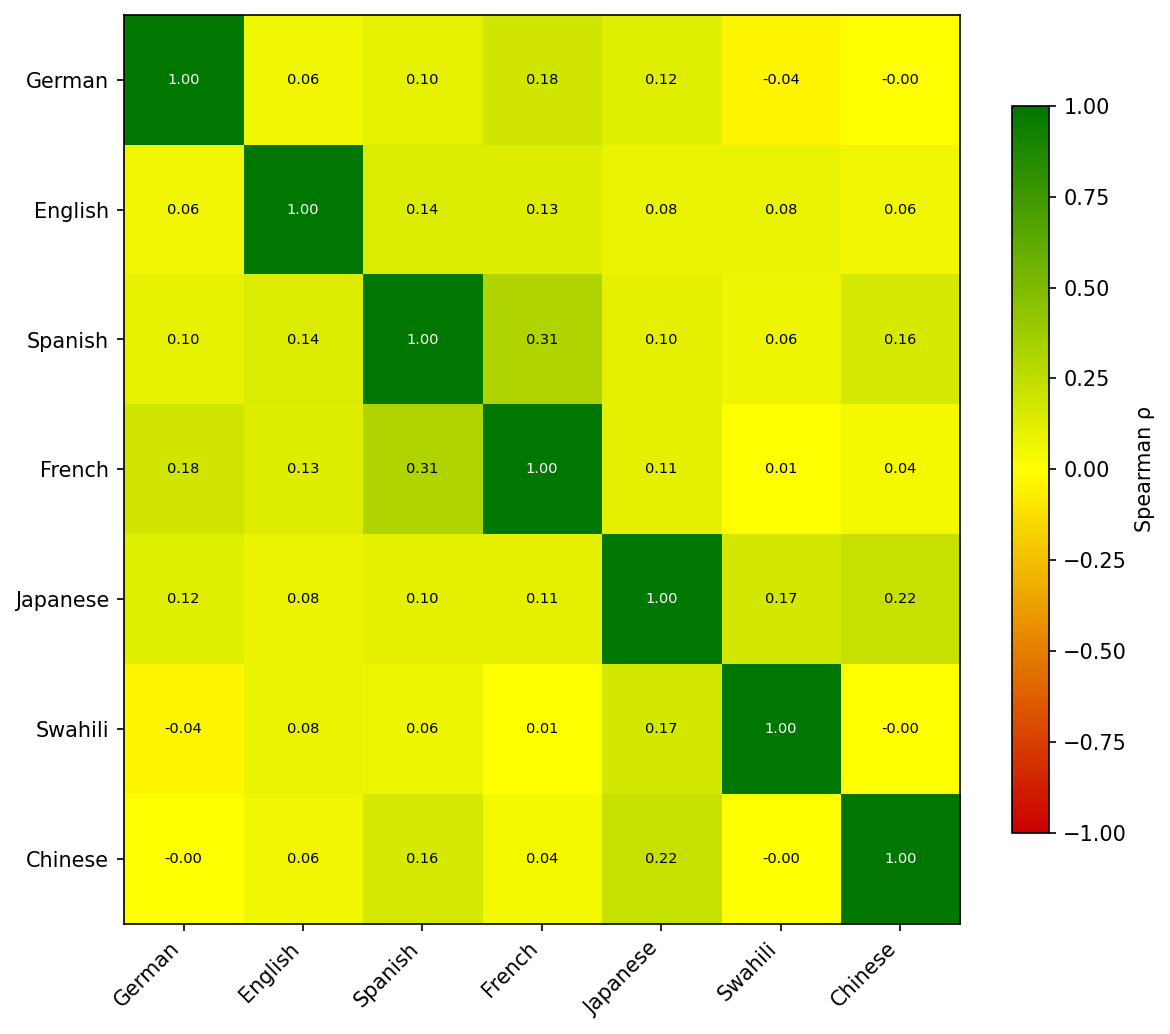
\includegraphics[width=\linewidth]{mmlu_2pl_spearman_heatmap_avg_disc}
    \caption{MMLU 2PL }\label{fig:mmlu_2pl_disc}
  \end{subfigure}\hfill
  \begin{subfigure}[t]{0.32\linewidth}
    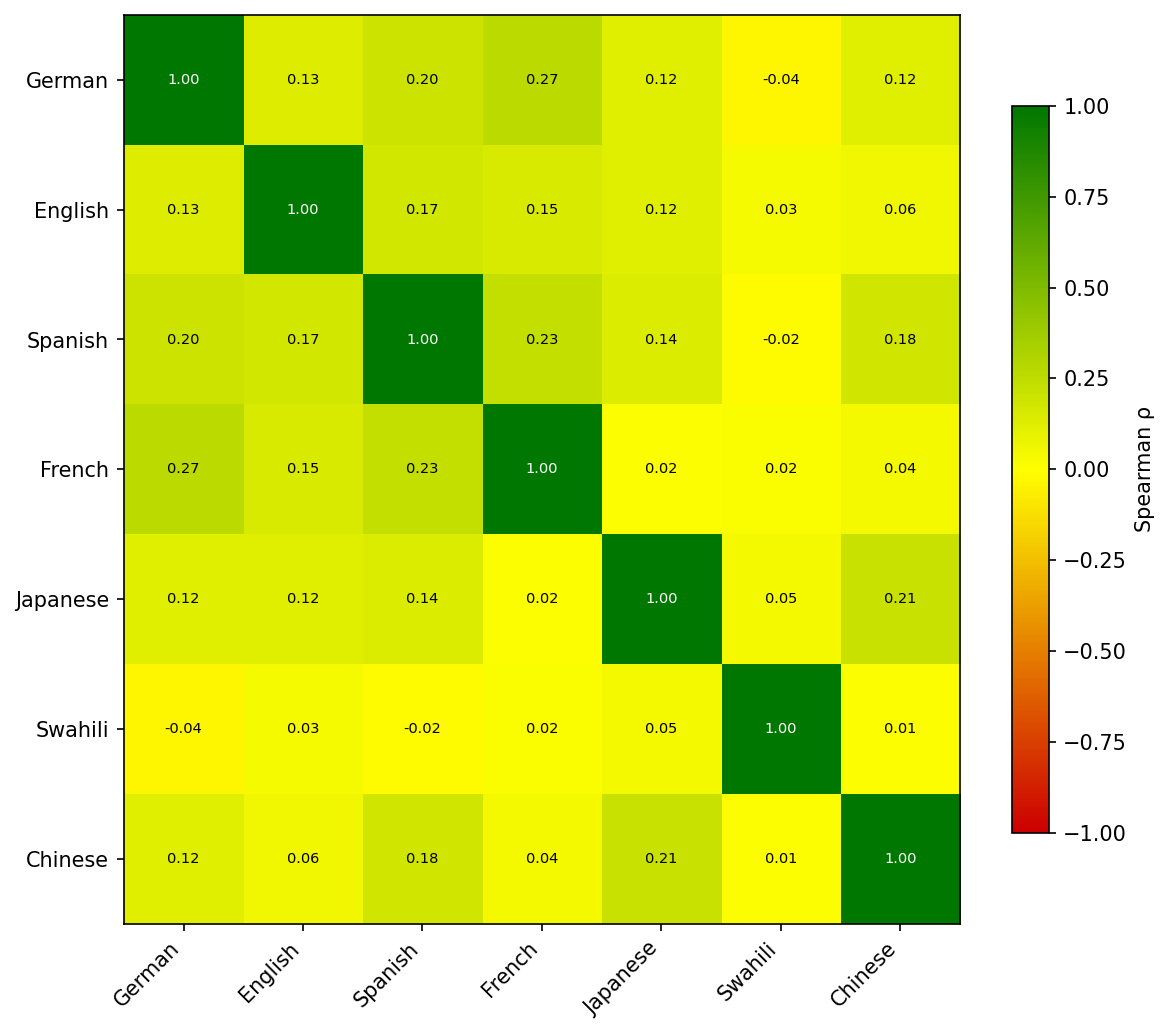
\includegraphics[width=\linewidth]{mmlu_3pl_spearman_heatmap_avg_disc}
    \caption{MMLU 3PL }\label{fig:mmlu_3pl_disc}
  \end{subfigure}\hfill
  \begin{subfigure}[t]{0.32\linewidth}
    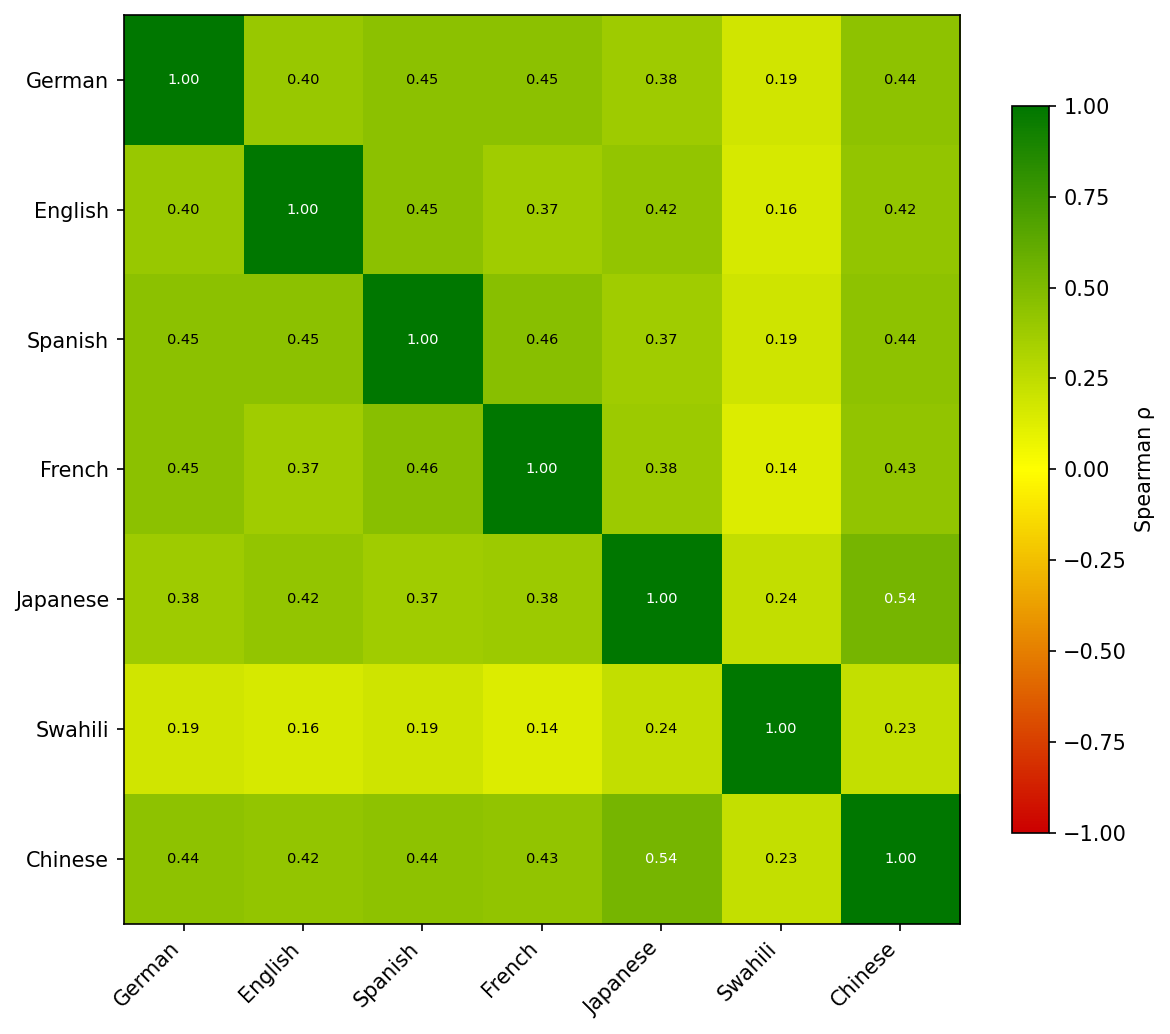
\includegraphics[width=\linewidth]{mmlu_3pl_spearman_heatmap_avg_guess}
    \caption{MMLU 3PL}\label{fig:mmlu_3pl_guess}
  \end{subfigure}
  \caption{Pairwise Spearman rank correlation of item \emph{discrimination} ($a$,
    columns 1--2) and \emph{guessing} ($c$, column 3) across
    languages for MGSM (top row) and MMLU (bottom row; element-wise average
    over six domains). Colour encodes $\rho \in [-1,+1]$: red $= -1$, yellow
    $= 0$, green $= +1$. }
  \label{fig:spearman_disc_lambda}
\end{figure}

\paragraph{Pairwise Spearman Correlations}

\autoref{fig:spearman_heatmaps} shows pairwise item \textit{difficulty} and \autoref{fig:spearman_disc_lambda} shows pairwise item \textit{discrimination} and \textit{guessing }rank correlations across languages for each IRT variant. Under 1PL, all language pairs show positive monotonic agreement on both MGSM (mean $\rho = 0.498$) and MMLU (mean $\rho = 0.524$), with stronger correlations among typologically proximate pairs (e.g.\ German--Russian: $\rho = 0.718$; English--Spanish: $\rho = 0.670$; Japanese--Chinese: $\rho = 0.69$) and weaker but still positive correlations for structurally distant pairs (e.g.\ French--Telugu: $\rho = 0.190$; French--Swahili: $\rho = 0.290$). On MMLU, European languages form a tight cluster ($\rho \in [0.60, 0.67]$), while Swahili is a consistent outlier across both benchmarks. Under 2PL, difficulty correlations show a modest reduction on MGSM (mean $\rho = 0.479$) and MMLU (mean $\rho = 0.466$), with positive values across most language pairs, indicating that 2PL preserves the shared difficulty structure rather than absorbing it into language-specific variance %\footnote{We conduct a discrimination stability analysis for MMLU in \autoref{app:domain_size}).}. 
Under 3PL, difficulty correlations remain similarly positive (MGSM mean $\rho = 0.470$; MMLU mean $\rho = 0.513$). The discrimination parameter $a$ is less cross-lingually stable across both 2PL and 3PL as seen in \autoref{fig:spearman_disc_lambda} (detailed discussion in \autoref{app:heatmaps}), indicating it captures language-idiosyncratic signal. The guessing parameter $c$ under 3PL again shows stronger positive correlations across language pairs ($W = 0.408$ on MGSM; avg $W = 0.456$ on MMLU), with the same Swahili isolation pattern persisting, suggesting that chance-level correctness is among the most translation-stable properties of an item. The cross-domain analysis (\autoref{tab:science_vs_nonsci}) shows that scientific domains in MMLU consistently show higher correlation across languages than non-science domains.

%For the MGSM, under 1PL, we show in Figure~\ref{fig:spearman_heatmaps} the $|\mathcal{L}|\times|\mathcal{L}|$ matrix of item \emph{difficulty} parameter for each IRT model variant. All language pairs show positive monotonic agreement in item difficulty rankings (mean $\rho = 0.498$, range $0.190$--$0.718$), with stronger correlations among typologically proximate pairs (e.g.\ German--Russian: $\rho = 0.718$; English--Spanish: $\rho = 0.670$) and weaker but still positive correlations for structurally distant pairs (e.g.\ French--Telugu: $\rho = 0.190$; French--Swahili: $\rho = 0.290$). The 2PL and 3PL (in Figure \autoref{fig:spearman_disc_lambda} in Appendix~\ref{app:heatmaps}), the difficulty heatmap shifts to near-zero with a mix of positive and negative correlations (mean $\rho = 0.08$ and $-0.027$ respectively), indicating that the additional parameters absorb language-specific variance rather than preserving a shared item structure. The 3PL guessing parameter $c$ is a notable exception: all off-diagonal pairs remain uniformly positive ($W = 0.404$), suggesting it captures a language-invariant property of items i.e.,chance of guessing answers correctly is stable across languages.For MMLU, we observe similar trends. Under 1PL, the domain-averaged heatmap shows uniformly positive correlations across all language pairs (mean $\rho = 0.524$; Figure~\ref{fig:mmlu_1pl_sp}), somewhat stronger than MGSM. European languages form a tight cluster ($\rho \in [0.60, 0.67]$), Japanese--Chinese pair notably strongly ($\rho = 0.69$), and Swahili is the clear outlier with consistently weak correlations against all other languages ($\rho \in [0.23, 0.27]$). Under 2PL and 3PL, difficulty correlations fade to near-zero with a mix of small positive and negative values ( Figure~\ref{fig:mmlu_3pl_sp}), indicating that richer parameterisations overfit to within-language idiosyncrasies. The 3PL guessing parameter again proves exceptional: it preserves strong positive monotonicity across all pairs (avg $W = 0.554$, mean $\rho$ structure closely mirroring 1PL), with Swahili remaining the most isolated language even here (Figure~\ref{fig:mmlu_3pl_guess}). A cross-domain analysis (Table~\ref{tab:science_vs_nonsci}) groups MMLU domains into science (STEM + Medical) and non-science (Business + Humanities + Other + Social Sciences), revealing a persistent stability gap that widens with model complexity . Science retains a residual cross-lingual signal while non-science are consistently lower, suggesting that science items test reasoning steps whose difficulty is partly language-invariant. Detailed domain-wise heatmaps in Figure~\ref{fig:science_vs_nonscience} of Appendix~\ref{app:heatmaps}.



\paragraph{Per-Item Rank Standard Deviation}

\begin{table}[t]
  \centering
  \small
  \begin{tabular}{llcc}
    \toprule
    \textbf{Model} & \textbf{Param} & \textbf{MGSM} & \textbf{MMLU} \\
                   &                & mean [min, max] & mean [min, max] \\
    \midrule
    1PL & diff & 48.5\ \ [2.8,\ \ 91.8] & 14.5\ \ [1.6,\ \ 34.3] \\
    \midrule
    2PL & diff & 49.5\ \ [4.2,\ \ 98.1] & 15.5\ \ [1.8,\ \ 40.0] \\
        & disc & 67.1\ \ [29.4,\ \ 95.6] & 19.4\ \ [2.6,\ \ 47.1] \\
    \midrule
    3PL & diff & 49.9\ \ [5.9,\ \ 99.4] & 14.7\ \ [1.4,\ \ 37.6] \\
        & disc & 67.1\ \ [19.1,\ \ 99.3] & 19.6\ \ [2.0,\ \ 52.1] \\
        & $c$  & 56.3\ \ [6.0,\ \ 85.9] & 17.0\ \ [1.5,\ \ 47.0] \\
    \bottomrule
  \end{tabular}
  \caption{Per-item rank standard deviation across languages for each IRT
    model variant and parameter. MMLU values are pooled across all six domains
    ($n \leq 102$ items per domain). Lower values indicate higher cross-lingual stability.}
  \label{tab:rank_std}
\end{table}

While Kendall's $W$ and Spearman $\rho$ capture aggregate ordering agreement, they mask item-level heterogeneity: per-item rank SD reveals which individual items preserve their difficulty rank across language versions of a benchmark, directly informing which items are most stable across languages in a multilingual compressed benchmark. For MGSM, stability is highly heterogeneous under 1PL, with some items near-fixed across languages and others shifting almost the full rank range (\autoref{tab:rank_std}). Under 2PL and 3PL, difficulty rank SD is essentially unchanged from 1PL (MGSM: 49.5 and 49.9 vs.\ 48.5; MMLU: 15.5 and 14.7 vs.\ 14.5), while discrimination rank SD is substantially higher ($\approx$67 on MGSM). The guessing parameter $c$ shows intermediate rank stability (MGSM: 56.3). For MMLU, the pattern mirrors MGSM: wide spread under 1PL, with difficulty stability maintained or improved under 2PL/3PL, and discrimination consistently less stable (\autoref{fig:gsm_item_rank_stability} and \autoref{fig:mmlu_item_rank_stability} in \autoref{app:rank_stability}).

\begin{figure}[t]
  \centering
  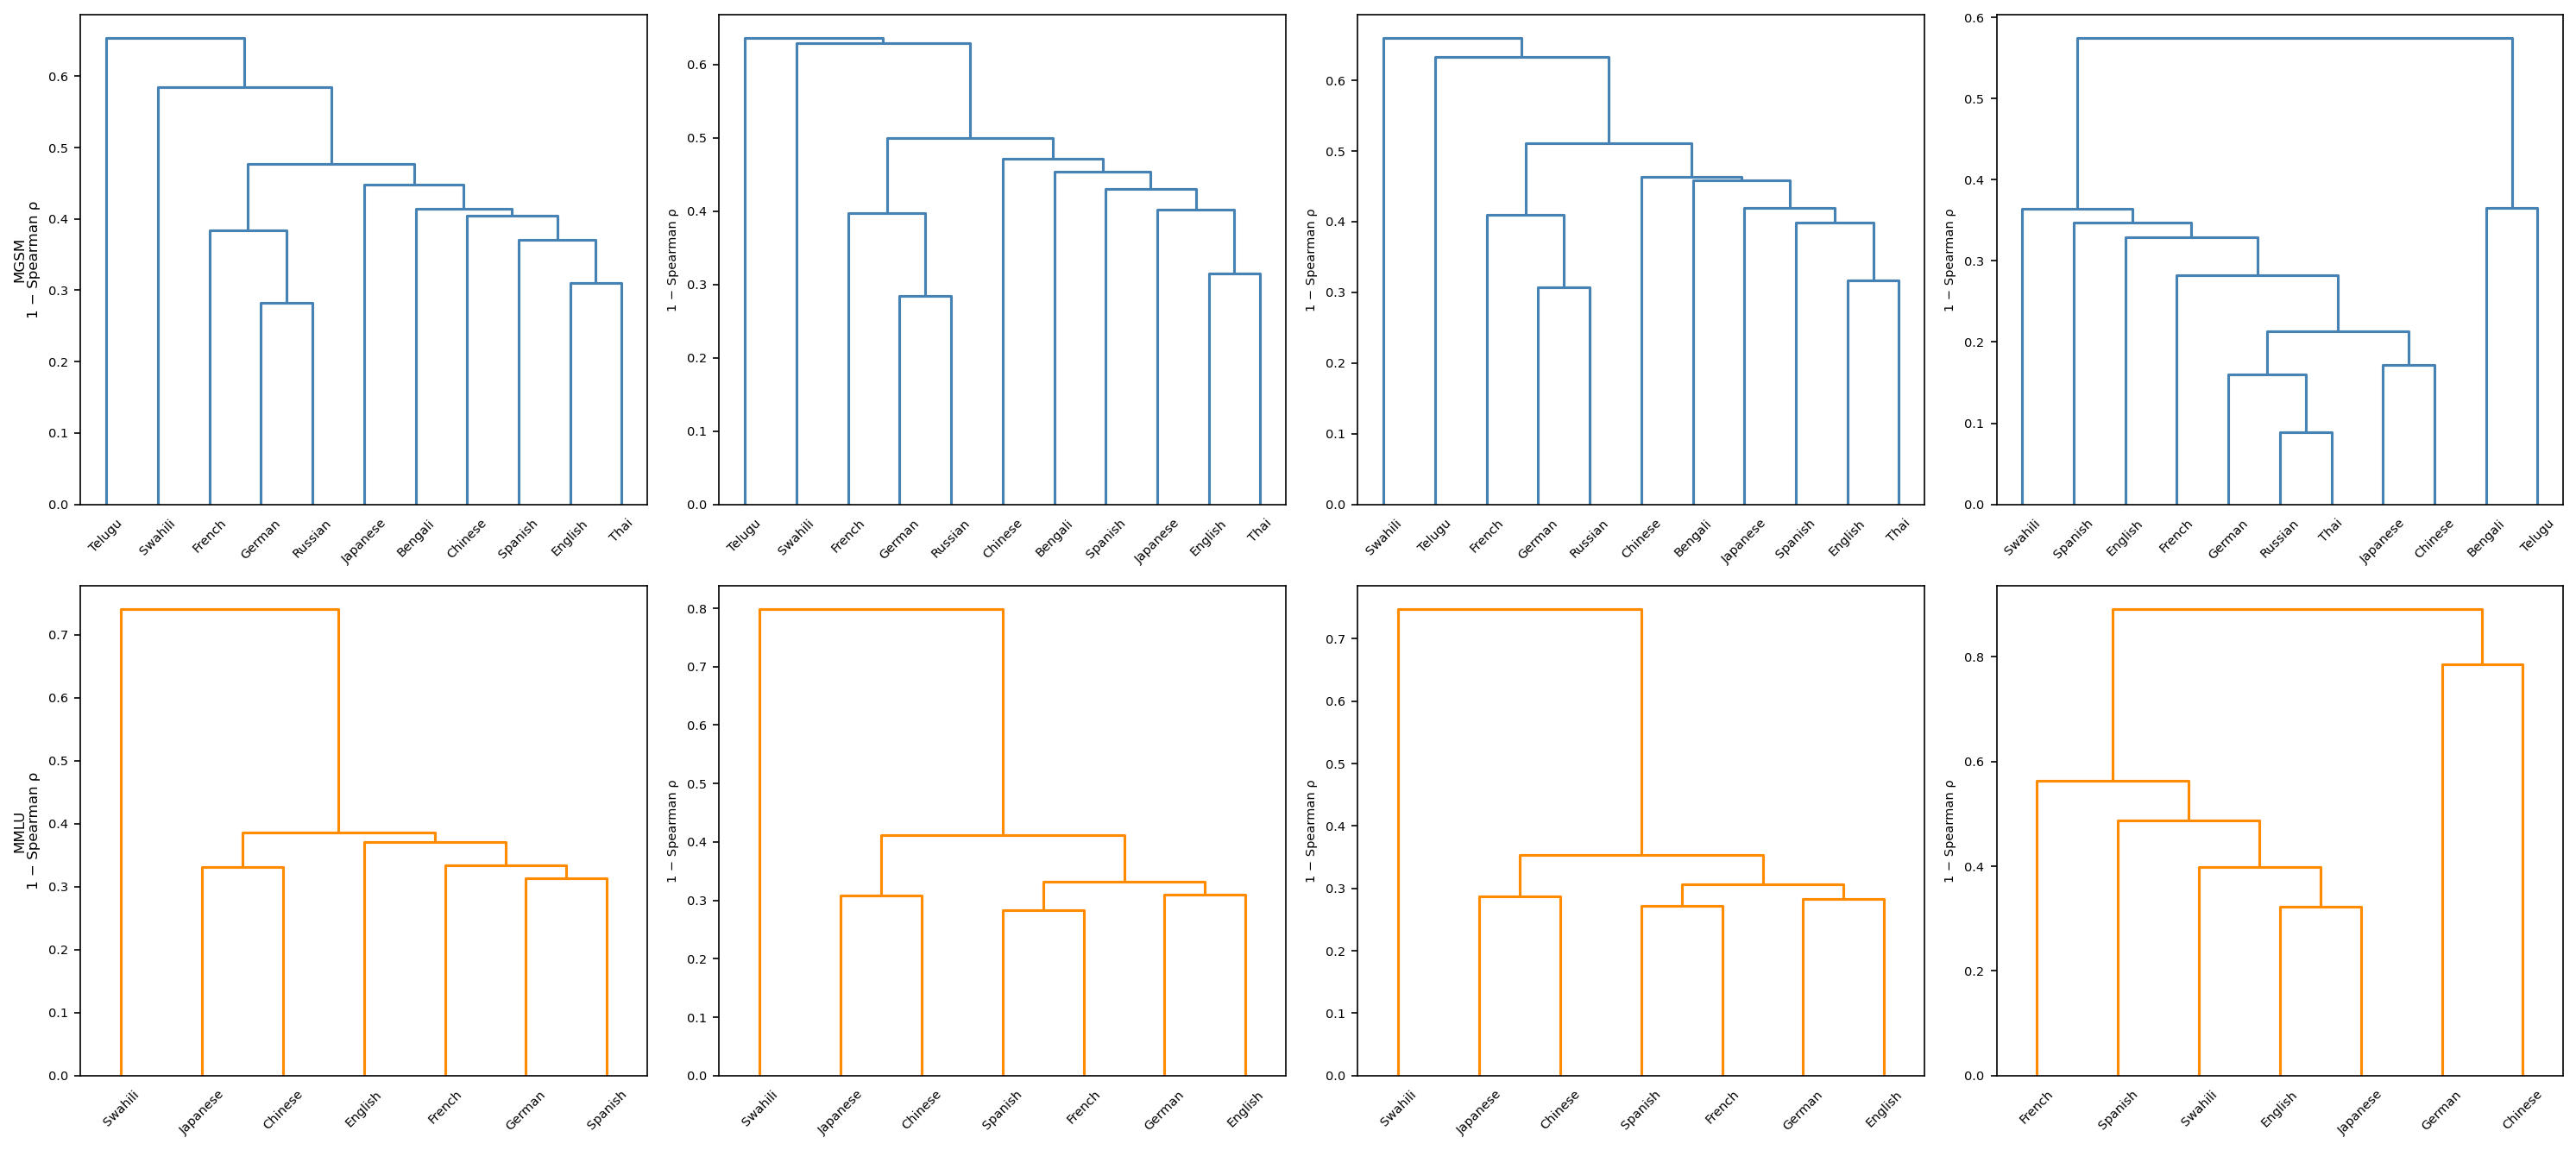
\includegraphics[width=\linewidth]{accuracy_irt_dendrograms}
  \caption{Language clustering by \textit{difficulty} for MGSM (top row) and MMLU (bottom row). Columns 1--3 cluster languages by pairwise Spearman correlation of item
    difficulty rank profiles under 1PL, 2PL, and 3PL respectively.
    Column 4 clusters languages by pairwise Spearman correlation of model
    accuracy vectors.}
  \label{fig:dendrograms}
\end{figure}

\begin{figure}[t]
  \centering
  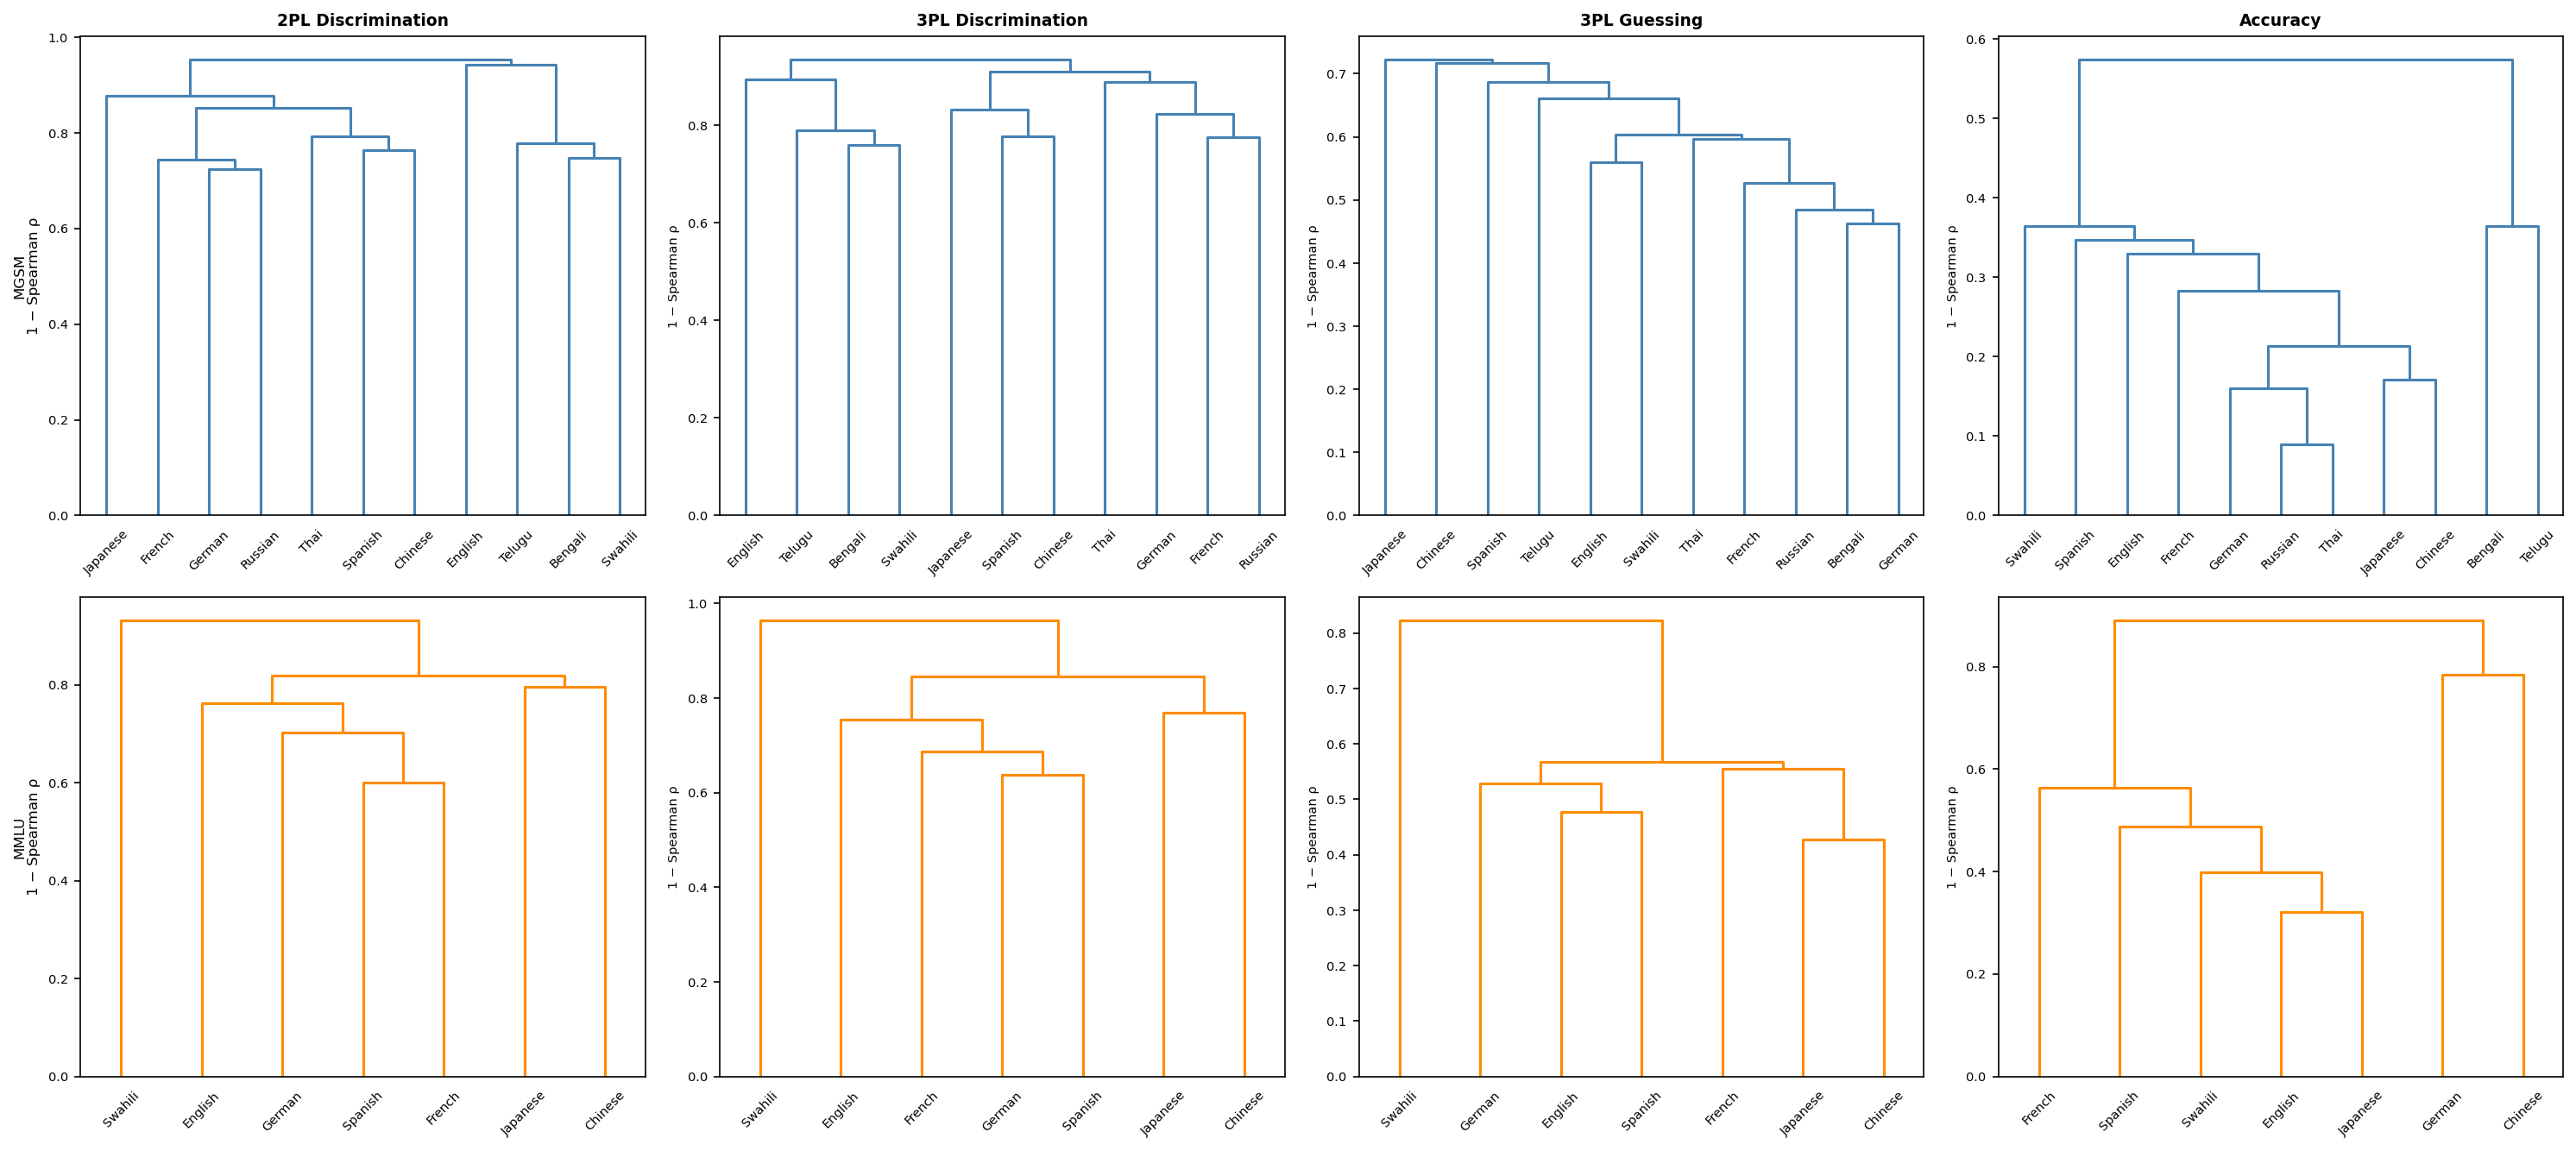
\includegraphics[width=\linewidth]{dendrograms_disc_guess}
  \caption{Language clustering by \textit{discrimination} (for 2PL and 3PL),
    and \textit{guessing }(3PL).Rows: MGSM (top), MMLU (bottom). Columns:
    2PL discrimination, 3PL discrimination, 3PL guessing, accuracy (left to right). }
  \label{fig:dendrograms_disc_guess}
\end{figure}

\paragraph{Language Clustering}
\label{sec:lang_clustering}

We cluster languages hierarchically (average linkage on Spearman distance $1-\rho$)
by each IRT parameter profile and compare to accuracy-based clusterings via Mantel
test and mean pairwise Spearman $\bar{\rho}$. For \textit{difficulty} (\autoref{fig:dendrograms}), MGSM dendrograms mirror the accuracy clustering: European languages cluster tightly while Telugu and Swahili are most isolated. A Mantel test quantifies alignment between each IRT difficulty clustering and the accuracy clustering (MGSM: 1PL $r = 0.63$, $p =0.001$; 2PL $r = 0.56$, $p = 0.002$; 3PL $r = 0.53$, $p = 0.003$; all MMLU tests non-significant). For MMLU, the accuracy dendrogram is structurally decoupled from IRT difficulty profiles where German and Chinese cluster as nearest neighbours despite typological distance, while Swahili clusters with European
languages in accuracy space, suggesting MMLU performance might be governed more by
pretraining data distribution than item difficulty structure.

For \textit{discrimination} and \textit{guessing}(\autoref{fig:dendrograms_disc_guess}),
the same procedure is applied with mean pairwise $\bar{\rho}$ as an additional
cross-lingual consistency measure. Discrimination is the least cross-lingually
consistent parameter ($\bar{\rho} \approx 0.10$ on both benchmarks), producing
near-equidistant clusterings with no interpretable structure; Mantel tests are
non-significant except MGSM 2PL discrimination ($r = 0.34$, $p = 0.005$), a signal
that disappears under 3PL. Guessing shows substantially higher cross-lingual
consistency ($\bar{\rho} \approx 0.35$ on both benchmarks), visible in lower and more
differentiated merge heights, but does not align with typological or accuracy-based
groupings (all Mantel tests non-significant). Thus, across all benchmarks and model
variants, \textit{difficulty} is the most consistent with being the only one showing accuracy alignment, but \textit{guessing} also recovers consistent interpretable
typological structure.

%We cluster languages hierarchically (average linkage on Spearman distance $1-\rho$) under each IRT variant and compare to a parallel clustering derived from model accuracy vectors, with a Mantel test quantifying alignment between the two structures (Figure~\ref{fig:dendrograms}). For MGSM, the 1PL dendrogram produces an interpretable grouping that closely mirrors the accuracy clustering: Telugu is the most isolated language, Swahili the second, European languages (French, German, Russian) form a tight low-distance cluster, and East/South Asian languages form a distinct group. The Mantel test confirms this alignment formally ($r = 0.63$, $p = 0.001$). Under 2PL and 3PL, the dendrogram collapses entirely — all merge heights inflate toward or beyond $1.0$, erasing any interpretable structure, and Mantel correlations drop to near zero — consistent with the instability of discrimination parameters shown above. For MMLU, no IRT model produces a clustering that aligns with accuracy (all Mantel tests non-significant). The 1PL dendrogram isolates Swahili clearly but otherwise shows little typological structure. The accuracy dendrogram is structurally unrelated to any IRT grouping: German and Chinese emerge as nearest neighbours despite typological distance, and Swahili — the most isolated language under every IRT model — clusters with European languages in the accuracy tree. This suggests MMLU accuracy might be governed by model pretraining data distribution rather than item-level difficulty structure, with high-resource language pairs co-occurring in training corpora pulling languages together in accuracy space regardless of their IRT profiles.

\subsection{Subset Analysis }
\label{sec:iif}



\paragraph{IIF Concordance}

We examine whether the three IRT variants agree on which items are most informative, a choice with direct consequences for the validity of any resulting cross-lingual subset (within-language fit comparisons are in \autoref{app:withinlangfits}). Agreement is operationalised via the Item Information Function (IIF) at $\theta=0$; a sensitivity analysis at $\theta \in \{-1, 0, +1\}$ confirms that the qualitative orderings are robust to this choice (\autoref{app:theta}): 
\begin{align}
  I_j^{(1\text{PL})} &= P_j\,(1 - P_j), \label{eq:iif1pl} \\
  I_j^{(2\text{PL})} &= a_j^2\, P_j\,(1 - P_j), \label{eq:iif2pl} \\
  I_j^{(3\text{PL})} &= \frac{a_j^2\,(P_j - c_j)^2\,(1 - P_j)}{(1-c_j)^2\,P_j},
  \label{eq:iif3pl}
\end{align}
where $b_j$, $a_j$, $c_j$ are difficulty, discrimination, and guessing
parameters; $P_j^{(1\text{PL})} = \sigma(-b_j)$;
$P_j^{(2\text{PL})} = \sigma(a_j(-b_j))$;
$P_j^{(3\text{PL})} = c_j + (1-c_j)\,\sigma(a_j(-b_j))$.
Per slice, items are ranked by $I_j$ and the top 50\% retained
(avg.\ 125 items per MGSM slice; 33 per MMLU slice; sensitivity to this threshold in \autoref{app:compression}); pairwise agreement is
measured by Jaccard similarity $J(A,B) = |A \cap B|/|A \cup B|$, with an
expected baseline of $J \approx 0.33$ for two independent random draws
(\autoref{fig:iif_concordance}).Across both benchmarks, 1PL--2PL agreement (median $J = 0.40$ for MGSM, $J = 0.53$ for MMLU) and 1PL--3PL (median $J = 0.41$ for MGSM, $J = 0.45$ for MMLU) both exceed the random-selection baseline ($J \approx 0.33$). 2PL--3PL shows the strongest concordance overall (median $J = 0.92$ for MGSM, $J = 0.59$ for MMLU), confirming that 2PL and 3PL agree very strongly with each other on which items are most informative. MMLU shows lower 2PL--3PL concordance, reflecting greater variation across the heterogeneous domain slices. 

\begin{figure}[t]
  \centering
  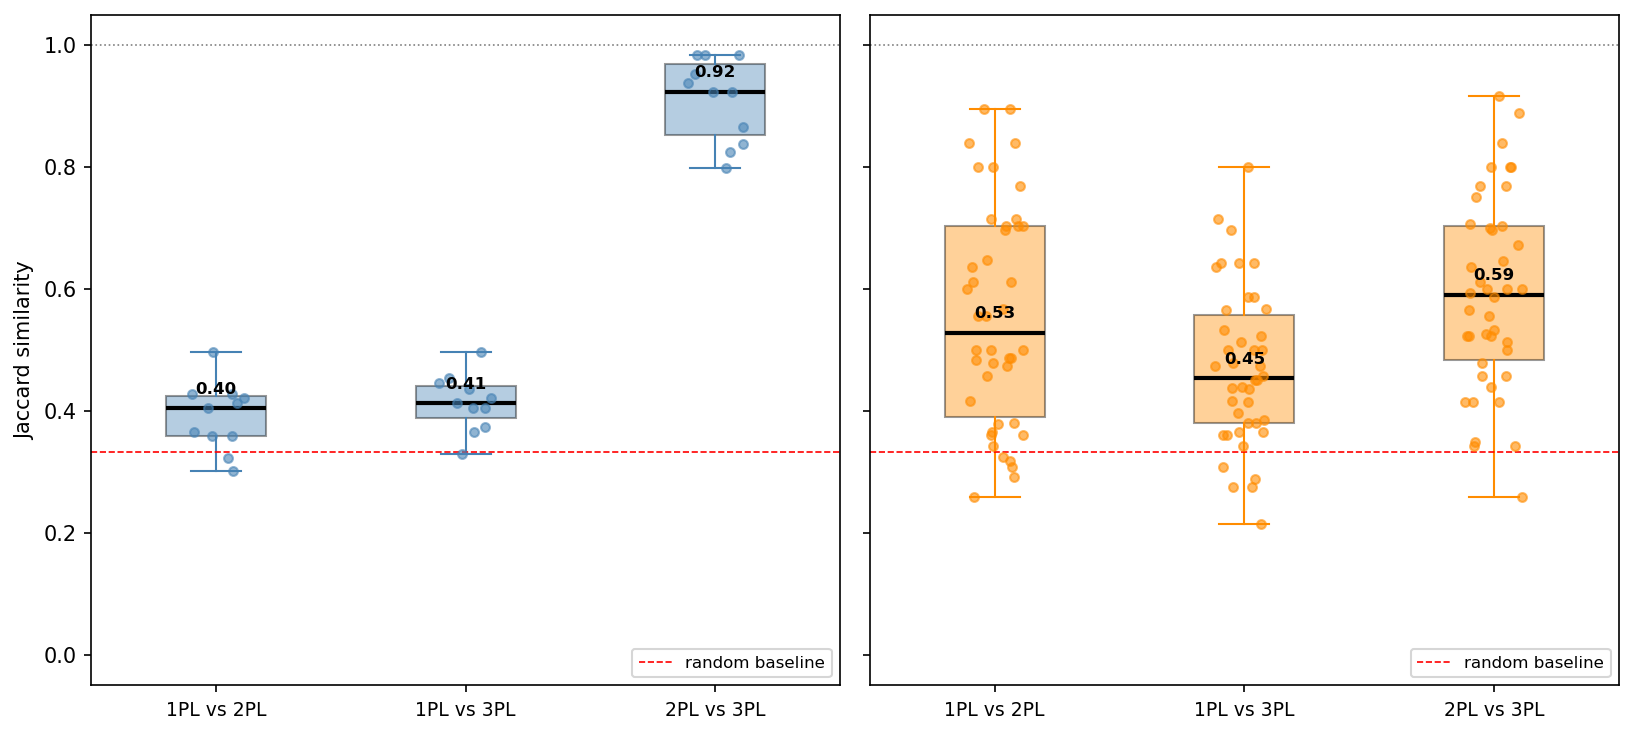
\includegraphics[width=\linewidth]{iif_concordance}
  \caption{Jaccard similarity of the top-50\% items selected by IIF at $\theta=0$ for each model pair \textbf{(left: MGSM; right: MMLU)}, across all benchmark slices (11 MGSM languages; 42 MMLU language$\times$domain combinations). Each dot is one slice; annotated values are medians. Dashed line marks the random-selection baseline ($J \approx 0.33$).}
  \label{fig:iif_concordance}
\end{figure}

Thus, switching from 1PL to 2PL or 3PL modifies item selection but does not discard all shared signal, with 2PL and 3PL producing closely related subsets. The low 1PL--2PL/3PL concordance reflects that 1PL selects items by difficulty alone, while 2PL and 3PL IIFs are dominated by the discrimination term, prioritising different, and more language-idiosyncratic, items. The strong 2PL--3PL concordance on MGSM ($J = 0.92$) reflects near-zero guessing rates on open-ended math items, so the guessing correction in 3PL barely shifts selection from 2PL; the lower concordance on MMLU ($J = 0.59$) confirms that guessing becomes consequential for multiple-choice items where chance-level correctness is non-negligible.


\begin{figure}[t]
  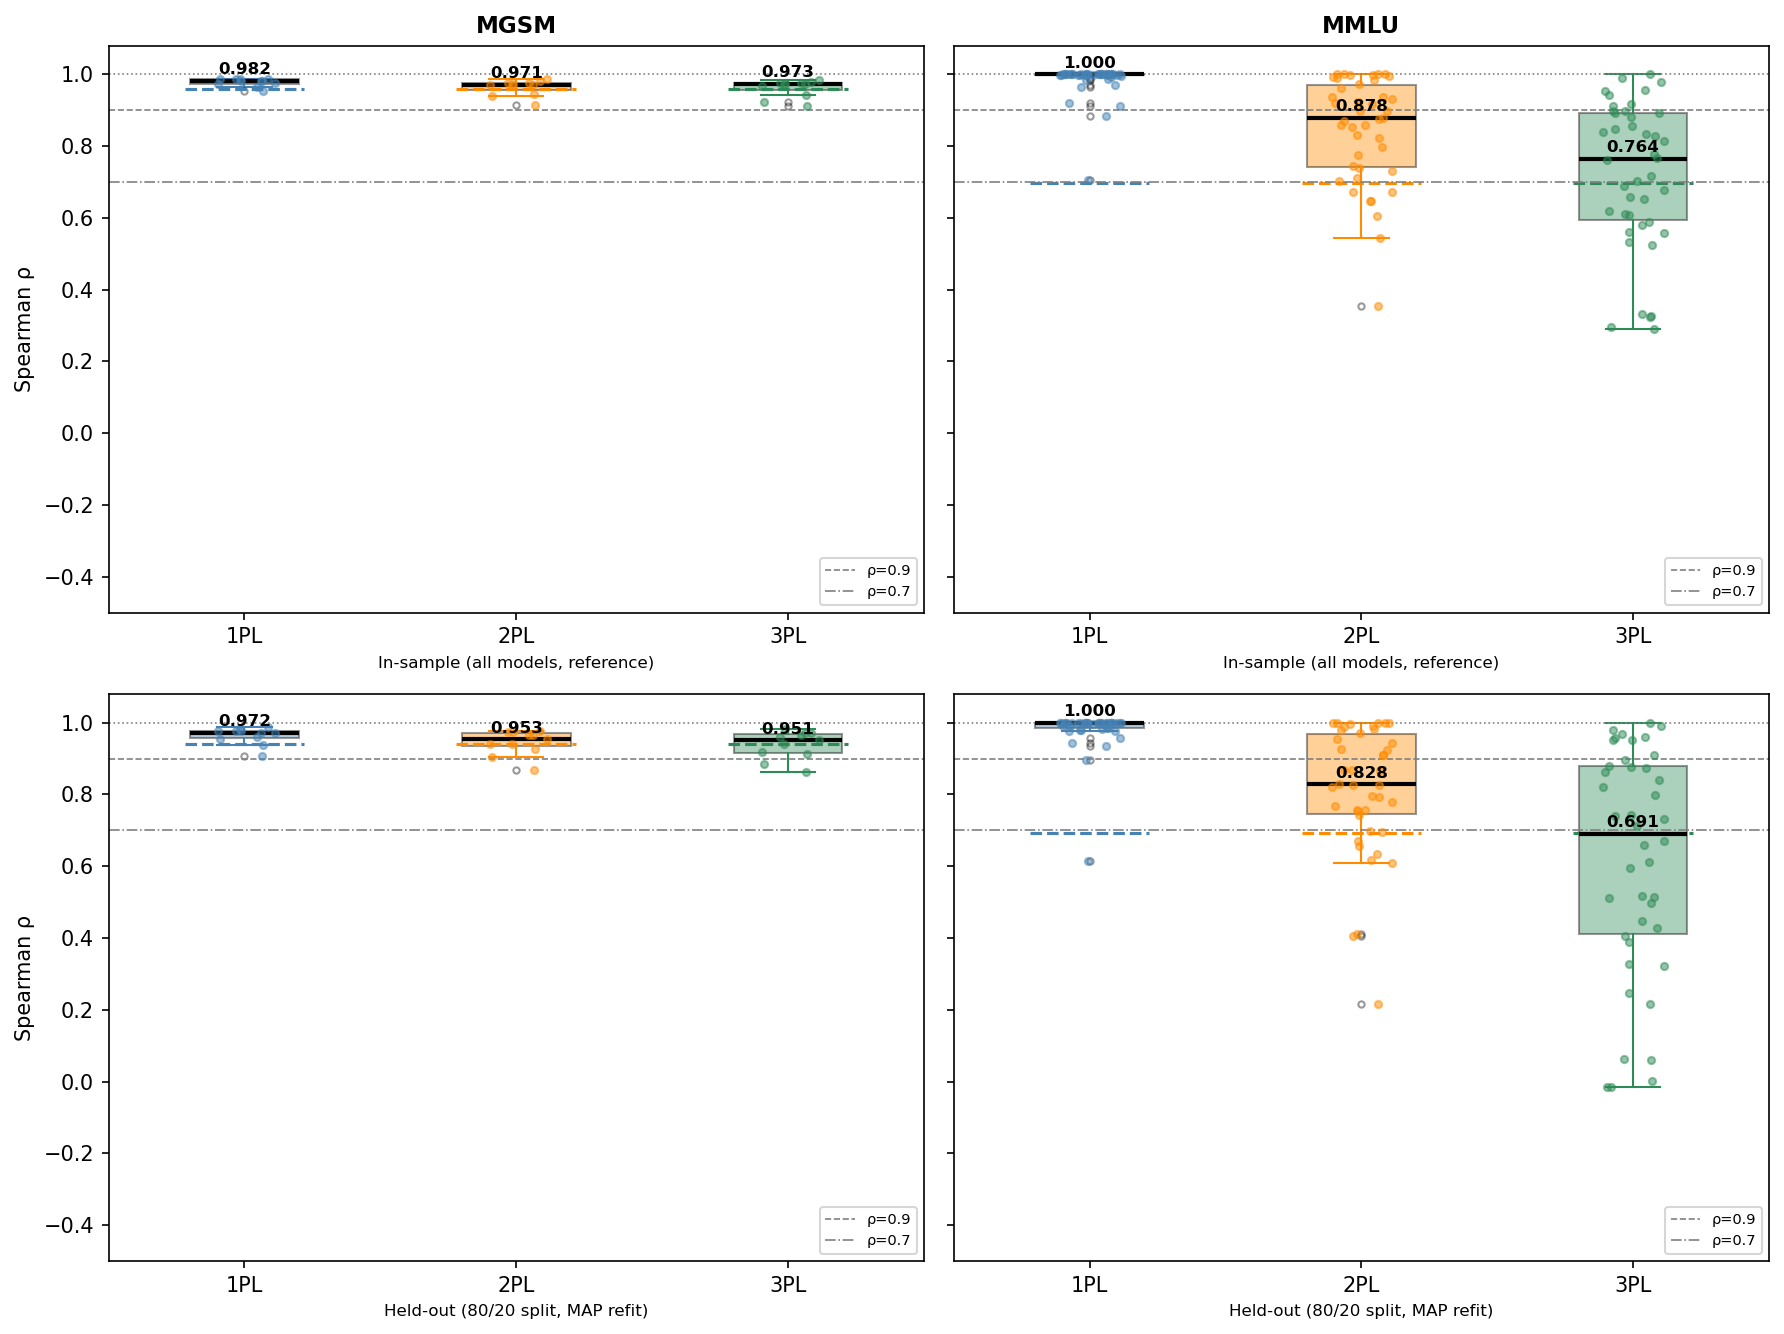
\includegraphics[width=\linewidth]{images_2/heldout_vs_insample_map.png}
  \caption{Ranking fidelity (Spearman $\rho$, subset vs.\ full benchmark) for MGSM
    (left) and MMLU (right). \textbf{Top row}: in-sample (all models, upper bound).
    \textbf{Bottom row}: held-out (IRT re-fitted on 80\% of models, evaluated on
    remaining 20\%). Dashed line marks the random-item baseline. 1PL fidelity is stable across both splits.}
  \label{fig:heldout_vs_insample}
\end{figure}


\paragraph{Ranking Fidelity}

\begin{table}[t]
  \centering
  \resizebox{\columnwidth}{!}{%
  \begin{tabular}{lcccc}
    \toprule
    & \multicolumn{2}{c}{\textbf{MGSM}} & \multicolumn{2}{c}{\textbf{MMLU}} \\
    \cmidrule(lr){2-3}\cmidrule(lr){4-5}
    \textbf{Selection strategy} & In-samp. & Held-out & In-samp. & Held-out \\
    \midrule
    1PL (difficulty)            & 0.982 & 0.972 & 1.000 & 1.000 \\
    2PL difficulty only         & 0.978 & 0.970 & 0.932 & 0.932 \\
    2PL (diff$+$disc)     & 0.971 & 0.953 & 0.878 & 0.831 \\
    3PL difficulty only         & 0.979 & 0.972 & 0.922 & 0.889 \\
    3PL (diff $+$ disc)           & 0.975 & 0.950 & 0.850 & 0.778 \\
    3PL (diff $+$ disc$+$ guess)    & 0.973 & 0.951 & 0.764 & 0.691 \\
    \bottomrule
  \end{tabular}}
  \caption{Median Spearman $\rho$ (subset vs.\ full benchmark) under progressively
    richer IIF selection strategies; the gap between rows isolates that
    parameter's marginal contribution to fidelity loss.}
  \label{tab:param_decomp}
\end{table}


Since IIF concordance shows that IRT model choice determines which items are selected,
we now ask whether those selections preserve \emph{model rankings} on the full
benchmark. We evaluate four conditions: (i)~in-sample same-language; (ii)~held-out
same-language (IRT fitted on 80\% of models, evaluated on held-out 20\%);
(iii)~in-sample cross-lingual; and (iv)~held-out cross-lingual. The primary metric is
Spearman $\rho$ between per-model subset accuracy and full-benchmark accuracy,
compared against a 200-draw random-item baseline (\autoref{fig:heldout_vs_insample}). Under 1PL, same-language fidelity is high and stable across both splits: in-sample median $\rho = 0.982$ (MGSM) and $1.000$ (MMLU), dropping only marginally on held-out models ($0.972$ and $1.000$), well above the random baselines. On MGSM, 2PL and 3PL also preserve strong held-out fidelity ($\rho = 0.953$ and $0.951$), showing that with stable parameter estimation all three variants are viable. On MMLU, fidelity degrades progressively with model complexity: 2PL held-out median $\rho = 0.828$ and 3PL $\rho = 0.691$, with 3PL showing the widest spread and several low-fidelity slices (per-slice distributions and accuracy scatter plots in Appendix~\ref{app:ranking_fidelity}).

To isolate which parameter drives this degradation, \autoref{tab:param_decomp}
decomposes fidelity by applying progressively richer IIF formulas, also shown in \autoref{fig:param_decomp}: on MGSM all six strategies yield near-identical fidelity, confirming that difficulty alone drives the signal; on MMLU fidelity drops monotonically with each parameter added, with discrimination causing the largest single step down. Selecting items by \textit{difficulty alone} preserves high fidelity across both benchmarks regardless of which PL model fitted it (MGSM held-out: $\rho \approx 0.97$; MMLU held-out: $0.89$--$0.93$). Adding \textit{discrimination} introduces the primary degradation: $-0.017$--$0.022$ on MGSM and $-0.101$--$0.111$ on MMLU held-out, consistent with discrimination being language-idiosyncratic. Adding \textit{guessing} further reduces MMLU held-out fidelity by $0.087$ ($0.778 \to 0.691$) while leaving MGSM virtually unchanged ($0.950 \to 0.951$). Together, it is not model complexity per se but the \textit{discrimination} parameter that drives fidelity loss, and difficulty-based or 1PL selection remains the safest cross-lingual strategy.



\begin{figure}[t]
  \centering
  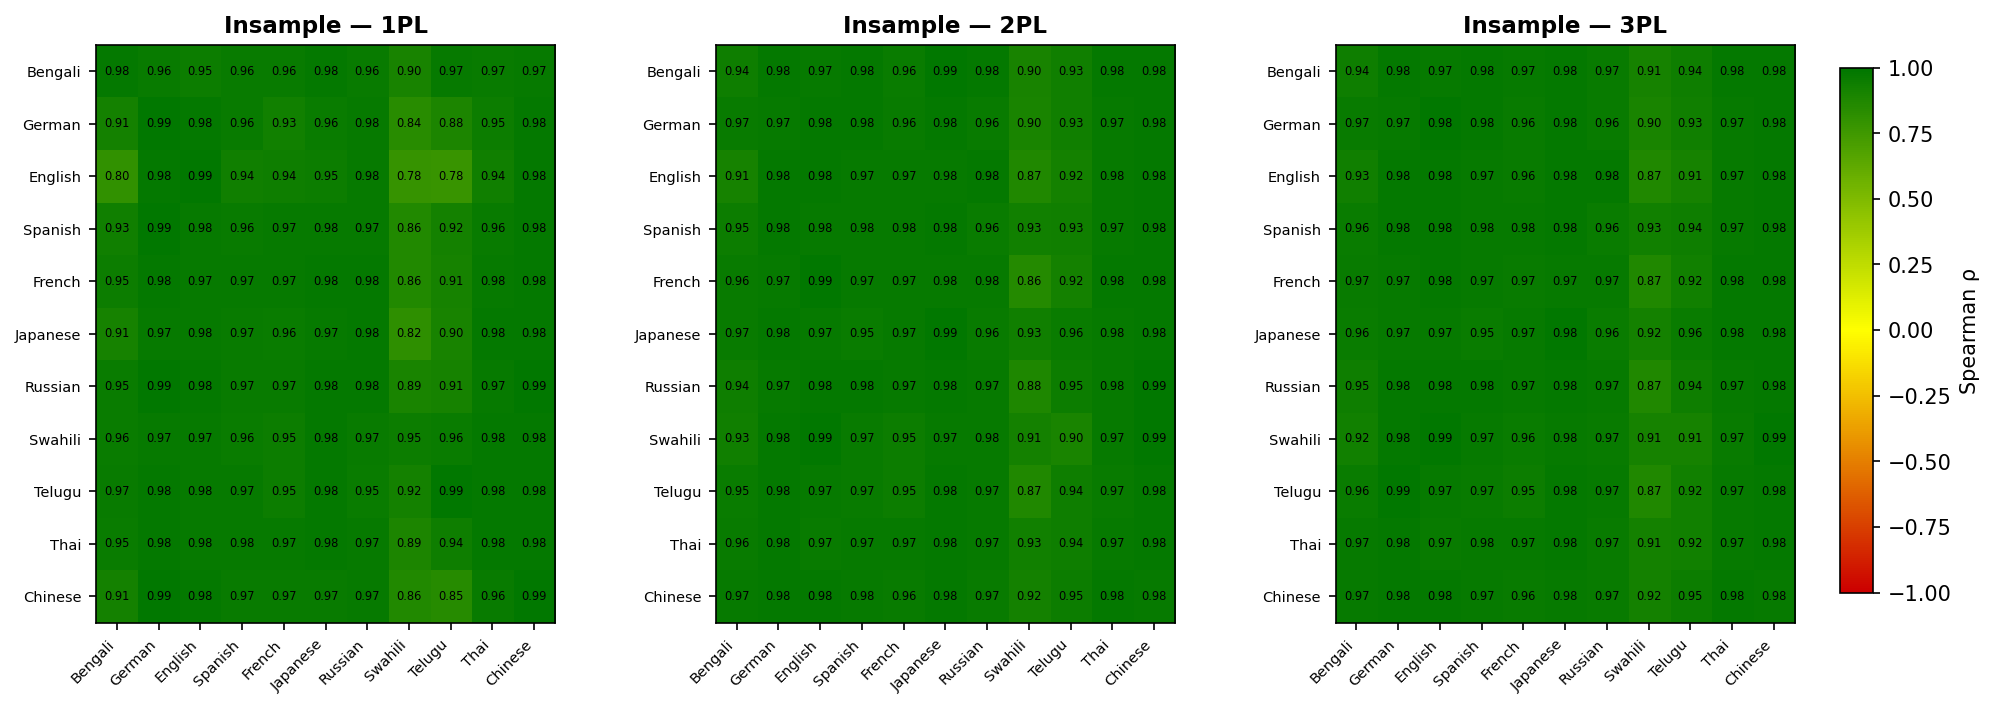
\includegraphics[width=\columnwidth]{images_2/crosslingual_insample_mgsm}\\[2pt]
  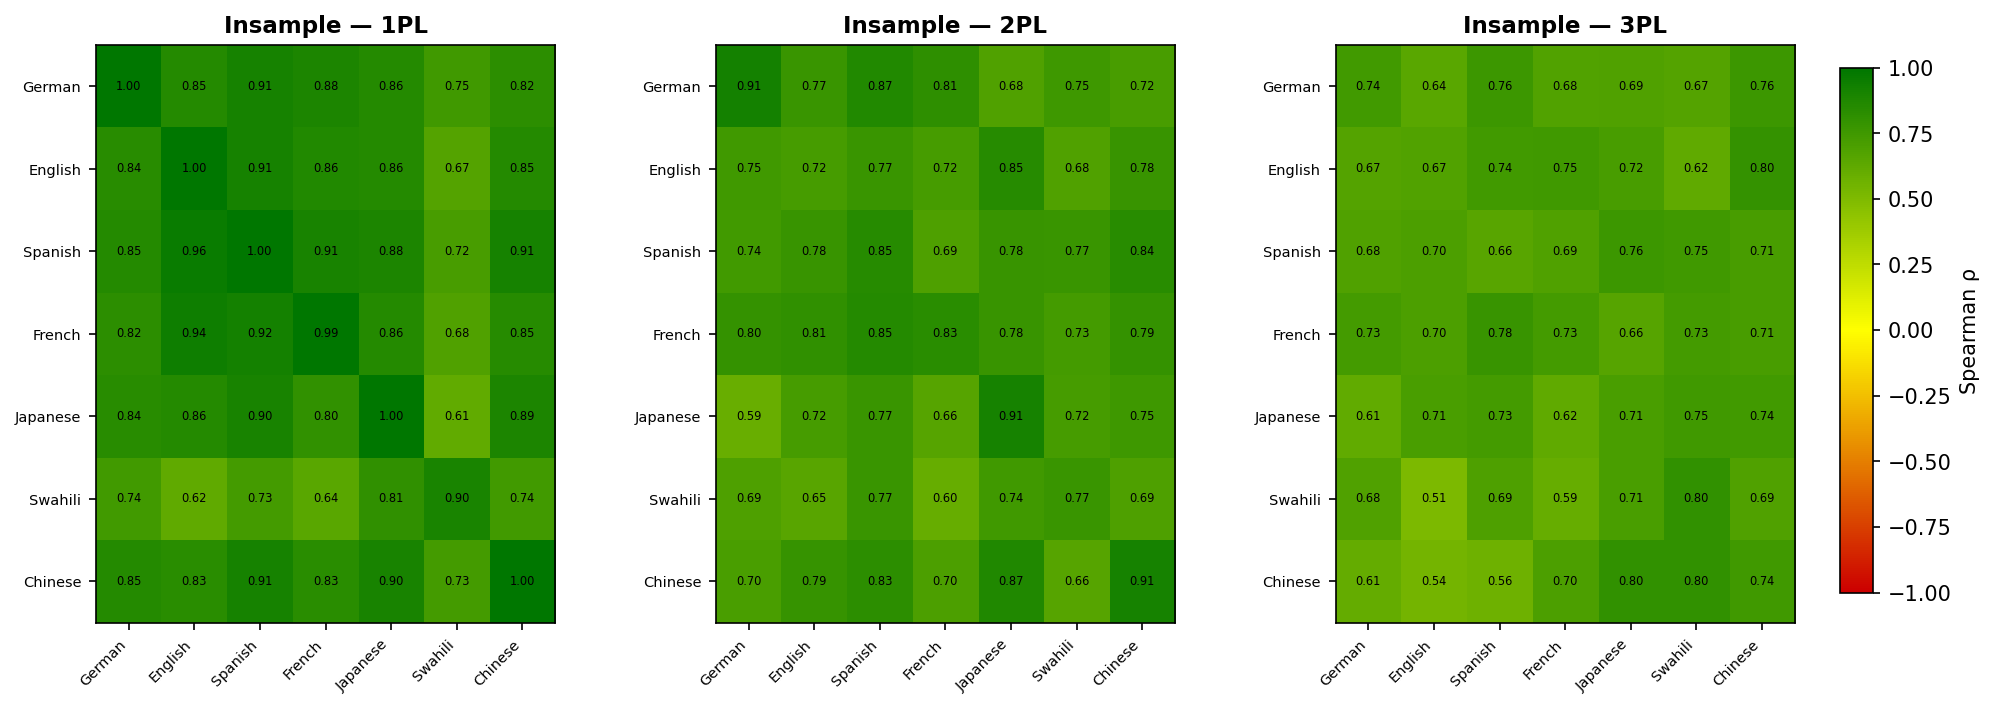
\includegraphics[width=\columnwidth]{images_2/crosslingual_insample_mmlu}
  \caption{In-sample cross-lingual subset ranking fidelity. Cell $(i,j)$ is Spearman
    $\rho$ between subset accuracy (items from language $i$) and full-benchmark
    accuracy in language $j$. \textbf{Top:} MGSM. \textbf{Bottom:} MMLU (avg.\ over six domains). Columns = 1PL, 2PL, 3PL.}
  \label{fig:crosslang_insample}
\end{figure}

\begin{figure}[t]
  \centering
  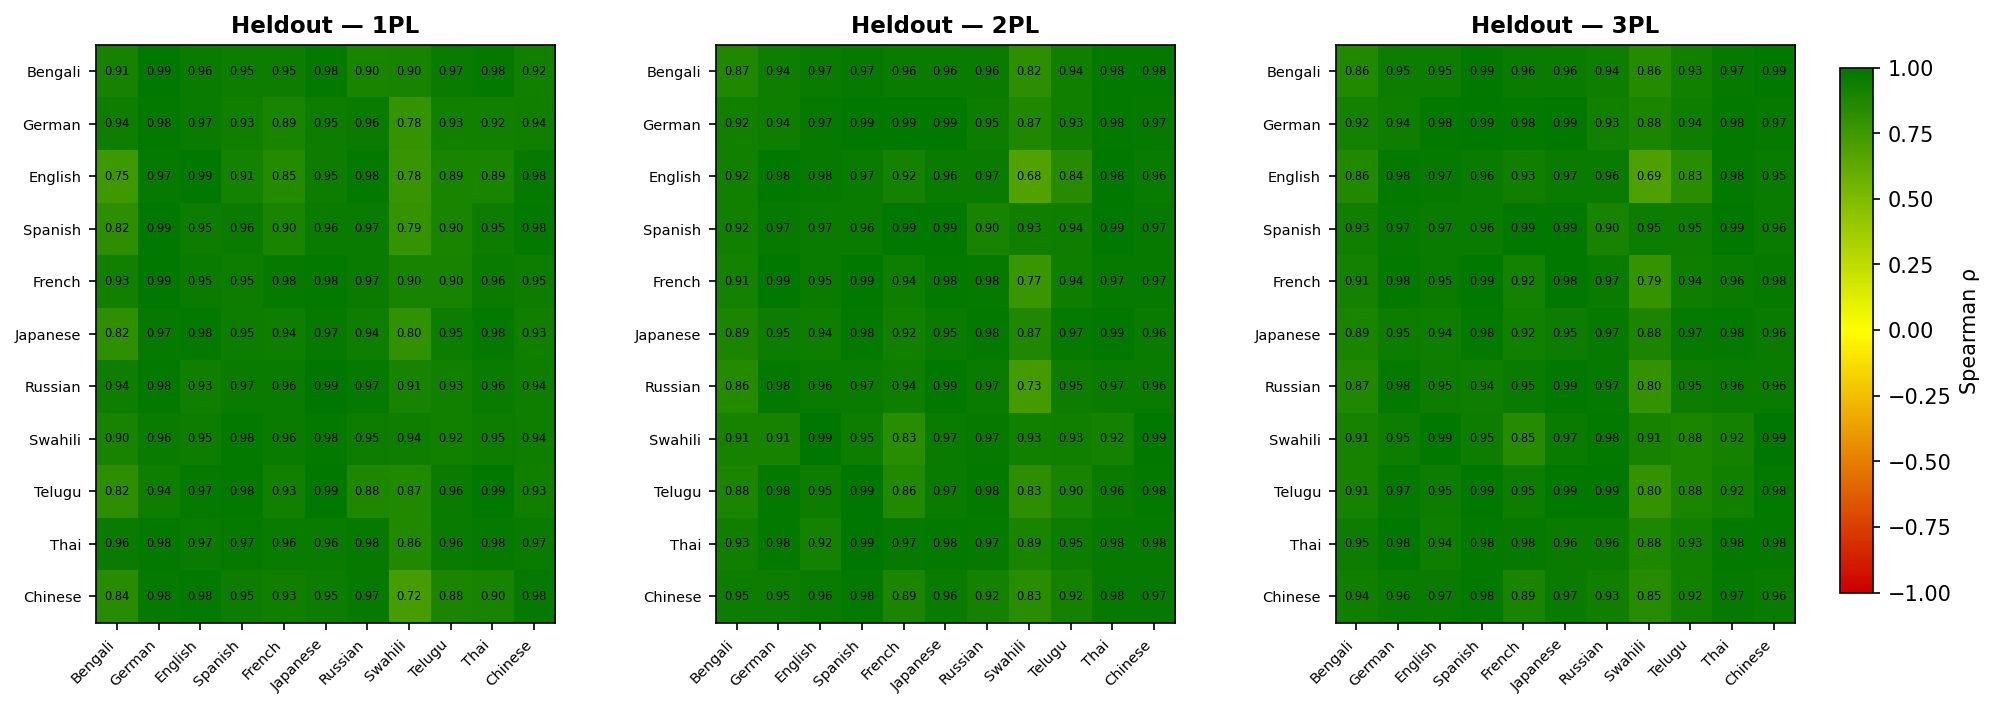
\includegraphics[width=\columnwidth]{images_2/crosslingual_heldout_mgsm}\\[2pt]
  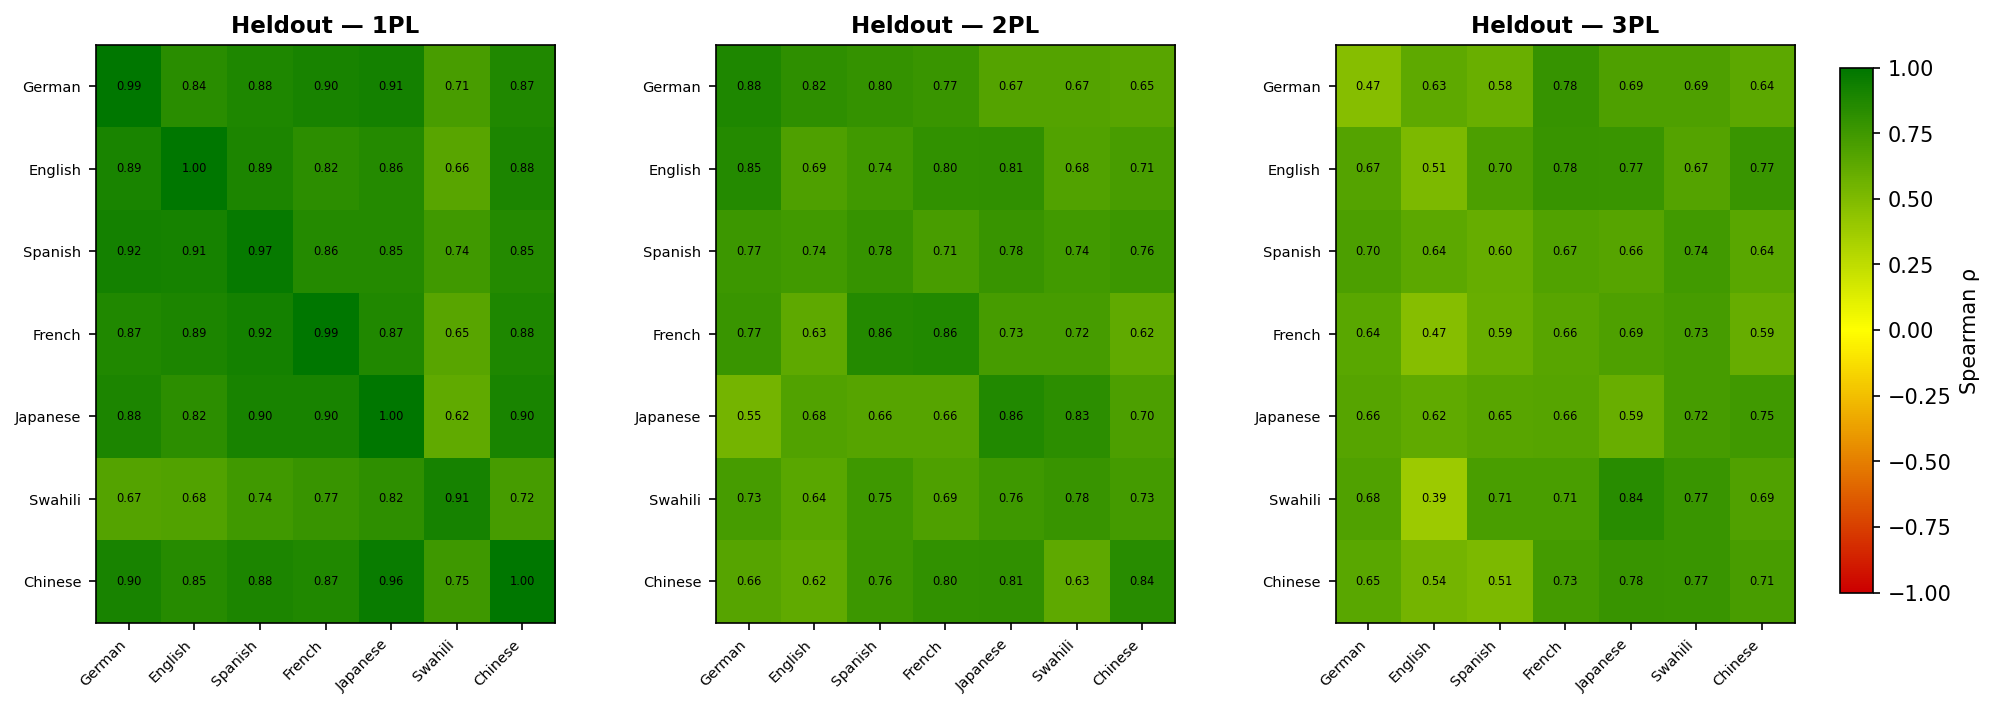
\includegraphics[width=\columnwidth]{images_2/crosslingual_heldout_mmlu}
  \caption{Held-out cross-lingual subset ranking fidelity (IRT re-fitted on 80\%
    of models via MAP, evaluated on 20\%). Same layout as
    Figure~\ref{fig:crosslang_insample}.}
  \label{fig:crosslang_heldout}
\end{figure}

\begin{table}[t]
  \centering
  \resizebox{\columnwidth}{!}{%
  \begin{tabular}{lcccc}
    \toprule
    & \multicolumn{2}{c}{\textbf{MGSM}} & \multicolumn{2}{c}{\textbf{MMLU}} \\
    \cmidrule(lr){2-3}\cmidrule(lr){4-5}
    \textbf{Selection strategy} & In-samp. & Held-out & In-samp. & Held-out \\
    \midrule
    1PL (difficulty)          & 0.968 & 0.949 & 0.854 & 0.877 \\
    2PL difficulty only       & 0.973 & 0.960 & 0.789 & 0.795 \\
    2PL (diff$+$disc)         & 0.973 & 0.962 & 0.765 & 0.777 \\
    3PL difficulty only       & 0.974 & 0.961 & 0.778 & 0.787 \\
    3PL (diff$+$disc)         & 0.972 & 0.958 & 0.761 & 0.749 \\
    3PL (diff$+$disc$+$guess) & 0.972 & 0.959 & 0.714 & 0.729 \\
    \bottomrule
  \end{tabular}}
  \caption{Median cross-lingual Spearman $\rho$ (off-diagonal pairs) under
    progressively richer IIF selection strategies. Items are selected using
    the source language IRT; fidelity is evaluated in the target language.}
  \label{tab:crosslingual_decomp}
\end{table}

\begin{figure}[t]
  \centering
  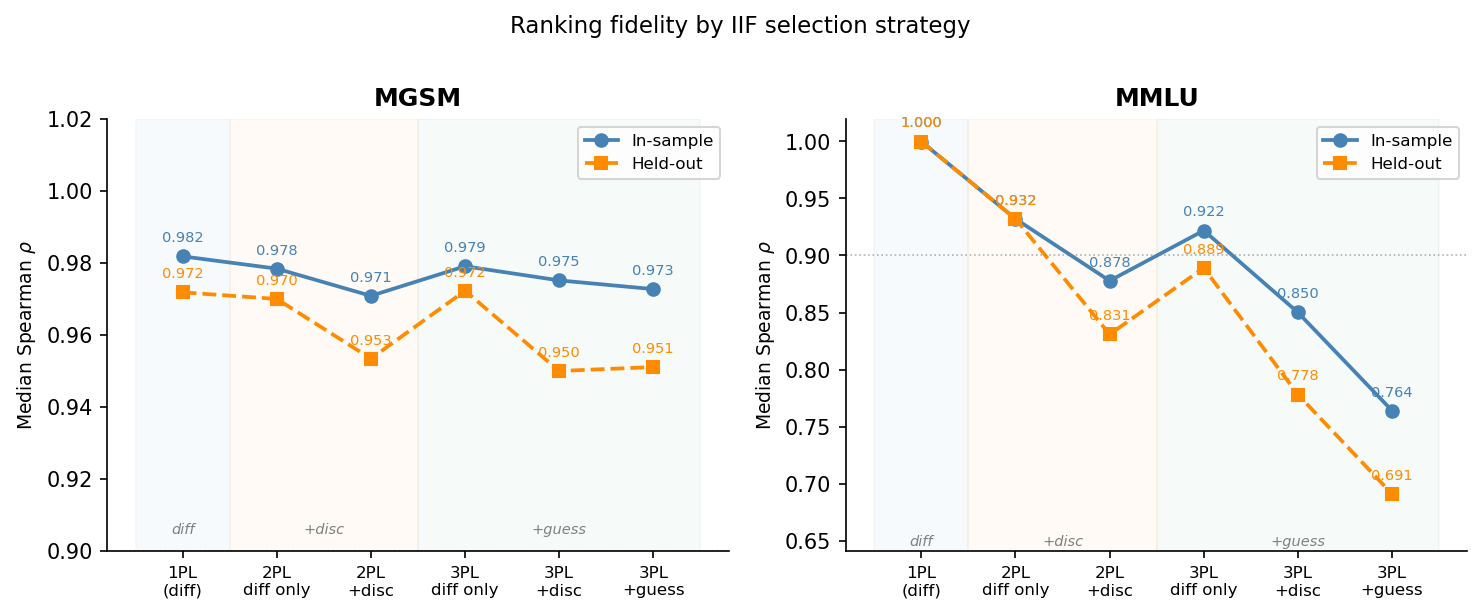
\includegraphics[width=\columnwidth]{images_2/param_decomposition}
  \caption{Median Spearman $\rho$ under progressively richer IIF selection
  strategies, isolating each parameter's marginal contribution to fidelity.}
  \label{fig:param_decomp}
\end{figure}



Cross-lingual transfer is shown in \autoref{fig:crosslang_insample} (insample) and \autoref{fig:crosslang_heldout} (heldout), with a parameter-wise decomposition in Table~\ref{tab:crosslingual_decomp}.On MGSM, all three variants transfer well (held-out median $\rho = 0.949$--$0.962$), with 2PL and 3PL matching or slightly exceeding 1PL: arithmetic difficulty is translation-invariant and discrimination adds negligible noise. On MMLU, 1PL is the only reliable cross-lingual variant (held-out $\rho = 0.877$); fidelity degrades steadily with model complexity (2PL: $0.777$; 3PL: $0.729$). The parameter decomposition reveals that discrimination drives this drop and switching to 2PL difficulty alone already costs $-0.082$ due to contamination from joint estimation with a language-specific discrimination parameter, with discrimination itself adding a further $-0.018$--$0.038$ penalty. Guessing contributes an additional but smaller $-0.020$ loss.  Inspecting the language-pair breakdown in the figures, this degradation is not uniform: Swahili is consistently the most isolated source and target, mirroring its outlier status in the concordance analysis (\S\ref{sec:cross_lingual}).




\section{Discussion}
\label{sec:analysis}

Across our two experiments, the findings converge on the same story.

\textbf{Cross-lingual concordance.} We find that difficulty is consistently the most stable IRT parameter across languages, and this concordance is maintained when we move to 2PL and 3PL difficulty estimates. Discrimination is different and substantially below difficulty across all variants and both benchmarks. Guessing sits between the two. The language clustering results reinforce this: on MGSM, difficulty profiles from all three models significantly track language typology, while discrimination profiles do not. Additionally, STEM domains are consistently more concordant than humanities and social sciences across all variants, suggesting that reasoning-based items are more translation-stable than culturally situated ones.

\textbf{Subset analysis.} Within-language, 1PL subsets preserve model rankings reliably on both benchmarks, and 2PL and 3PL are competitive on MGSM but degrade substantially on MMLU. Cross-lingually, MGSM remains robust across all three variants, while on MMLU 1PL is the only reliable variant. The parameter decomposition in Table~\ref{tab:crosslingual_decomp} shows that most of the fidelity drop happens before discrimination even enters selection: switching from 1PL to 2PL difficulty alone already costs substantial fidelity on MMLU.

Together, these results reflect something fundamental about what each IRT parameter captures. Difficulty measures how hard an item is for the average model: a property that, for a well-translated item, should survive translation. Discrimination measures how sharply an item separates strong from weak models, which depends on how capabilities distribute in that language and on surface features of the item's phrasing neither of which is translation-invariant. Guessing reflects how often models answer correctly at chance, mediated by pretraining knowledge; since pretraining exposure is uneven but not entirely language-specific, it holds up better than discrimination but not as well as difficulty.  More concretely, for using IRT filtering on multilingual translated benchmarks: i)we must not assume that a subset which works well within one language will generalise to others i.e.,  cross-lingual validity should be verified explicitly by checking concordance across typologically distant languages before deployment and ii) we must account for domain composition as science and STEM domains are reliably more cross-lingually stable than humanities and social sciences, and a single overall fidelity check will mask important variation within mixed-domain benchmarks. Model complexity should match to the stability of the data since richer IRT models are not always better, and when cross-lingual concordance is limited, simpler models that rely only on the most stable parameters will produce more transferable subsets.



\section{Conclusion}

We set out to test a basic but largely unexamined assumption in multilingual LLM evaluation: that IRT, an established tool for benchmark filtering, behaves consistently when the same benchmark is translated across languages. The answer is that it does but only for some parameters. Difficulty is moderately stable across languages for all IRT variants and both benchmark types, and IRT-filtered subsets built from one language reliably preserve model rankings in another. Discrimination does not transfer: it captures language-specific rather than item-specific signal, and Guessing sits between the two, reflecting pretraining-mediated chance performance rather than language-specific item structure. This parameter hierarchy is consistent across concordance measures, language clustering, and subset ranking fidelity, and it determines a clear practical recommendation: 1PL is the most reliable cross-lingual variant. However,our conclusions are grounded in open-weight instruction-tuned models under 20
billion parameters and a language sample skewed toward European languages; their
scope should be verified before extension to frontier models or typologically distant
language families not represented here. 


As translation-based multilingual benchmarks become standard infrastructure for LLM evaluation, the psychometric properties of translated items cannot be assumed to carry over across languages. Our findings show that the choice of IRT model and the stability of its parameters are not incidental details: they determine whether a compressed benchmark remains valid across the languages it is meant to evaluate. Cross-lingual validity should be demonstrated, not assumed, and we hope this work provides a concrete empirical basis for that standard.


%We hope this motivates further work on psychometrically grounded criteria for multilingual benchmark construction and validation.We hope this motivates further work on psychometrically grounded multilingual evaluation, and principled criteria for when language-specific calibration is warranted for evaluation benchmarks.

\begin{comment}


\section{Introduction}

These instructions are for authors submitting papers to *ACL conferences using \LaTeX. They are not self-contained. All authors must follow the general instructions for *ACL proceedings,\footnote{\url{http://acl-org.github.io/ACLPUB/formatting.html}} and this document contains additional instructions for the \LaTeX{} style files.

The templates include the \LaTeX{} source of this document (\texttt{acl\_latex.tex}),
the \LaTeX{} style file used to format it (\texttt{acl.sty}),
an ACL bibliography style (\texttt{acl\_natbib.bst}),
an example bibliography (\texttt{custom.bib}),
and the bibliography for the ACL Anthology (\texttt{anthology.bib}).

\section{Engines}

To produce a PDF file, pdf\LaTeX{} is strongly recommended (over original \LaTeX{} plus dvips+ps2pdf or dvipdf).
The style file \texttt{acl.sty} can also be used with
lua\LaTeX{} and
Xe\LaTeX{}, which are especially suitable for text in non-Latin scripts.
The file \texttt{acl\_lualatex.tex} in this repository provides
an example of how to use \texttt{acl.sty} with either
lua\LaTeX{} or
Xe\LaTeX{}.

\section{Preamble}

The first line of the file must be
\begin{quote}
\begin{verbatim}
\documentclass[11pt]{article}
\end{verbatim}
\end{quote}

To load the style file in the review version:
\begin{quote}
\begin{verbatim}
\usepackage[review]{acl}
\end{verbatim}
\end{quote}
For the final version, omit the \verb|review| option:
\begin{quote}
\begin{verbatim}
\usepackage{acl}
\end{verbatim}
\end{quote}

To use Times Roman, put the following in the preamble:
\begin{quote}
\begin{verbatim}
\usepackage{times}
\end{verbatim}
\end{quote}
(Alternatives like txfonts or newtx are also acceptable.)

Please see the \LaTeX{} source of this document for comments on other packages that may be useful.

Set the title and author using \verb|\title| and \verb|\author|. Within the author list, format multiple authors using \verb|\and| and \verb|\And| and \verb|\AND|; please see the \LaTeX{} source for examples.

By default, the box containing the title and author names is set to the minimum of 5 cm. If you need more space, include the following in the preamble:
\begin{quote}
\begin{verbatim}
\setlength\titlebox{<dim>}
\end{verbatim}
\end{quote}
where \verb|<dim>| is replaced with a length. Do not set this length smaller than 5 cm.

\section{Document Body}

\subsection{Footnotes}

Footnotes are inserted with the \verb|\footnote| command.\footnote{This is a footnote.}

\subsection{Tables and figures}

See Table~\ref{tab:accents} for an example of a table and its caption.
\textbf{Do not override the default caption sizes.}

\begin{table}
  \centering
  \begin{tabular}{lc}
    \hline
    \textbf{Command} & \textbf{Output} \\
    \hline
    \verb|{\"a}|     & {\"a}           \\
    \verb|{\^e}|     & {\^e}           \\
    \verb|{\`i}|     & {\`i}           \\
    \verb|{\.I}|     & {\.I}           \\
    \verb|{\o}|      & {\o}            \\
    \verb|{\'u}|     & {\'u}           \\
    \verb|{\aa}|     & {\aa}           \\\hline
  \end{tabular}
  \begin{tabular}{lc}
    \hline
    \textbf{Command} & \textbf{Output} \\
    \hline
    \verb|{\c c}|    & {\c c}          \\
    \verb|{\u g}|    & {\u g}          \\
    \verb|{\l}|      & {\l}            \\
    \verb|{\~n}|     & {\~n}           \\
    \verb|{\H o}|    & {\H o}          \\
    \verb|{\v r}|    & {\v r}          \\
    \verb|{\ss}|     & {\ss}           \\
    \hline
  \end{tabular}
  \caption{Example commands for accented characters, to be used in, \emph{e.g.}, Bib\TeX{} entries.}
  \label{tab:accents}
\end{table}

As much as possible, fonts in figures should conform
to the document fonts. See Figure~\ref{fig:experiments} for an example of a figure and its caption.

Using the \verb|graphicx| package graphics files can be included within figure
environment at an appropriate point within the text.
The \verb|graphicx| package supports various optional arguments to control the
appearance of the figure.
You must include it explicitly in the \LaTeX{} preamble (after the
\verb|\documentclass| declaration and before \verb|\begin{document}|) using
\verb|\usepackage{graphicx}|.

\begin{figure}[t]
  \includegraphics[width=\columnwidth]{example-image-golden}
  \caption{A figure with a caption that runs for more than one line.
    Example image is usually available through the \texttt{mwe} package
    without even mentioning it in the preamble.}
  \label{fig:experiments}
\end{figure}

\begin{figure*}[t]
  \includegraphics[width=0.48\linewidth]{example-image-a} \hfill
  \includegraphics[width=0.48\linewidth]{example-image-b}
  \caption {A minimal working example to demonstrate how to place
    two images side-by-side.}
\end{figure*}

\subsection{Hyperlinks}

Users of older versions of \LaTeX{} may encounter the following error during compilation:
\begin{quote}
\verb|\pdfendlink| ended up in different nesting level than \verb|\pdfstartlink|.
\end{quote}
This happens when pdf\LaTeX{} is used and a citation splits across a page boundary. The best way to fix this is to upgrade \LaTeX{} to 2018-12-01 or later.

\subsection{Citations}

\begin{table*}
  \centering
  \begin{tabular}{lll}
    \hline
    \textbf{Output}           & \textbf{natbib command} & \textbf{ACL only command} \\
    \hline
    \citep{Gusfield:97}       & \verb|\citep|           &                           \\
    \citealp{Gusfield:97}     & \verb|\citealp|         &                           \\
    \citet{Gusfield:97}       & \verb|\citet|           &                           \\
    \citeyearpar{Gusfield:97} & \verb|\citeyearpar|     &                           \\
    \citeposs{Gusfield:97}    &                         & \verb|\citeposs|          \\
    \hline
  \end{tabular}
  \caption{\label{citation-guide}
    Citation commands supported by the style file.
    The style is based on the natbib package and supports all natbib citation commands.
    It also supports commands defined in previous ACL style files for compatibility.
  }
\end{table*}

Table~\ref{citation-guide} shows the syntax supported by the style files.
We encourage you to use the natbib styles.
You can use the command \verb|\citet| (cite in text) to get ``author (year)'' citations, like this citation to a paper by \citet{Gusfield:97}.
You can use the command \verb|\citep| (cite in parentheses) to get ``(author, year)'' citations \citep{Gusfield:97}.
You can use the command \verb|\citealp| (alternative cite without parentheses) to get ``author, year'' citations, which is useful for using citations within parentheses (e.g. \citealp{Gusfield:97}).

A possessive citation can be made with the command \verb|\citeposs|.
This is not a standard natbib command, so it is generally not compatible
with other style files.

\subsection{References}

\nocite{Ando2005,andrew2007scalable,rasooli-tetrault-2015}

The \LaTeX{} and Bib\TeX{} style files provided roughly follow the American Psychological Association format.
If your own bib file is named \texttt{custom.bib}, then placing the following before any appendices in your \LaTeX{} file will generate the references section for you:
\begin{quote}
\begin{verbatim}
\bibliography{custom}
\end{verbatim}
\end{quote}

You can obtain the complete ACL Anthology as a Bib\TeX{} file from \url{https://aclweb.org/anthology/anthology.bib.gz}.
To include both the Anthology and your own .bib file, use the following instead of the above.
\begin{quote}
\begin{verbatim}
\bibliography{anthology,custom}
\end{verbatim}
\end{quote}

Please see Section~\ref{sec:bibtex} for information on preparing Bib\TeX{} files.

\subsection{Equations}

An example equation is shown below:
\begin{equation}
  \label{eq:example}
  A = \pi r^2
\end{equation}

Labels for equation numbers, sections, subsections, figures and tables
are all defined with the \verb|\label{label}| command and cross references
to them are made with the \verb|\ref{label}| command.

This an example cross-reference to Equation~\ref{eq:example}.



\subsection{Appendices}

Use \verb|\appendix| before any appendix section to switch the section numbering over to letters. See Appendix~\ref{sec:appendix} for an example.

\section{Bib\TeX{} Files}
\label{sec:bibtex}

Unicode cannot be used in Bib\TeX{} entries, and some ways of typing special characters can disrupt Bib\TeX's alphabetization. The recommended way of typing special characters is shown in Table~\ref{tab:accents}.

Please ensure that Bib\TeX{} records contain DOIs or URLs when possible, and for all the ACL materials that you reference.
Use the \verb|doi| field for DOIs and the \verb|url| field for URLs.
If a Bib\TeX{} entry has a URL or DOI field, the paper title in the references section will appear as a hyperlink to the paper, using the hyperref \LaTeX{} package.

\end{comment}

\section*{Limitations}
\label{sec:lim}

We discuss some limitations of our work here. \textit{First}, our model set is restricted to instruction-tuned models with fewer than 20 billion parameters, due to compute constraints. This means our IRT parameter estimates and subset fidelity results may not generalize to larger frontier models, whose ability profiles could alter item difficulty and discrimination rankings in ways not captured here.

\textit{Second}, our experiments are conducted on two benchmarks, MGSM and Global MMLU, which, while covering a broad range of languages and domains, are both derived from English source items via translation. Extending this analysis to benchmarks constructed natively in non-English languages, or to tasks beyond multiple-choice and arithmetic reasoning, remains an important direction for future work. Additionally, the Global MMLU subset used here includes four European languages (German, English, Spanish, French) out of seven, which may inflate cross-lingual concordance estimates relative to a more typologically diverse sample.

\section*{Ethical Considerations}

We do not anticipate any risks in our work. Any data used does not contain any personal details or offensive content. In this study, our use of all artifacts is consistent with the license and intended use of all datasets and models. The benchmarks used, \href{https://huggingface.co/datasets/juletxara/mgsm}{Multilingual GSM} \cite{shi2023language} and \href{https://huggingface.co/datasets/CohereLabs/Global-MMLU}{Global MMLU}\cite{singh2025global} are available on HuggingFace for free use. All large language models used are also open from HuggingFace. The \href{https://pypi.org/project/py-irt/}{py-irt library} used for 1PL model fitting is open source and freely available under MIT License. Our MAP-based implementation for 2PL and 3PL is implemented in PyTorch and will be released alongside the codebase upon publication.

\begin{comment}
    
\section*{Acknowledgments}

This document has been adapted
by Steven Bethard, Ryan Cotterell and Rui Yan
from the instructions for earlier ACL and NAACL proceedings, including those for
ACL 2019 by Douwe Kiela and Ivan Vuli\'{c},
NAACL 2019 by Stephanie Lukin and Alla Roskovskaya,
ACL 2018 by Shay Cohen, Kevin Gimpel, and Wei Lu,
NAACL 2018 by Margaret Mitchell and Stephanie Lukin,
Bib\TeX{} suggestions for (NA)ACL 2017/2018 from Jason Eisner,
ACL 2017 by Dan Gildea and Min-Yen Kan,
NAACL 2017 by Margaret Mitchell,
ACL 2012 by Maggie Li and Michael White,
ACL 2010 by Jing-Shin Chang and Philipp Koehn,
ACL 2008 by Johanna D. Moore, Simone Teufel, James Allan, and Sadaoki Furui,
ACL 2005 by Hwee Tou Ng and Kemal Oflazer,
ACL 2002 by Eugene Charniak and Dekang Lin,
and earlier ACL and EACL formats written by several people, including
John Chen, Henry S. Thompson and Donald Walker.
Additional elements were taken from the formatting instructions of the \emph{International Joint Conference on Artificial Intelligence} and the \emph{Conference on Computer Vision and Pattern Recognition}.

\end{comment}

% Bibliography entries for the entire Anthology, followed by custom entries
%\bibliography{anthology,custom}
% Custom bibliography entries only
\bibliography{custom}

\appendix

\section{Related Work}
\label{app:related}

We discuss some relevant work here that grounds and motivates our research.

\paragraph{IRT for NLP Benchmark Filtering.} One of the earliest works in Item Response Theory for NLP by \citet{lalor2016building} applied it to annotation quality estimation to identify uninformative items in crowdsourced datasets. Subsequent work used IRT to characterise the difficulty and discriminating power of NLP test sets \cite{lalor2019learning, rodriguez2021evaluation} and to cluster benchmark items by their psychometric profiles \cite{rodriguez2022clustering}. The \texttt{py-irt} library \cite{natesan2016bayesian} made SVI-based IRT estimation tractable for NLP-scale response matrices. Most recently, IRT has been applied directly to LLM benchmarks: \citet{hofmann2025fluid} showed that IRT-selected subsets substantially reduce evaluation cost while preserving validity, and \citet{zhou2026lost} examined ranking fidelity loss under aggressive compression. Our work extends this line to multilingual settings, asking whether item parameters estimated in one language transfer to others, which is a question none of the prior NLP work addresses.

\paragraph{Multilingual LLM Evaluation.}
Large-scale multilingual evaluation suites have proliferated in recent years, including XTREME \cite{hu2020xtreme}, XTREME-R \cite{ruder2021xtreme}, and MEGA \cite{ahuja2023mega}. Translation-based benchmark construction, exemplified by MGSM \cite{shi2023language} and Global MMLU \cite{singh2025global}, is the dominant strategy for cross-lingual coverage. Prior work has documented performance gaps across languages and attributed them to pretraining data distributions \cite{lai2023chatgpt, zhang2024mela}, but the question of whether the \emph{measurement instrument itself} behaves consistently across languages has received little psychometric attention. Our work provides a principled test of this assumption at scale.

\paragraph{Differential Item Functioning.}
Differential Item Functioning (DIF) is the standard psychometric framework for testing whether an item measures the same construct at the same difficulty level across different groups of equal ability \cite{holland2012differential}. An item exhibiting DIF functions differently across groups not because the groups differ in latent ability, but because the item carries group-specific bias or ambiguity that is independent of the underlying construct. IRT-based approaches compare ICC parameters across groups and test for statistically significant differences \cite{lord2012applications}. Our work relates to but differs from classical DIF analysis in several ways. Traditional DIF tests whether a \emph{single item} functions differently across two groups conditional on latent ability, using a significance test. We instead assess whether \emph{rank orderings of all items} by their estimated IRT parameters are consistent across all language versions of a benchmark simultaneously which is a global concordance question rather than an item-level significance test. Furthermore, in our setting the ``groups'' are not distinct human subpopulations but distinct language versions of the same benchmark administered to the same set of LLMs. A formal per-item DIF analysis across language groups would complement our
concordance approach; however, classical DIF requires equating groups on latent
ability, which is ill-defined here because language itself affects overall model
performance distributions. Our global concordance framework sidesteps this
confound by assessing rank-order agreement across all items simultaneously,
rather than conditioning on matched-ability subgroups.


In the context of translated assessments, DIF has been studied extensively in educational measurement. \citet{allalouf1999identifying} showed that cross-lingual DIF in translated scholastic aptitude tests arises from changes in linguistic difficulty, item format, and cultural familiarity under translation. \citet{hambleton2005issues} and \citet{grisay2007translation} extend this to large-scale international assessments such as PISA and TIMSS, providing systematic procedures for identifying cross-lingual DIF and removing items whose difficulty shifts under translation the same validity concern that motivates our cross-lingual concordance analysis. Cross-lingual measurement invariance has been applied to psychological scales and survey instruments \cite{milfont2010testing}, but to our knowledge has not been systematically applied to LLM evaluation benchmarks. 


\section{Implementation Details}
\label{app:techdetails}

\paragraph{Artifacts.}
We use LLM models publicly available on HuggingFace, and two multilingual
benchmarks also sourced from HuggingFace: Multilingual GSM
(MGSM; \citealt{shi2023language}) and Global MMLU
\cite{singh2025global}. We create and release two codebases: one for evaluating LLMs on both benchmarks, and one for fitting IRT models on the resulting evaluation data and further analysis based on that data. No new models or datasets are created.

\paragraph{LLM evaluation.} Evaluations are run using \texttt{lm-evaluation-harness} v0.4.10
\cite{eval-harness} with \texttt{vllm} v0.13.0 as the inference backend.
We evaluate 102 models on MGSM and 103 models on Global MMLU, selected
from the HuggingFace Open LLM Leaderboard as the highest-ranked
instruction-tuned open-weight models with fewer than 20 billion
parameters and native compatibility with \texttt{lm-evaluation-harness}.
Each model is called in inference-only mode with a maximum context
length of 12{,}000 tokens and a batch size of 8.
Results are stored as binary correctness labels (item--response pairs),
yielding 568{,}900 evaluated pairs in total.

\paragraph{IRT training.}
One model is fitted per benchmark slice (11 MGSM language slices,
42 MMLU language$\times$domain slices), independently for each of the
three IRT variants (1PL, 2PL, 3PL), giving 159 fitted models in total.
\textbf{1PL} is fitted using \texttt{py-irt} v0.6.6 \cite{natesan2016bayesian}
on top of \texttt{Pyro} v1.9.1 \cite{bingham2019pyro} with \texttt{PyTorch} v2.9.1
as the backend: SVI with Adam optimiser, Trace-ELBO loss, exponential learning rate
schedule ($\eta = 0.1$, $\gamma = 0.9999$/epoch), dropout $p = 0.5$, vague priors,
2{,}000 epochs; parameters at minimum-ELBO epoch retained.
\textbf{2PL and 3PL} are fitted via MAP using our own \texttt{PyTorch} implementation:
Adam optimiser with cosine annealing; 4{,}000 epochs for 2PL and 6{,}000 for 3PL; with best MAP objective retained. Held-out fidelity evaluations use an 80/20 model train/test split, with IRT refitted on the training split only; random-item baselines are averaged over 200 independent draws per slice. Statistical analyses use \texttt{scipy} v1.15.3, \texttt{numpy} v2.2.6, \texttt{pandas} v2.3.3, and \texttt{matplotlib} v3.10.3.

\paragraph{Compute.}
All LLM model evaluations are run on a high performance computing cluster using one NVIDIA A100 GPU per job (120\,GB RAM, CUDA 11.8). IRT fitting and all statistical analyses run on CPU.  Total GPU compute was approximately \textbf{280 A100-GPU-hours} for LLM inference.IRT fitting across all 159 models (53 slices $\times$ 3 variants) required under one CPU-hour in total; statistical analyses are similarly negligible.


\section{SVI vs.\ MAP Inference Comparison}
\label{app:svi_vs_map}

\begin{figure}[t]
  \centering
  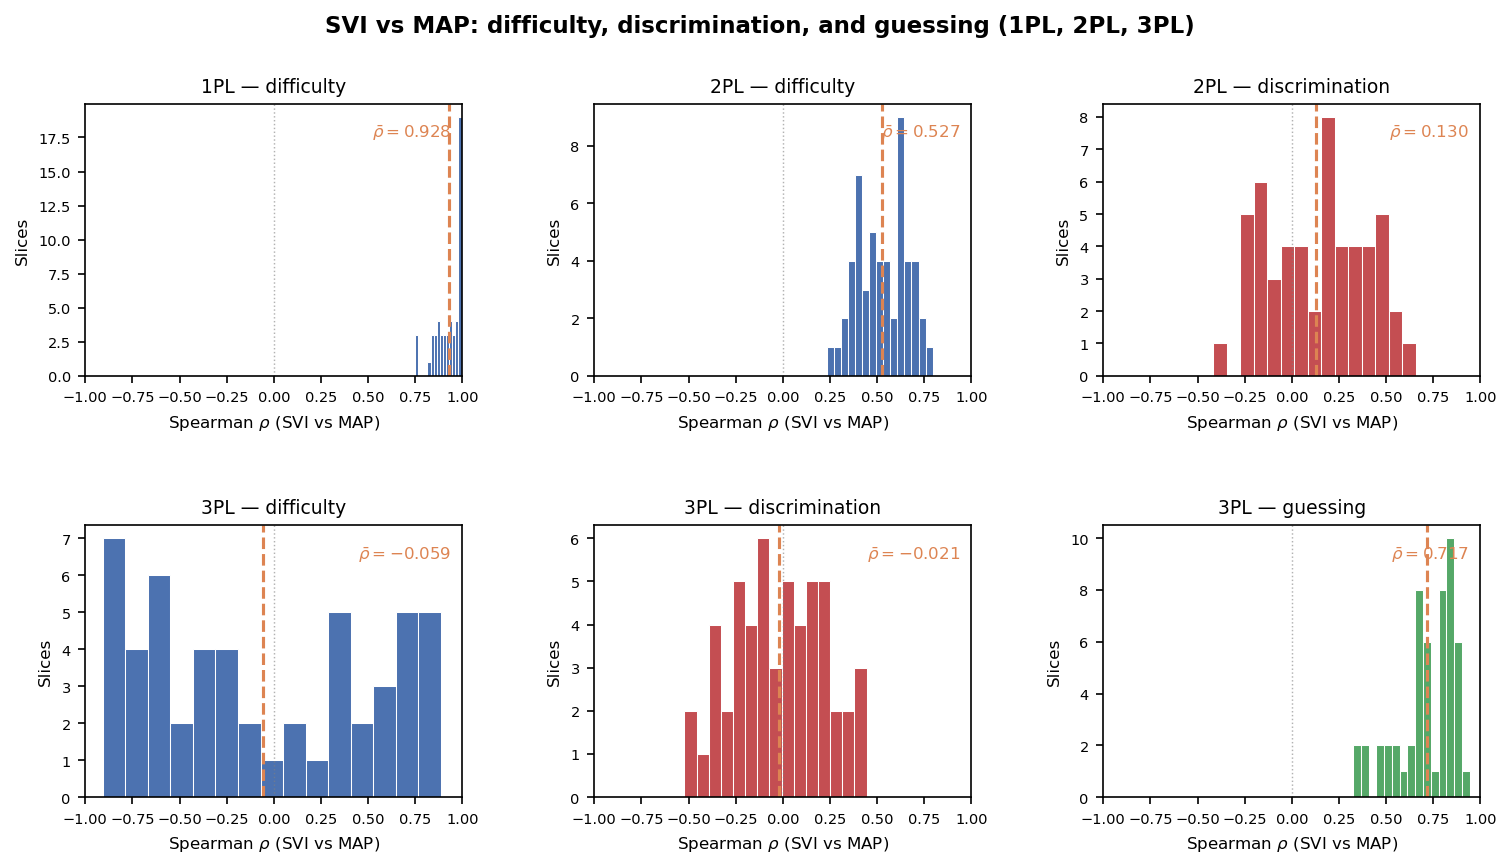
\includegraphics[width=\linewidth]{svi_vs_map_all}
  \caption{Per-slice Spearman $\rho$ between SVI and MAP estimates for each
    (model, parameter) combination across all 53 benchmark slices. Dashed
    orange lines mark the mean $\rho$ per panel. 1PL difficulty shows strong
    SVI--MAP agreement; discrimination collapses under SVI for 2PL and 3PL.}
  \label{fig:svi_vs_map_all}
\end{figure}


To verify that our choice of inference method does not confound cross-model
comparisons, we fit a MAP-based 1PL to all 53 benchmark slices alongside
MAP-based 2PL and 3PL, and compare difficulty, discrimination, and guessing
estimates against their SVI counterparts (\autoref{fig:svi_vs_map_all}).

For \textbf{1PL}, SVI and MAP difficulty estimates are highly concordant
(mean $\rho = 0.928$, min $= 0.749$, max $= 0.996$), confirming that using
\texttt{py-irt}'s SVI for 1PL does not affect our results.

For \textbf{2PL and 3PL}, the comparison directly illustrates why MAP is
necessary. Discrimination estimates are near-uncorrelated across the two
methods (2PL: mean $\rho = 0.130$; 3PL: mean $\rho = -0.021$): SVI drives
discrimination toward zero (2PL) or negative values (3PL), while MAP with
softplus-constrained discrimination recovers psychometrically meaningful
positive values. Under 3PL the distortion is severe enough to corrupt even
difficulty estimates (mean $\rho = -0.059$). The guessing parameter is
relatively robust across inference methods (mean $\rho = 0.717$), consistent
with its role as a lower-asymptote constraint less sensitive to discrimination
interactions.

\section{Spearman Rank Correlation Heatmaps}
\label{app:heatmaps}

In main text, \autoref{fig:spearman_heatmaps} shows pairwise Spearman
rank correlations for item \emph{difficulty} while \autoref{fig:spearman_disc_lambda}
provides the corresponding heatmaps for \emph{discrimination} ($a$,
available from 2PL onward) and \emph{guessing} ($c$, 3PL only). Here, we provide a more detailed discussion of findings:

\paragraph{Discrimination ($a$).}Discrimination parameters show low cross-lingual agreement under both 2PL and 3PL. For MGSM 2PL, the mean pairwise $\rho = 0.103$
(range $[-0.068$ (English--Japanese) to $0.275$ (German--Russian)]):
while the estimates are positive and psychometrically meaningful within each language,
they do not agree strongly across languages, indicating that how sharply an item
discriminates between models is a language-specific property of item formulation.
Under MGSM 3PL the mean pairwise $\rho = 0.098$ (range $[-0.085,\, 0.241]$),
consistent with the additional guessing parameter absorbing some residual shared
signal and leaving discrimination with little cross-lingual structure.
MMLU 2PL and 3PL show a similarly low average discrimination agreement
($\bar{\rho} \approx 0.10$ for both), indicating that even with larger per-domain
item pools, discrimination does not generalize cross-lingually.
This provides clear evidence that discrimination captures language-idiosyncratic
surface features of item formulation rather than a shared psychometric property.

\paragraph{Guessing ($c$).}
The guessing parameter tells a markedly different story.
For MGSM 3PL, $\bar{\rho} = 0.344$ (range $[0.109,\, 0.584]$), with
Bengali--English achieving the strongest agreement ($\rho = 0.584$),
a plausible finding if both language versions impose similar chance-level
accessibility on the same underlying items.
Russian--Thai is the weakest pair ($\rho = 0.109$); all pairs remain positive.
For MMLU 3PL, guessing agreement is even stronger:
$\bar{\rho} = 0.554$ (range $[0.239,\, 0.756]$), with every language
pair yielding a positive correlation and Spanish--French the most
consistent ($\rho = 0.756$).
The consistently positive guessing correlations, in contrast to near-zero
or negative discrimination correlations under the same model, suggest that
lower-bound response behavior is a genuine language-invariant property: some items simply impose a floor on the probability of a correct
response regardless of the language of presentation, while discrimination
is driven by language-specific surface features of the item formulation.

\paragraph{Science vs Non-Science Domain}
Figure~\ref{fig:science_vs_nonscience} shows the 2$\times$3 grid of averaged
Spearman difficulty heatmaps for science vs non-science domains across the three
IRT model variants.
Under 1PL, science heatmaps show a predominantly warm palette
(Kendall's $W = 0.647$, $\bar{\rho} = 0.588$), while non-science is already
lower ($\bar{\rho} = 0.492$, $W = 0.564$).
Under MAP-fitted 2PL and 3PL, the science advantage is maintained: science
domains achieve $\bar{\rho} = 0.559$, $W = 0.620$ (2PL) and $\bar{\rho} = 0.581$,
$W = 0.640$ (3PL), while non-science remains somewhat lower at $\bar{\rho} = 0.420$,
$W = 0.501$ (2PL) and $\bar{\rho} = 0.479$, $W = 0.553$ (3PL).
Both domain types maintain moderate cross-lingual concordance across all model
variants, with science items consistently showing stronger agreement.
This reflects that science items test well-defined reasoning steps or unambiguous
facts whose difficulty is partly preserved under translation, whereas non-science
difficulty is dominated by culturally situated knowledge and nuanced phrasing
that shifts substantially across languages.

\begin{figure*}[!t]
  \centering
  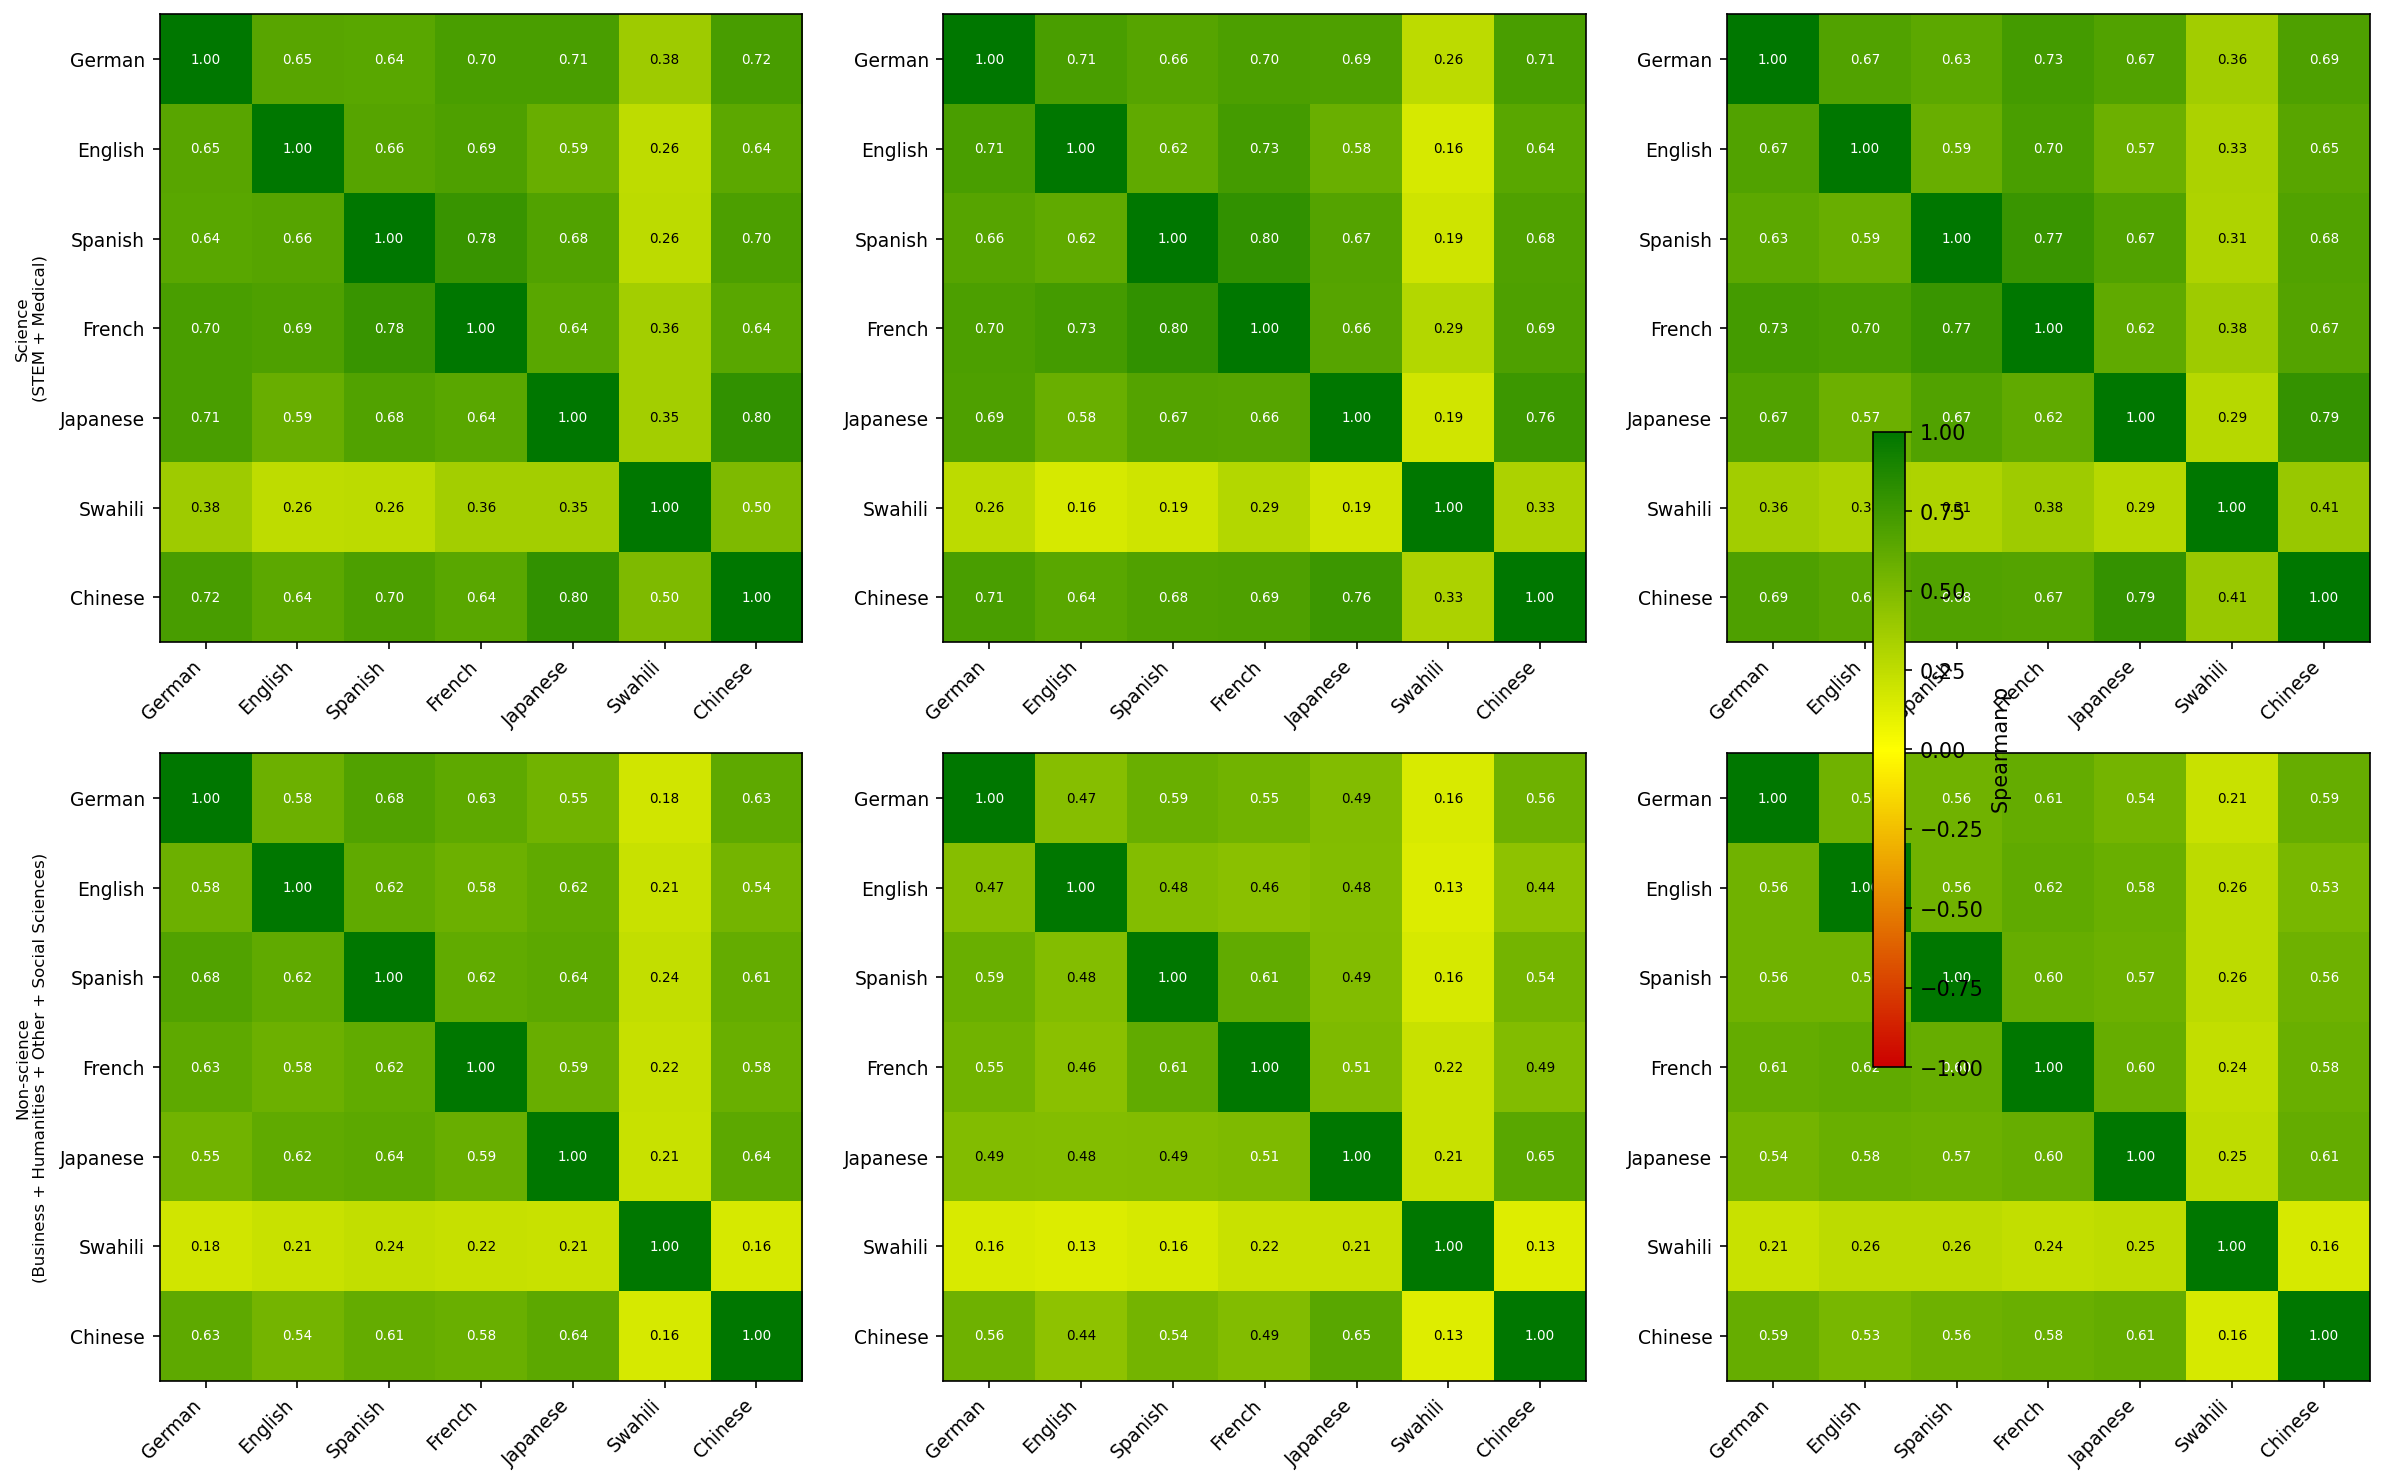
\includegraphics[width=\linewidth]{mmlu_science_vs_nonscience}
  \caption{Pairwise Spearman rank correlation of item \emph{difficulty} across
    languages for MMLU, split by domain type (rows) and IRT model variant (columns).
    \textbf{Top row:} Science domains (STEM + Medical), averaged element-wise.
    \textbf{Bottom row:} Non-science domains (Business + Humanities + Other +
    Social Sciences), averaged element-wise.
    Colour encodes $\rho \in [-1,+1]$: red $= -1$, yellow $= 0$, green $= +1$.}
  \label{fig:science_vs_nonscience}
\end{figure*}

\section{Per-Item Rank Stability Distributions}
\label{app:rank_stability}

\autoref{fig:gsm_item_rank_stability} and \autoref{fig:mmlu_item_rank_stability} shows per-item rank standard deviation sorted ascending (most to
least consistent left to right). Each bar is one item; bar height is the
standard deviation of its rank position across all languages.
Multi-parameter models show one sub-panel per parameter.

\begin{figure*}[!t]
  \centering
  \begin{subfigure}[t]{0.32\linewidth}
    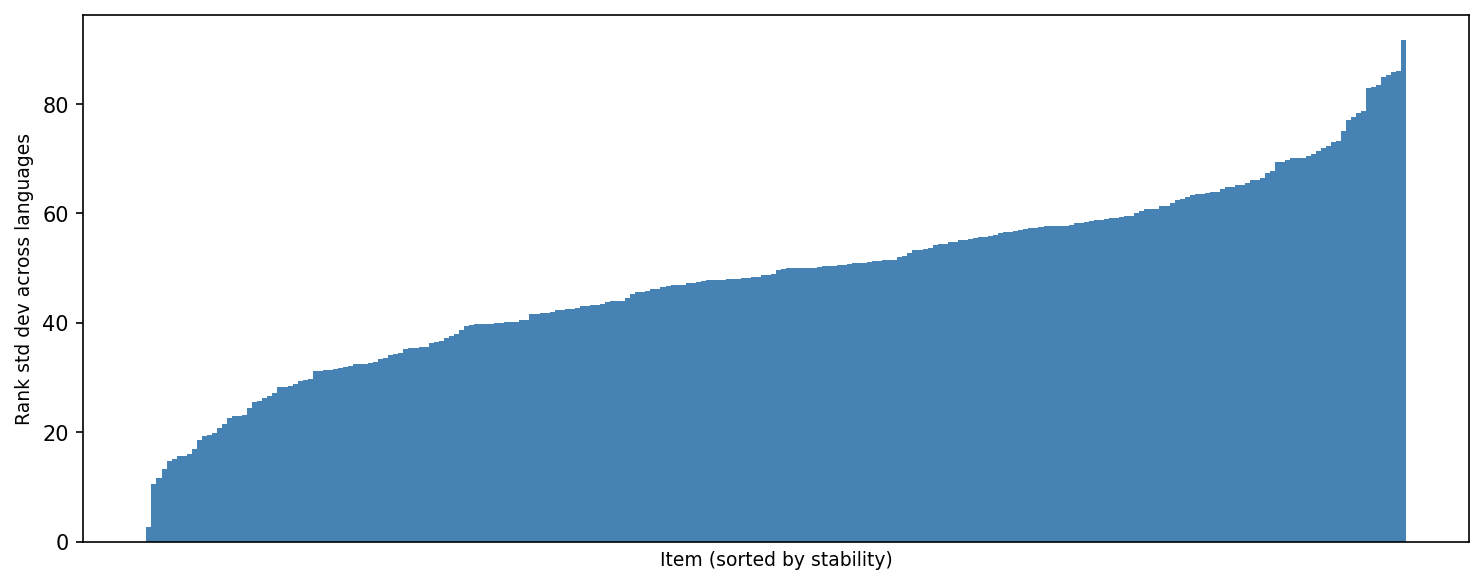
\includegraphics[width=\linewidth]{gsm_1pl_item_rank_stability}
    \caption{1PL (difficulty)}\label{fig:gsm_1pl_stab}
  \end{subfigure}\hfill
  \begin{subfigure}[t]{0.32\linewidth}
    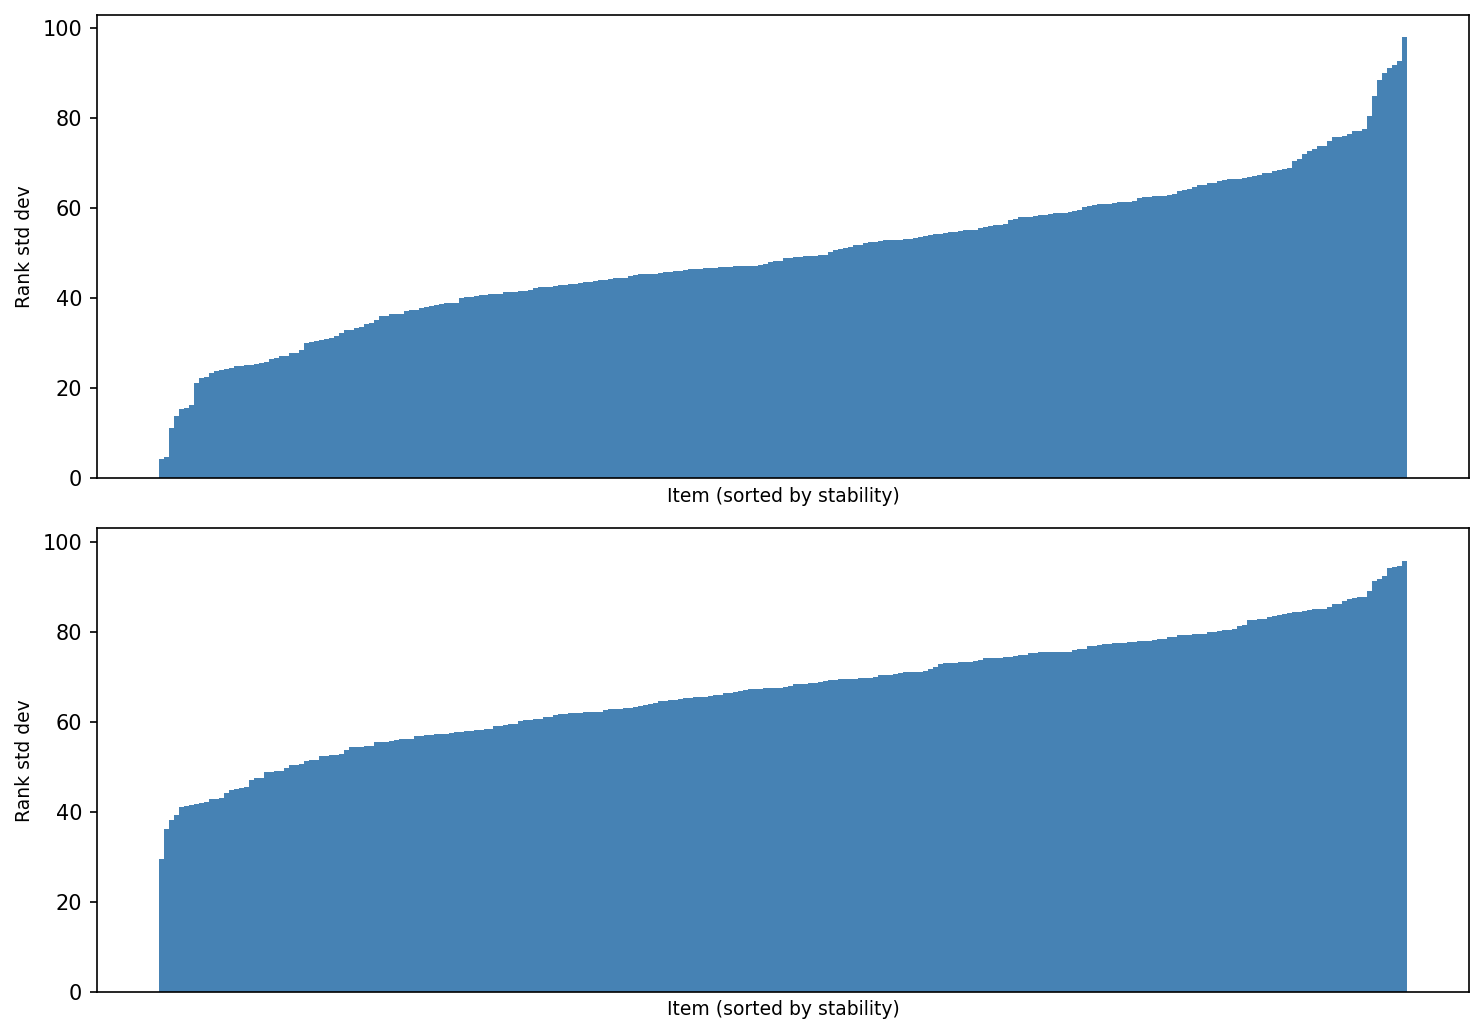
\includegraphics[width=\linewidth]{gsm_2pl_item_rank_stability}
    \caption{2PL (difficulty + discrimination)}\label{fig:gsm_2pl_stab}
  \end{subfigure}\hfill
  \begin{subfigure}[t]{0.32\linewidth}
    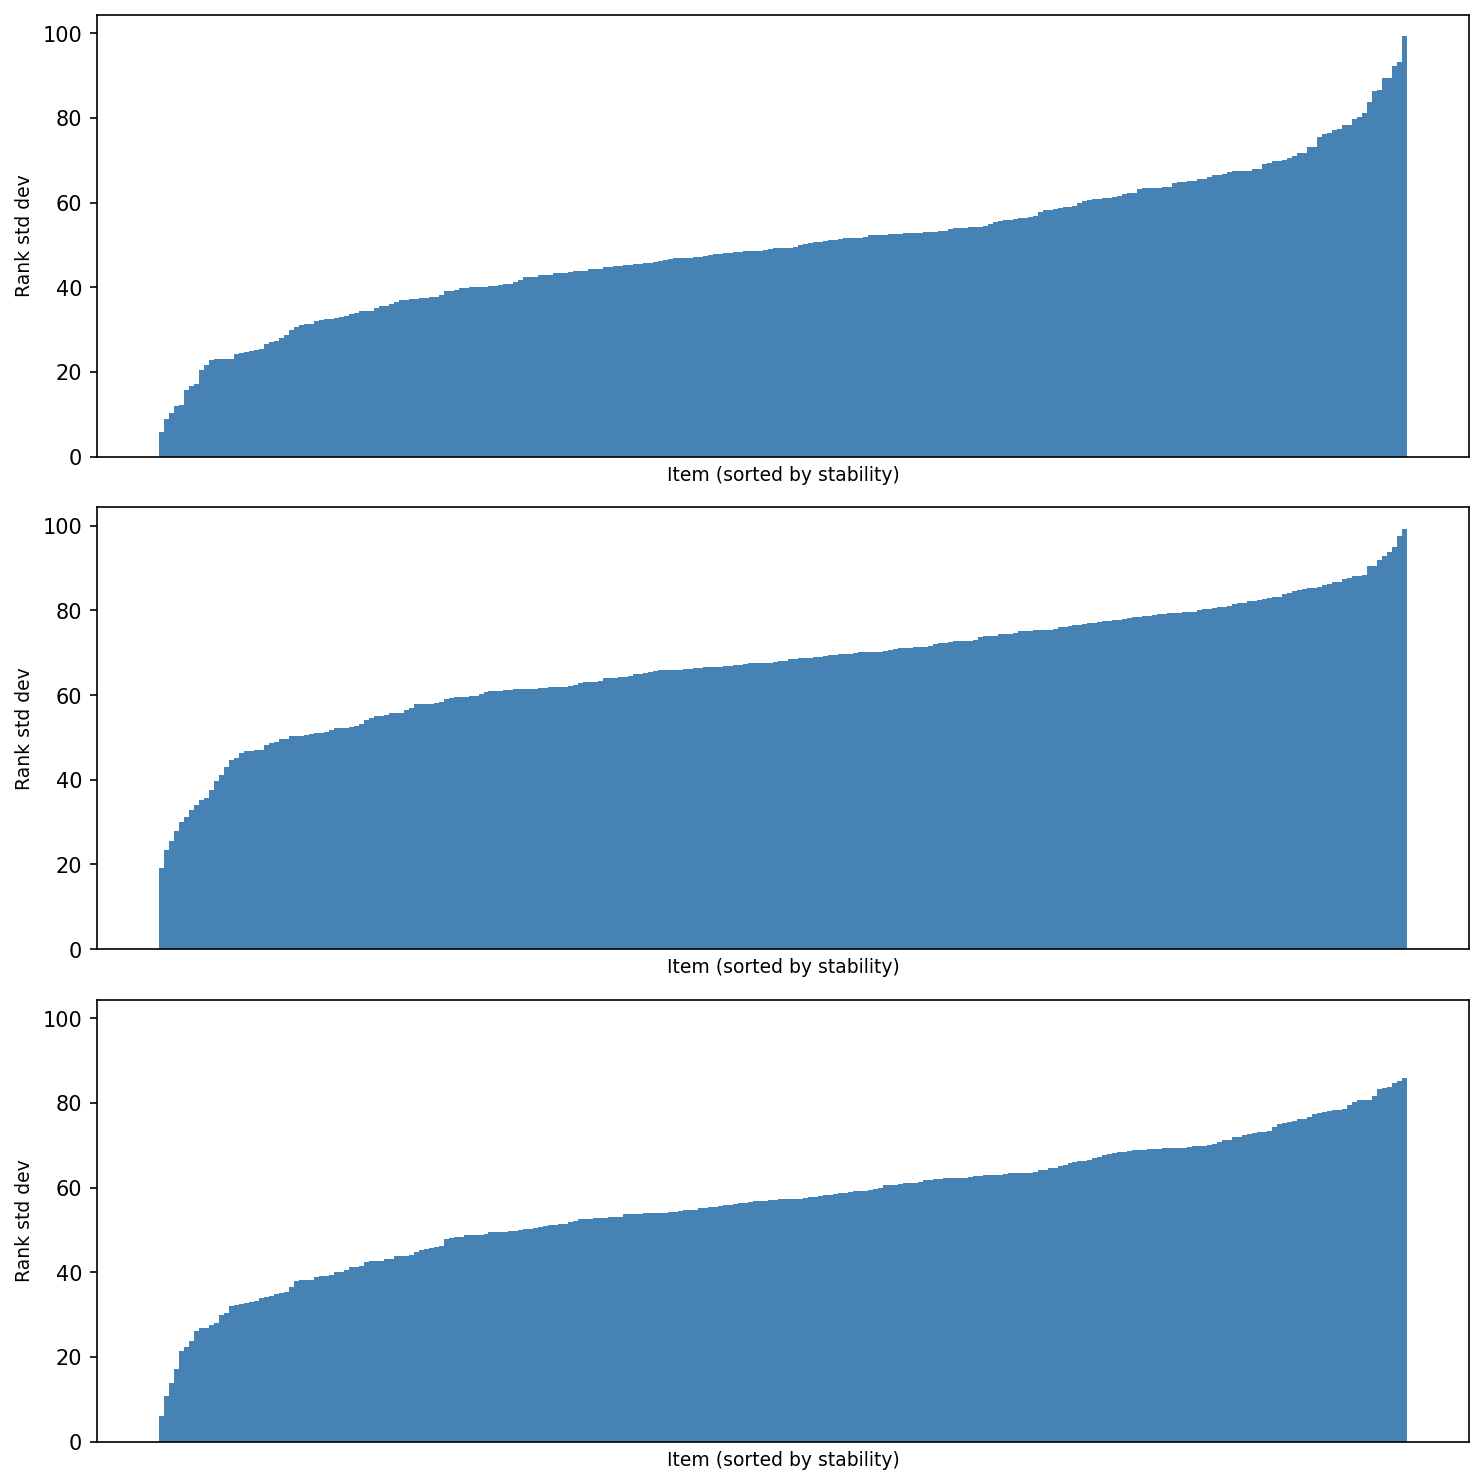
\includegraphics[width=\linewidth]{gsm_3pl_item_rank_stability}
    \caption{3PL (difficulty + discrimination + guessing)}\label{fig:gsm_3pl_stab}
  \end{subfigure}
  \caption{MGSM per-item rank standard deviation across 11 languages (250 items). Each subfigure shows all parameters for that model variant stacked vertically.}
  \label{fig:gsm_item_rank_stability}
\end{figure*}

\begin{figure*}[!t]
  \centering
  \begin{subfigure}[t]{0.32\linewidth}
    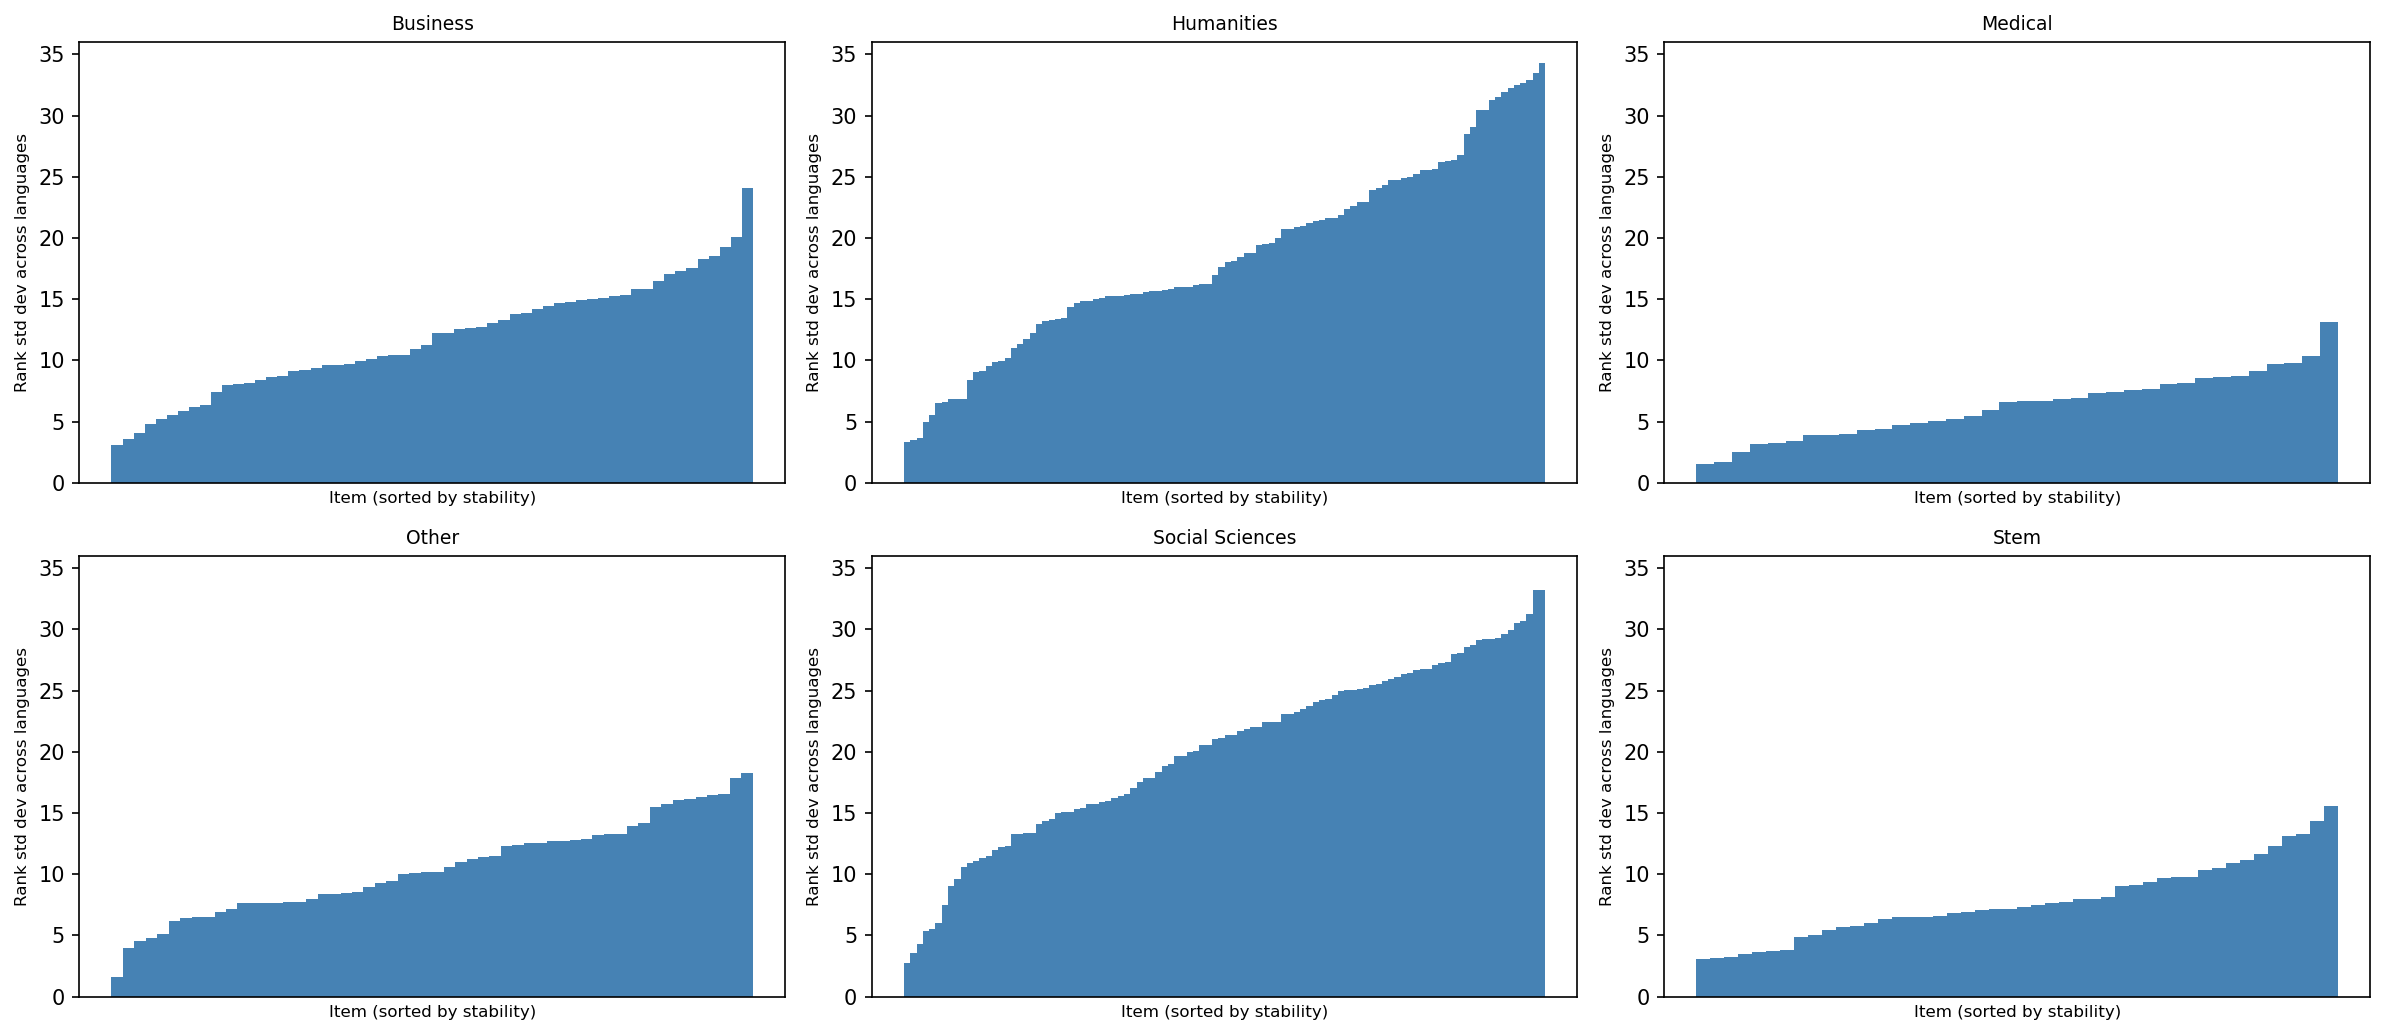
\includegraphics[width=\linewidth]{mmlu_1pl_item_rank_stability}
    \caption{1PL (difficulty)}\label{fig:mmlu_1pl_stab}
  \end{subfigure}\hfill
  \begin{subfigure}[t]{0.32\linewidth}
    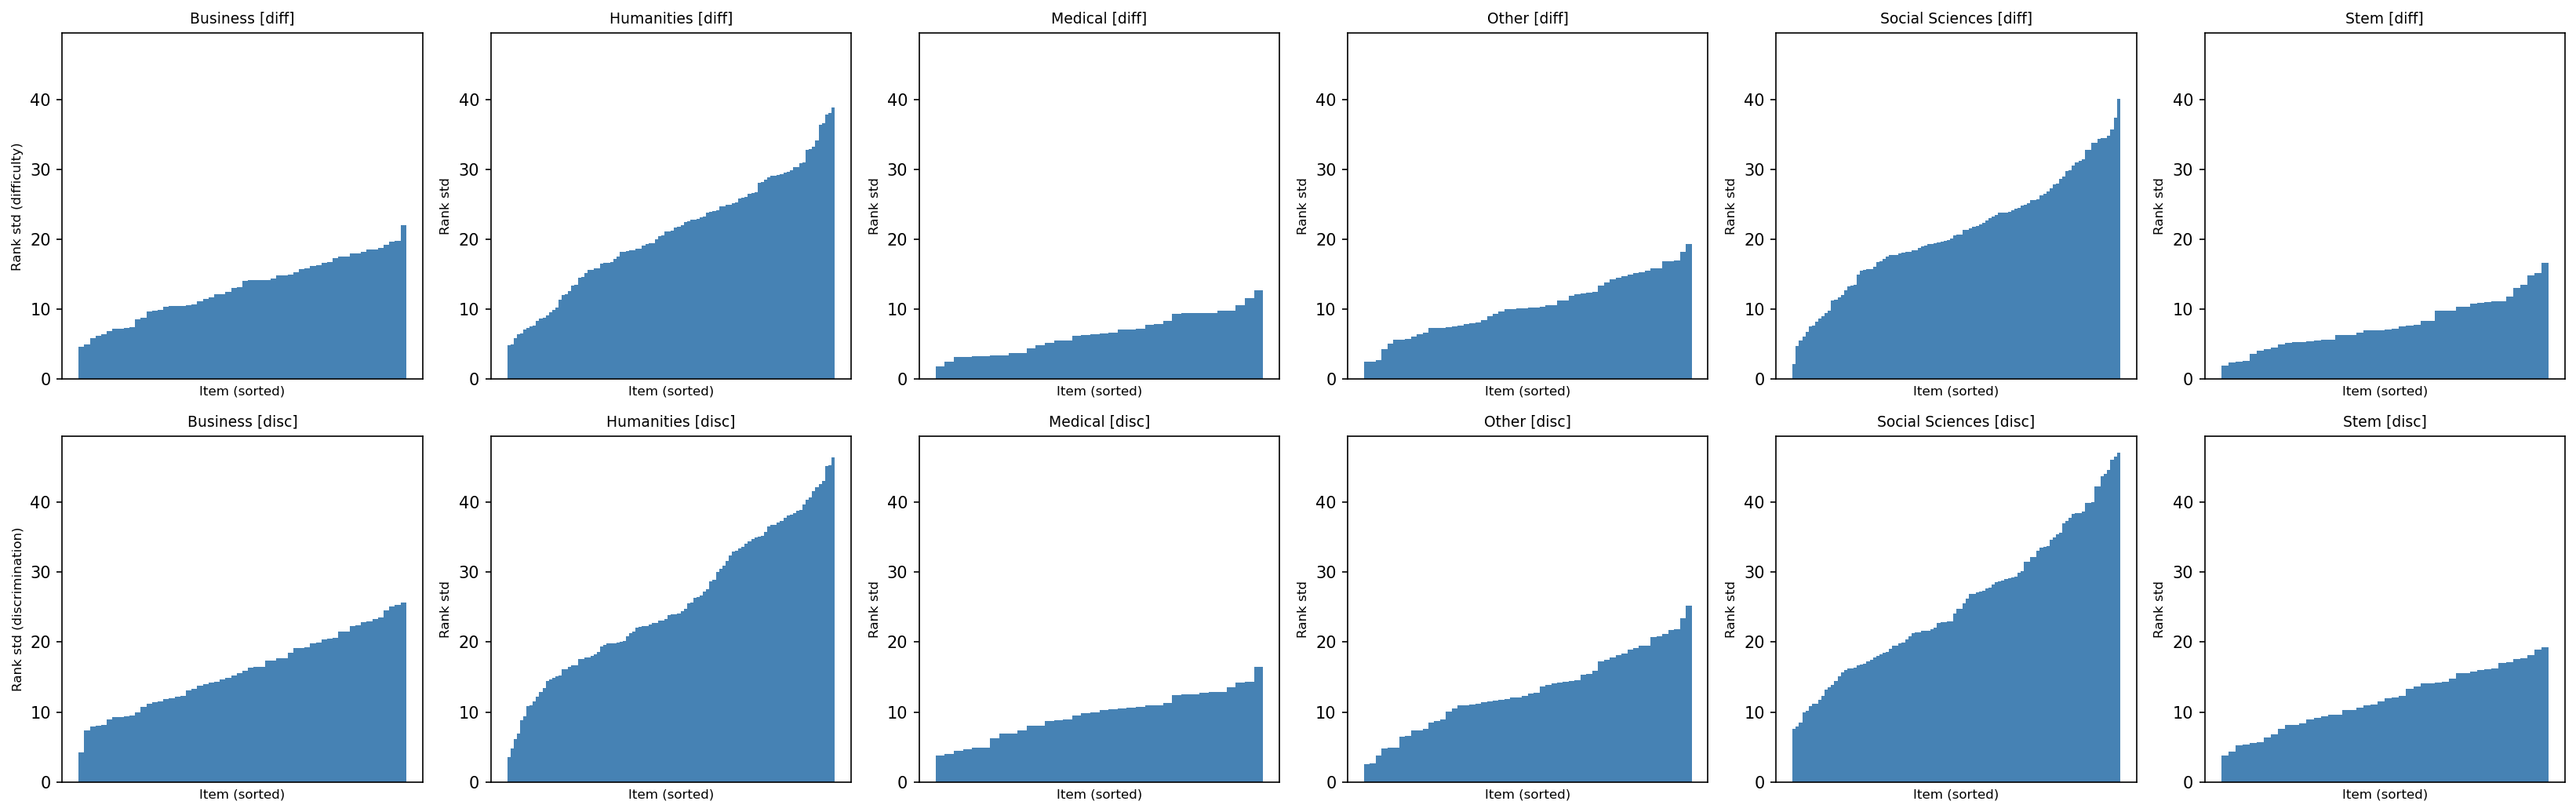
\includegraphics[width=\linewidth]{mmlu_2pl_item_rank_stability}
    \caption{2PL (difficulty + discrimination)}\label{fig:mmlu_2pl_stab}
  \end{subfigure}\hfill
  \begin{subfigure}[t]{0.32\linewidth}
    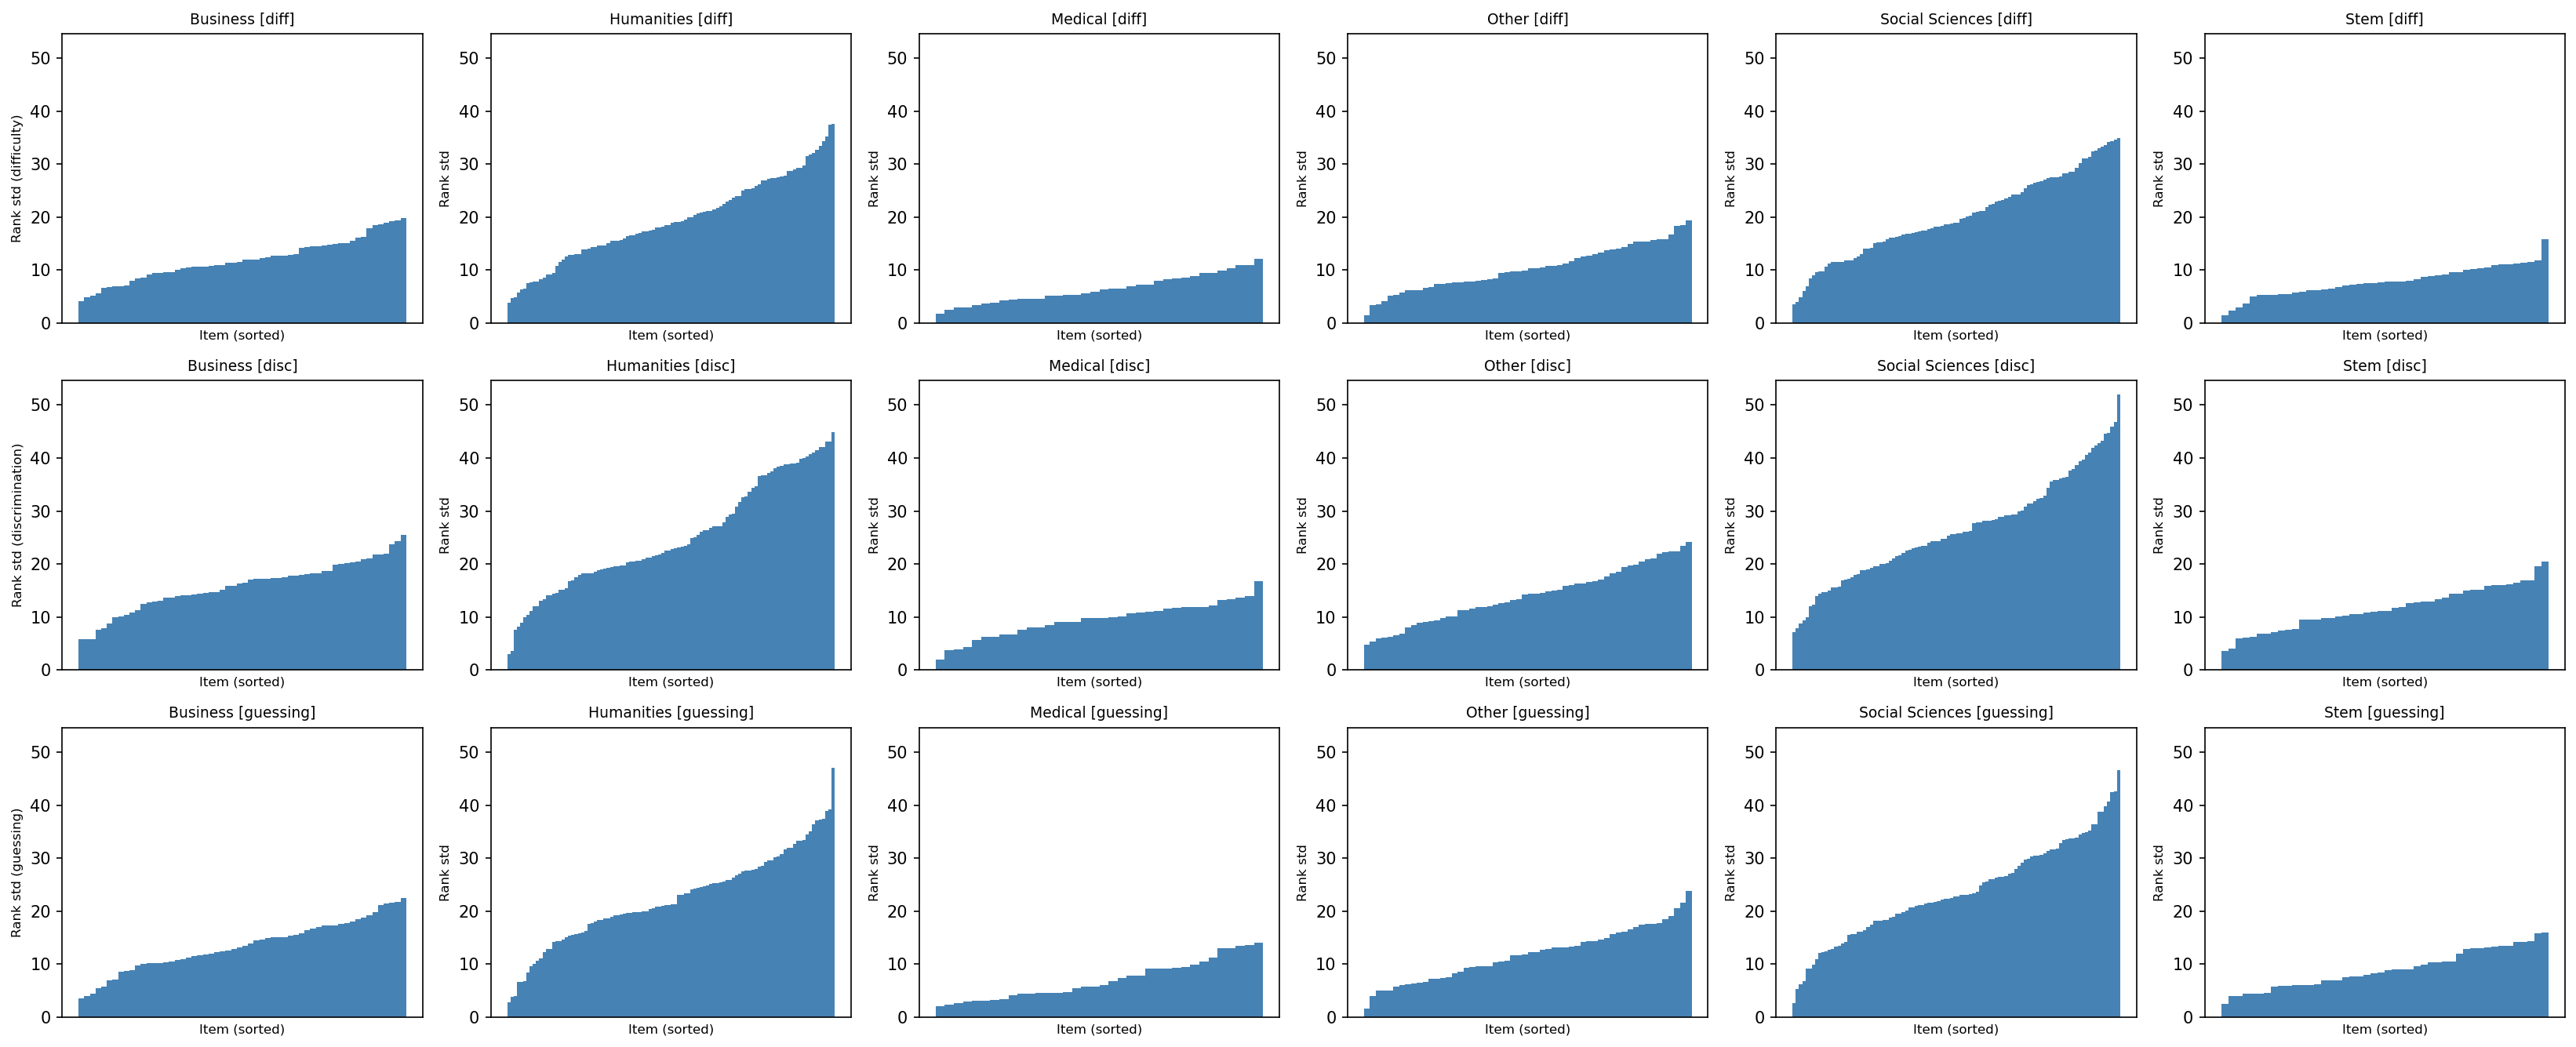
\includegraphics[width=\linewidth]{mmlu_3pl_item_rank_stability}
    \caption{3PL (difficulty + discrimination + guessing)}\label{fig:mmlu_3pl_stab}
  \end{subfigure}
  \caption{MMLU per-item rank standard deviation across 7 languages, pooled
    over six domains ($n \leq 102$ items per domain).}
  \label{fig:mmlu_item_rank_stability}
\end{figure*}

\section{Within-Language Model Fit}
\label{app:withinlangfits}

To assess within-language fit quality for each IRT variant, we report
the MAP negative log-likelihood per observation ($-\ell/\text{obs}$) at convergence,
where lower values indicate better fit.
\autoref{tab:elbo_per_slice} reports these values for every slice.
As expected under correct model fitting (2PL nests 1PL; 3PL nests 2PL),
2PL achieves better fit than 1PL on all 53 slices, and 3PL achieves better fit than 2PL on all 53 slices.
The improvement is larger on MMLU (mean 1PL $-\ell/\text{obs} = 0.180$ vs 2PL $0.127$ vs 3PL $0.124$)
than on MGSM (mean 1PL $0.426$ vs 2PL $0.389$ vs 3PL $0.389$),
consistent with MMLU's more heterogeneous item difficulty permitting greater discrimination by 2PL,
and the guessing parameter capturing floor-level response probabilities in knowledge-intensive domains.

\begin{table*}[t]
  \centering
  \small
  \begin{tabular}{llccc}
    \toprule
    \textbf{Benchmark} & \textbf{Slice} & \textbf{1PL} & \textbf{2PL} & \textbf{3PL} \\
    \midrule
    MGSM & \texttt{bn} & 0.360 & 0.311 & 0.313 \\
         & \texttt{de} & 0.453 & 0.416 & 0.415 \\
         & \texttt{en} & 0.420 & 0.383 & 0.381 \\
         & \texttt{es} & 0.492 & 0.464 & 0.463 \\
         & \texttt{fr} & 0.454 & 0.420 & 0.420 \\
         & \texttt{ja} & 0.466 & 0.436 & 0.435 \\
         & \texttt{ru} & 0.479 & 0.445 & 0.442 \\
         & \texttt{sw} & 0.405 & 0.366 & 0.367 \\
         & \texttt{te} & 0.284 & 0.236 & 0.244 \\
         & \texttt{th} & 0.445 & 0.412 & 0.412 \\
         & \texttt{zh} & 0.427 & 0.391 & 0.391 \\
    \midrule
    MMLU  & \texttt{de}\_business        & 0.176 & 0.137 & 0.138 \\
          & \texttt{de}\_humanities      & 0.139 & 0.104 & 0.104 \\
          & \texttt{de}\_medical         & 0.122 & 0.077 & 0.077 \\
          & \texttt{de}\_other           & 0.150 & 0.102 & 0.101 \\
          & \texttt{de}\_social\_sciences & 0.166 & 0.132 & 0.129 \\
          & \texttt{de}\_stem            & 0.222 & 0.151 & 0.146 \\
          & \texttt{en}\_business        & 0.108 & 0.066 & 0.062 \\
          & \texttt{en}\_humanities      & 0.112 & 0.078 & 0.081 \\
          & \texttt{en}\_medical         & 0.113 & 0.092 & 0.095 \\
          & \texttt{en}\_other           & 0.155 & 0.122 & 0.119 \\
          & \texttt{en}\_social\_sciences & 0.151 & 0.113 & 0.112 \\
          & \texttt{en}\_stem            & 0.178 & 0.125 & 0.122 \\
          & \texttt{es}\_business        & 0.163 & 0.124 & 0.119 \\
          & \texttt{es}\_humanities      & 0.126 & 0.085 & 0.088 \\
          & \texttt{es}\_medical         & 0.153 & 0.088 & 0.078 \\
          & \texttt{es}\_other           & 0.186 & 0.137 & 0.133 \\
          & \texttt{es}\_social\_sciences & 0.137 & 0.109 & 0.106 \\
          & \texttt{es}\_stem            & 0.213 & 0.151 & 0.145 \\
          & \texttt{fr}\_business        & 0.174 & 0.134 & 0.135 \\
          & \texttt{fr}\_humanities      & 0.123 & 0.093 & 0.093 \\
          & \texttt{fr}\_medical         & 0.141 & 0.091 & 0.095 \\
          & \texttt{fr}\_other           & 0.175 & 0.124 & 0.117 \\
          & \texttt{fr}\_social\_sciences & 0.146 & 0.113 & 0.111 \\
          & \texttt{fr}\_stem            & 0.231 & 0.170 & 0.165 \\
          & \texttt{ja}\_business        & 0.162 & 0.086 & 0.077 \\
          & \texttt{ja}\_humanities      & 0.140 & 0.095 & 0.093 \\
          & \texttt{ja}\_medical         & 0.158 & 0.086 & 0.083 \\
          & \texttt{ja}\_other           & 0.182 & 0.128 & 0.120 \\
          & \texttt{ja}\_social\_sciences & 0.184 & 0.137 & 0.134 \\
          & \texttt{ja}\_stem            & 0.201 & 0.121 & 0.114 \\
          & \texttt{sw}\_business        & 0.332 & 0.260 & 0.255 \\
          & \texttt{sw}\_humanities      & 0.319 & 0.246 & 0.241 \\
          & \texttt{sw}\_medical         & 0.251 & 0.161 & 0.155 \\
          & \texttt{sw}\_other           & 0.294 & 0.233 & 0.231 \\
          & \texttt{sw}\_social\_sciences & 0.337 & 0.258 & 0.251 \\
          & \texttt{sw}\_stem            & 0.305 & 0.224 & 0.219 \\
          & \texttt{zh}\_business        & 0.137 & 0.079 & 0.078 \\
          & \texttt{zh}\_humanities      & 0.136 & 0.095 & 0.090 \\
          & \texttt{zh}\_medical         & 0.125 & 0.077 & 0.071 \\
          & \texttt{zh}\_other           & 0.198 & 0.132 & 0.123 \\
          & \texttt{zh}\_social\_sciences & 0.140 & 0.105 & 0.103 \\
          & \texttt{zh}\_stem            & 0.178 & 0.113 & 0.109 \\
    \bottomrule
  \end{tabular}
  \caption{MAP negative log-likelihood per observation ($-\ell/\text{obs}$) for each
    IRT model variant and benchmark slice. Lower values indicate better within-language fit.
    2PL achieves better fit than 1PL, and 3PL achieves better fit than 2PL, on all 53 slices,
    consistent with correct model identification under MAP.}
  \label{tab:elbo_per_slice}
\end{table*}

\section{IIF Theta Sensitivity}
\label{app:theta}

The main analysis evaluates IIF at $\theta = 0$ (median ability). To assess
sensitivity to this choice, we recompute item selections at $\theta \in \{-1,
0, +1\}$ and measure the Jaccard similarity of the resulting top-50\% subsets
across theta values within each model, and cross-model Jaccard at each theta.

\paragraph{Within-model sensitivity.}
Under MAP, 2PL item selection shows meaningful theta sensitivity on both benchmarks:
MGSM 2PL mean $J = 0.639$ between $\theta=-1$ and $\theta=0$; $J = 0.429$ between
$\theta=0$ and $\theta=+1$; $J = 0.232$ between $\theta=-1$ and $\theta=+1$.
This reflects that properly-identified discrimination parameters vary across items,
so IIF rankings depend on theta. 3PL shows similar sensitivity (MGSM: $J = 0.617$,
$0.400$, $0.208$ for the same pairs).
1PL shows moderate theta sensitivity on MGSM (mean $J = 0.727$ between
$\theta=-1$ and $\theta=0$; $J = 0.835$ between $\theta=0$ and $\theta=+1$)
but near-invariance on MMLU (mean $J \geq 0.929$). The greater sensitivity on
MGSM reflects the wider difficulty range of arithmetic items relative to the
narrower MMLU domain slices.

\paragraph{Cross-model concordance across theta.}
\autoref{tab:theta_sensitivity} shows median Jaccard for each model pair at
each $\theta$. The qualitative ordering is preserved across all theta values:
1PL--2PL and 1PL--3PL agreement both remain above the random baseline ($J \approx 0.33$)
at every $\theta$, and 2PL--3PL agreement is consistently high ($J \geq 0.87$).
The conclusion that 2PL and 3PL select overlapping but not identical subsets
relative to 1PL therefore holds across all evaluated ability levels.

\begin{table}[h]
  \centering
  \small
  \begin{tabular}{llcc}
    \toprule
    \textbf{Pair} & $\theta$ & \textbf{MGSM} & \textbf{MMLU} \\
                  &          & median $J$    & median $J$ \\
    \midrule
    1PL vs 2PL & $-1$ & 0.553 & 0.268 \\
               &  $0$ & 0.404 & 0.528 \\
               & $+1$ & 0.506 & 0.672 \\
    \midrule
    1PL vs 3PL & $-1$ & 0.524 & 0.273 \\
               &  $0$ & 0.412 & 0.454 \\
               & $+1$ & 0.543 & 0.672 \\
    \midrule
    2PL vs 3PL & $-1$ & 0.923 & 0.688 \\
               &  $0$ & 0.923 & 0.590 \\
               & $+1$ & 0.866 & 0.895 \\
    \bottomrule
  \end{tabular}
  \caption{Median Jaccard similarity of top-50\% IIF-selected subsets across
    model pairs, evaluated at three theta values. The random-selection baseline
    is $J \approx 0.33$. Qualitative orderings are stable across all theta values.}
  \label{tab:theta_sensitivity}
\end{table}

\section{Compression Ratio Sensitivity}
\label{app:compression}

The main analysis uses a top-50\% IIF cutoff. To assess sensitivity to this
choice, \autoref{tab:compression} reports in-sample median Spearman $\rho$
(subset vs.\ full benchmark) at top-30\%, top-50\%, and top-70\% for each
IRT variant and benchmark.

The qualitative ordering is preserved across all ratios. 1PL is reliable at
50\% and above on both benchmarks; at 30\%, fidelity dips slightly (MMLU mean $\rho = 0.931$).
2PL is competitive on MGSM at all compression levels (mean $\rho \geq 0.939$), but shows
substantially lower fidelity on MMLU at all thresholds (mean $\rho = 0.771$--$0.875$),
remaining below 1PL. 3PL follows a similar pattern, with MMLU fidelity
lower than 2PL and 1PL at all ratios (mean $\rho = 0.674$--$0.721$).
The 50\% default is the point where 1PL clears the random baseline
reliably across all slices while achieving meaningful compression.

\begin{table}[h]
  \centering
  \small
  \begin{tabular}{llcc}
    \toprule
    \textbf{Model} & \textbf{Top-$k$} & \textbf{MGSM} & \textbf{MMLU} \\
                   &                  & median $\rho$ & median $\rho$ \\
    \midrule
    1PL & 30\% & 0.939 & 0.931 \\
        & 50\% & 0.977 & 0.983 \\
        & 70\% & 0.994 & 0.999 \\
    \midrule
    2PL & 30\% & 0.939 & 0.771 \\
        & 50\% & 0.963 & 0.844 \\
        & 70\% & 0.974 & 0.875 \\
    \midrule
    3PL & 30\% & 0.939 & 0.674 \\
        & 50\% & 0.961 & 0.721 \\
        & 70\% & 0.975 & 0.717 \\
    \bottomrule
  \end{tabular}
  \caption{In-sample ranking fidelity (median Spearman $\rho$, subset
    vs.\ full benchmark) at three compression ratios. The random-selection
    baseline is $\rho \approx 0.96$ for MGSM and $\approx 0.70$ for MMLU.
    1PL conclusions are stable across all ratios; 2PL and 3PL fail on MMLU
    at every threshold.}
  \label{tab:compression}
\end{table}



\section{Subset Ranking Fidelity}
\label{app:ranking_fidelity}

Here, we provide: per-slice fidelity across all benchmark variants (Figure~\ref{fig:same_lang_boxplot}), and per-model accuracy-prediction scatter for in-sample (Figure~\ref{fig:insample_scatter}) and held-out (Figure~\ref{fig:heldout_scatter}) evaluations.

\paragraph{Per-slice Fidelity (Figure~\ref{fig:same_lang_boxplot}).}
Each dot is one benchmark slice — 11 MGSM language slices and 42 MMLU
language$\times$domain slices.
For MGSM, 1PL is uniformly strong across all 11 languages (median $\rho = 0.982$,
IQR entirely above $\rho = 0.95$), with no language slice falling below the
random baseline. 2PL is similarly strong (median $\rho = 0.971$, IQR $0.957$--$0.976$),
with the minimum at $\rho = 0.915$, well above the random baseline; no slice fails badly.
3PL is comparable (median $\rho = 0.973$, IQR $0.955$--$0.976$, min $0.911$).
For MMLU, the contrast between 1PL and the multi-parameter models sharpens considerably.
1PL achieves median $\rho = 1.000$ — the majority of the 42 slices reach perfect
rank correlation — with all slices well above the random baseline ($\rho \approx 0.70$).
2PL falls to median $\rho = 0.878$ (IQR $0.740$--$0.970$, min $0.354$): most MMLU slices
retain useful fidelity, but the lower tail extends below the random baseline on a minority of
slices.
3PL is further reduced (median $\rho = 0.764$, IQR $0.594$--$0.892$, min $0.290$),
with more slices falling below the reference line than under 2PL.

\begin{figure*}[t]
  \centering
  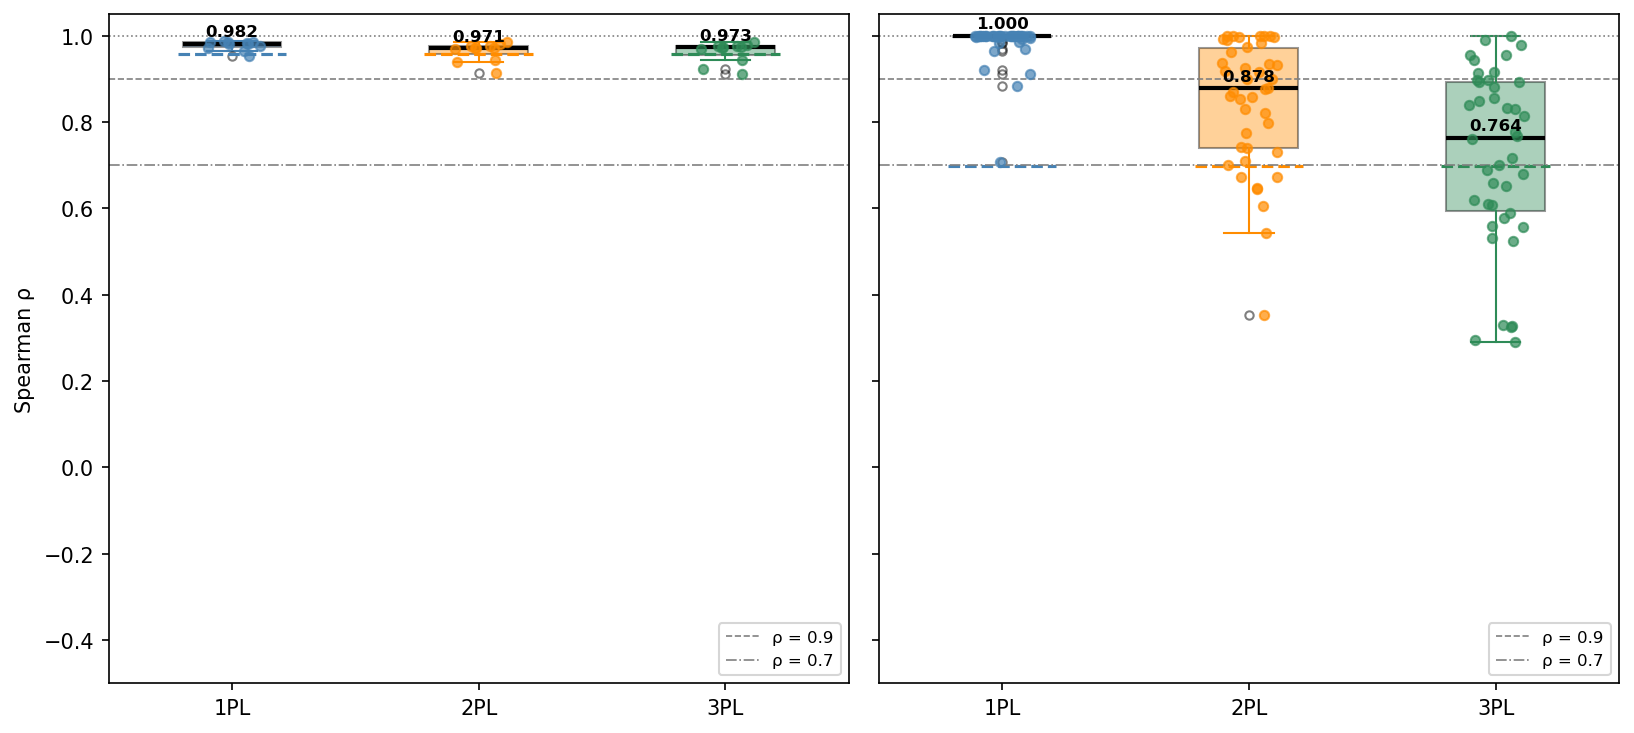
\includegraphics[width=\linewidth]{same_lang_boxplot}
  \caption{Distribution of Spearman $\rho$ (subset vs.\ full benchmark) across all
    in-sample benchmark slices: 11 MGSM language slices (left) and 42 MMLU
    language$\times$domain slices (right).
    Each dot is one slice; annotated values are medians.
    Dashed lines mark $\rho = 0.90$ and $\rho = 0.70$; the dotted line at the
    top marks $\rho = 1.0$.
    The random-item baseline ($\rho \approx 0.96$ for MGSM, $\approx 0.70$ for MMLU)
    is shown as a dashed reference.}
  \label{fig:same_lang_boxplot}
\end{figure*}

\paragraph{In-sample accuracy prediction (Figure~\ref{fig:insample_scatter}).}
Each point is one (model, benchmark-slice) pair ($n = 1{,}122$ for MGSM;
$n = 4{,}320$ for MMLU).
The dashed $y = x$ line marks perfect accuracy prediction; deviations from it
indicate systematic bias in how the subset estimates a model's full-benchmark score.
Under 1PL, MGSM points cluster tightly near the diagonal
(MAE $= 0.086$, bias $= +0.026$): the subset very slightly overestimates
full accuracy, consistent with IIF at $\theta = 0$ selecting items near median
difficulty, which form a marginally easier sub-pool than the benchmark as a whole.
Under 1PL, MMLU shows the opposite bias (MAE $= 0.098$, bias $= -0.065$):
the IIF-selected items are slightly harder than the MMLU average because
IIF peaks for items with difficulty $b \approx 0$, which are harder than
the typical MMLU item (most items are easier than chance for these models).
Consequently, subset accuracy understates full-benchmark accuracy by about
six percentage points on average.
Under 2PL and 3PL, MGSM accuracy prediction is close to 1PL
(MGSM 2PL MAE $= 0.103$, bias $= +0.073$; 3PL MAE $= 0.101$, bias $= +0.079$).
On MMLU, 2PL IIF introduces a moderate positive bias ($+0.080$, MAE $= 0.117$): the
discrimination-weighted selection still over-selects items where models score high,
inflating subset accuracy estimates relative to the full benchmark by about 8 percentage points.
3PL shows a larger positive bias on MMLU (bias $= +0.177$, MAE $= 0.183$), reflecting
that the guessing parameter further amplifies the selection of items with high response
probabilities.

\begin{figure*}[t]
  \centering
  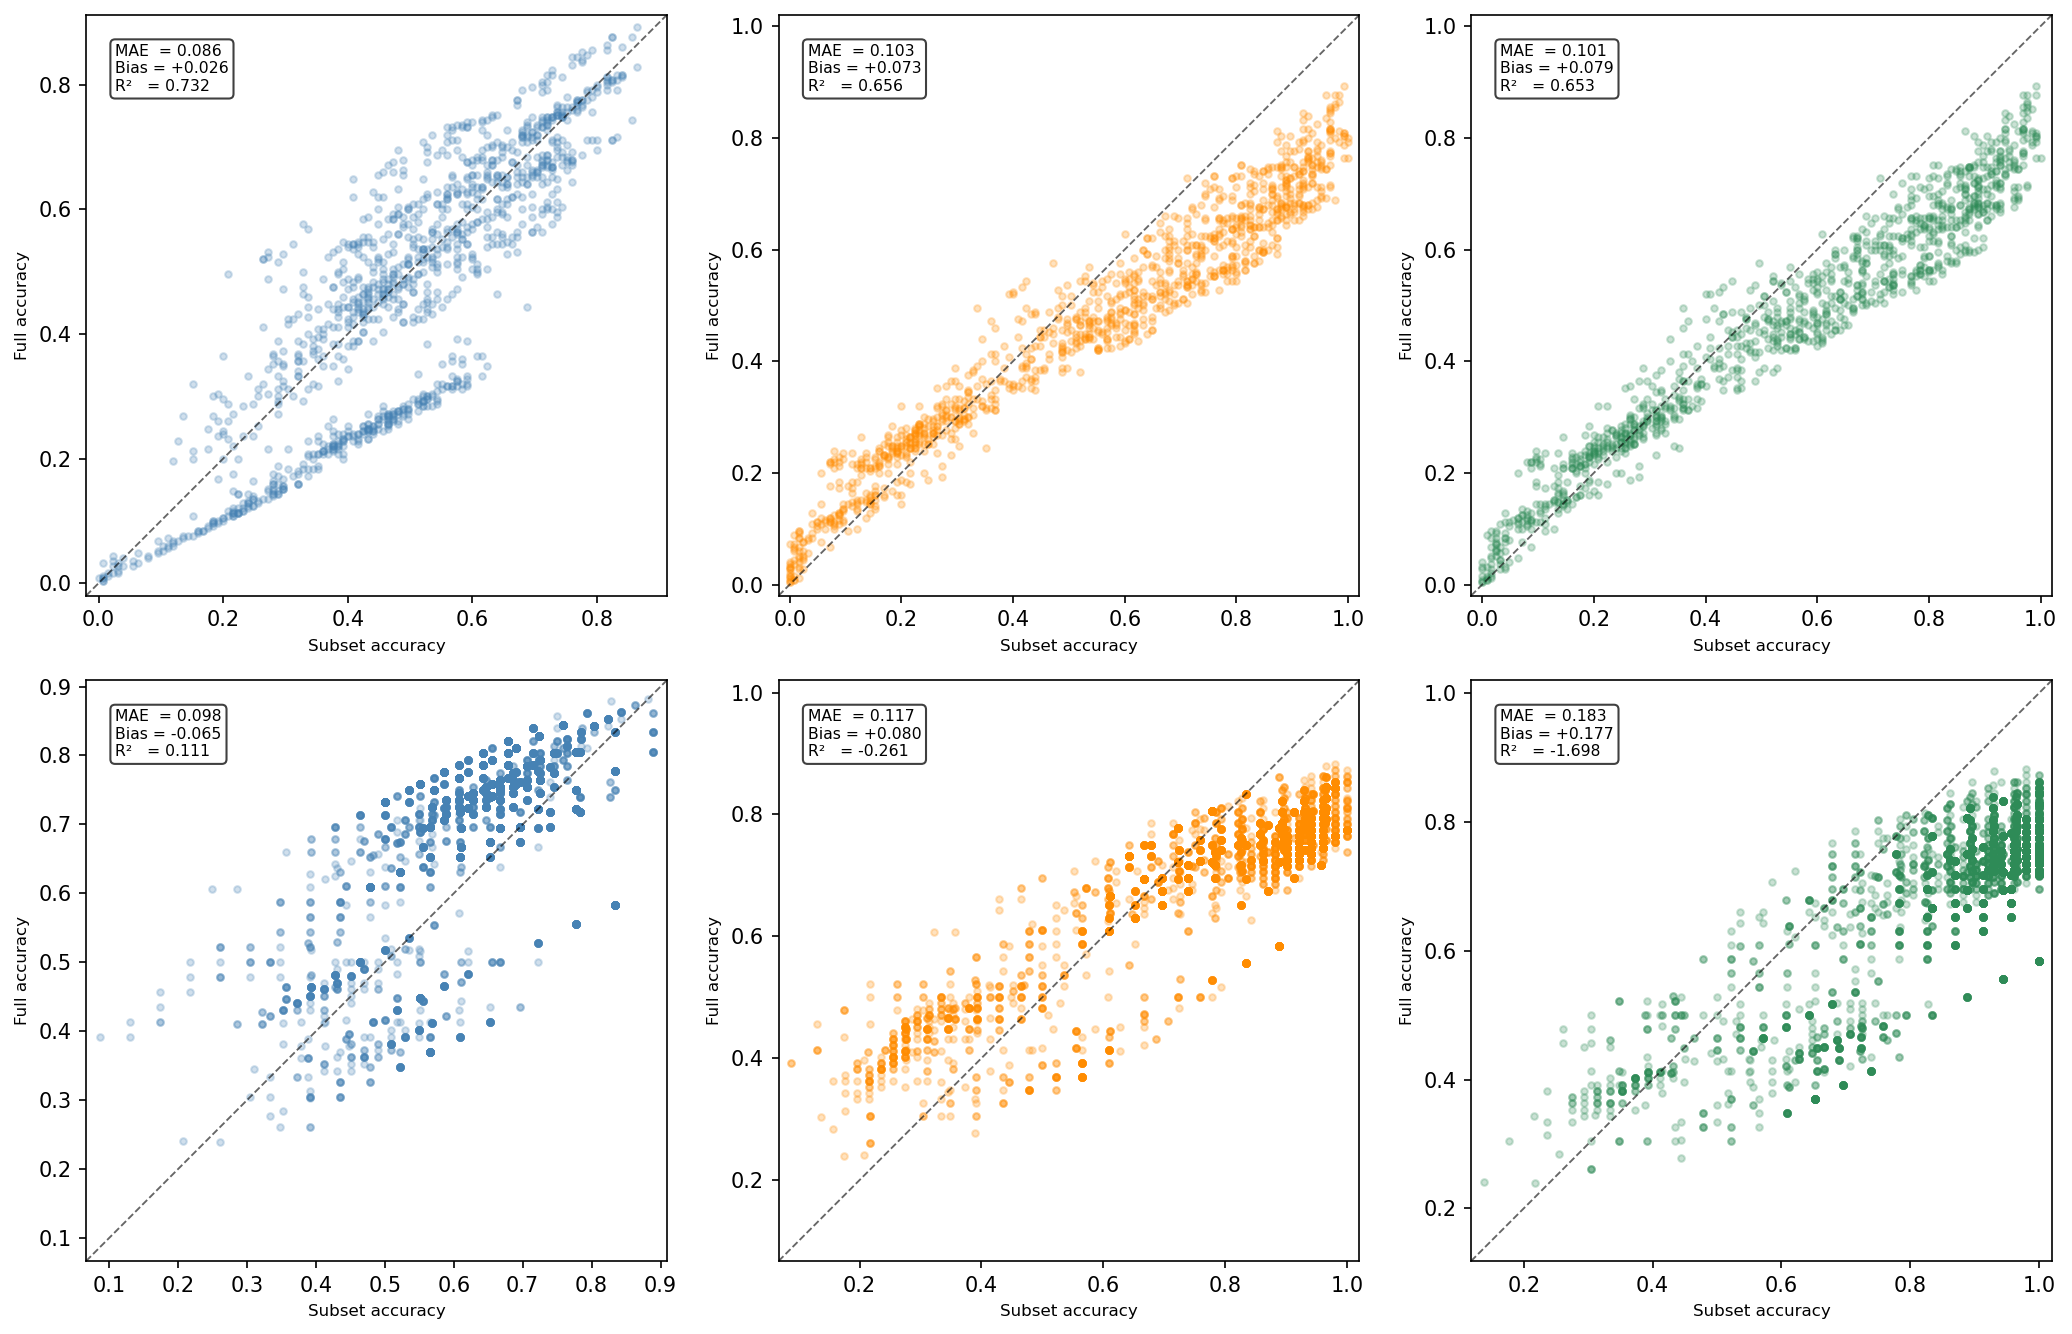
\includegraphics[width=\linewidth]{insample_accuracy_scatter}
  \caption{In-sample subset accuracy vs.\ full-benchmark accuracy for each
    (model, benchmark-slice) pair. Rows: MGSM (top) and MMLU (bottom).
    Columns: 1PL, 2PL, 3PL.
    Dashed line is $y = x$ (ideal); each panel is annotated with mean absolute error
    (MAE), Spearman $\rho$, and mean signed bias (subset $-$ full).
    1PL points track the diagonal tightly with low bias; 2PL and 3PL scatter widely
    and show systematic overestimation on MMLU.}
  \label{fig:insample_scatter}
\end{figure*}

\paragraph{Held-out accuracy prediction (Figure~\ref{fig:heldout_scatter}).}
The held-out evaluation re-fits IRT on 80\% of models and measures accuracy
prediction on the remaining 20\%.
For 1PL, the held-out MAE is nearly identical to in-sample on both benchmarks
(MGSM: $0.086$ held-out vs.\ $0.086$ in-sample; MMLU: $0.090$ vs.\ $0.098$),
and the directional bias is unchanged, confirming that 1PL item selection
generalizes to unseen models without any degradation in accuracy-prediction quality.
For MGSM 2PL, held-out MAE ($0.208$) is comparable to in-sample ($0.103$ in-sample is
for all models; held-out evaluates on the 20\% unseen split), reflecting that MAP
discrimination estimates generalize reasonably to unseen models within MGSM.
For MMLU, 2PL and 3PL retain moderate-to-large positive bias ($+0.183$ and $+0.168$
respectively) in held-out evaluation, confirming that the positive accuracy bias
is a structural property of discrimination-weighted item selection on knowledge-intensive
benchmarks rather than an in-sample artefact.

\begin{figure*}[t]
  \centering
  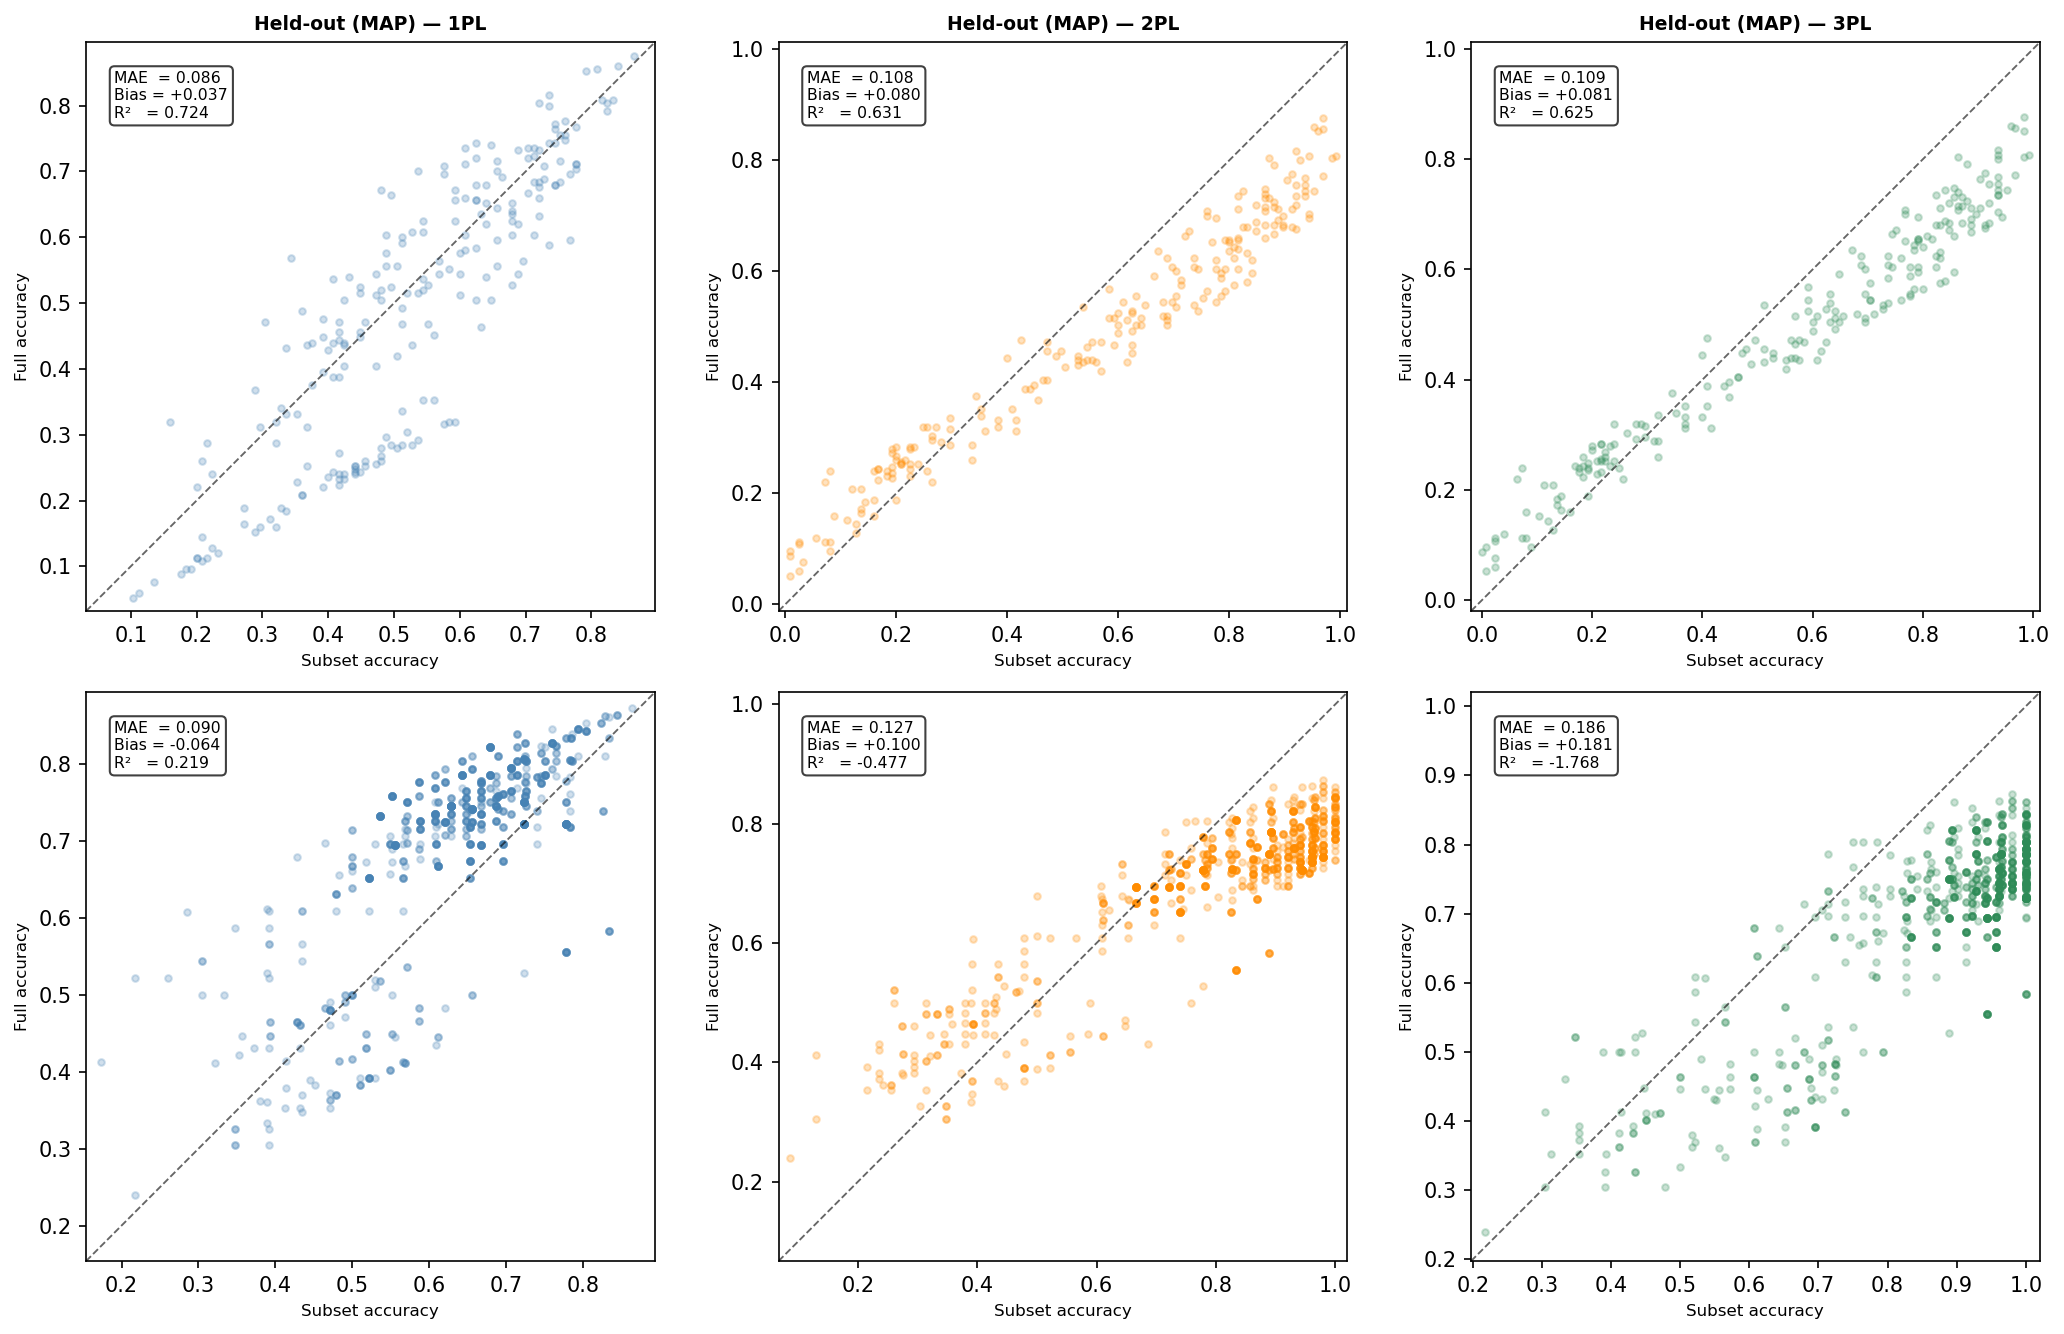
\includegraphics[width=\linewidth]{heldout_accuracy_scatter}
  \caption{Held-out subset accuracy vs.\ full-benchmark accuracy.
    IRT re-fitted on 80\% of models; each point is one (held-out model,
    benchmark-slice) pair ($n = 220$ for MGSM; $n = 876$ for MMLU).
    Layout and annotation as in Figure~\ref{fig:insample_scatter}.
    1PL MAE and bias are essentially unchanged from in-sample;
    2PL and 3PL retain their large positive bias on MMLU.}
  \label{fig:heldout_scatter}
\end{figure*}




\end{document}
